\documentclass[oneside]{ZJUthesis}
% 该文档中首字符为“%”的均为注释行,不会在论文中出现

% 论文默认为单面模式,需单面模式请将第一行换为如下所示:
% \documentclass[twoside]{ZJUthesis}

% 取消目录中链接的颜色,方便打印7778
% 如需颜色,请将“false”改为“true”
\hypersetup{colorlinks=true}

% 这里几行代码使得目录中的“第几章” 和后面的章节名称不致发生重叠
\makeatletter
\renewcommand{\numberline}[1]{%
\settowidth\@tempdimb{#1\hspace{0.5em}}%
\ifdim\@tempdima<\@tempdimb%
  \@tempdima=\@tempdimb%
\fi%
\hb@xt@\@tempdima{\@cftbsnum #1\@cftasnum\hfil}\@cftasnumb}
\makeatother


\begin{document}
%%%%%%%%%%%%%%%%%%%%%%%%%%%%%
%% 正文字体设定
%%%%%%%%%%%%%%%%%%%%%%%%%%%%%
\songti

%%%%%%%%%%%%%%%%%%%%%%%%%%%%%
%% 论文封面部分
%%%%%%%%%%%%%%%%%%%%%%%%%%%%%
% 中文封面内容

% 中图分类号
\classification{TM863}

% 单位代码
\serialnumber{10335}

% 密级,如需密级则将其前“%”去掉
%\SecretLevel{绝密}

% 学号
\PersonalID{11011010}

\title{基于成本的钉耙强度与应用}
% 如果标题一行写不下,就写成两行,在下面的命令里写第二行,不需要两行则注释掉
\titletl{——东方视角分析}

%英文题目
\Etitle{Cost Based Rake Strength}
% 如果一行写不下,同中文题目设定,一行写不下则写两行,不需要就注释掉
\Etitletl{and Application:}
\Etitletll{An Oriental View}

% 作者
\author{猪八戒}
\Eauthor{Bajie Zhu}

\degree{硕士}
\Edegree{Master of Engineering}

% 导师
\supervisor{唐三藏法师}
\Esupervisor{Master Sanzang Tang}

% 合作导师,如果有的话,去掉注释,
% \cpsupervisor{张三丰真人}
% \Ecpsupervisor{Truman Sanfeng Zhang}

% 专业名称
\major{祭坛管理}
\Emajor{Altar Management}

% 研究方向
\researchdm{法器工程}
\Eresearchdm{Ritual Instrument Engineering}

% 所属学院
\institute{大雷音寺管理研究院}
\Einstitute{Management Institute of Great Thunder Monastery}

%论文提交日期
\submitdate{二〇一三年一月十日}
\Esubmitdate{2013-1-10}

% 答辨日期
%\defenddate{2011年11月1日}

% 生成封面
\makeCoverPage

% 生成英文封面
\makeECoverPage

%%%%%%%%%%%%%%%%%%%%%%%%%%%%%%
%% 原创声明与版权协议页
%%%%%%%%%%%%%%%%%%%%%%%%%%%%%%

% 生成原创声明与版权协议页
\makeOSandCPRTpage


%%%%%%%%%%%%%%%%%%%%%%%%%%%%%%
%% 论文部分开始
%%%%%%%%%%%%%%%%%%%%%%%%%%%%%%
\ZJUfrontmatter

%%%%%%%%%%%%%%%%%%%%%%%%%%%%%%
%% 摘要
%%%%%%%%%%%%%%%%%%%%%%%%%%%%%%
\begin{abstract}
人工智能技术的更新正不断影响着人们的生活,近年来愈来愈多的用户采用人机对话的方式来高效地获取优质服务。
跨界服务平台是各类跨界服务集成的支撑系统,将跨越不同行业、组织、价值链等边界的服务进行深度融合和模式创新,
为用户提供多维度、高质量、富价值的跨界服务,成为现代服务业发展的重要创新途径,
相比传统的服务集成,跨界服务融合需开展模式、生态、环境、质量、价值等多维深度融合,
导致内部服务种类繁多、数量庞大,用户在进入系统后,面对如此量级的服务,用户在服务检索时需要花费大量时间,
同时也无法快速查询到与自己意图匹配的服务,因此如何提升用户检索服务时的体验成为问题。

借助人机对话的思想,本文在跨界服务平台中引入服务智能调用引擎。用户进入平台以后,可以输入带有意图的语句,如“查询成都开往杭州的火车票”,
服务智能调用引擎接受语句以后进行包含服务分类、接口分类和参数提取(语义槽填充)三项任务的语义理解,识别并找出系统内部与之匹配的服务,
从句子中提取服务调用必需的参数完成调用返回结果,从而解决了用户检索服务困难的问题。
服务智能调用引擎的核心是语义理解,语义理解模型的性能优劣是衡量调用引擎的智能化程度的重要标准,语义理解的结果也直接影响了服务检索和后续的服务调用。
当前,中文语义理解任务有着诸多困境,如特定下游任务缺乏充分的相关数据集,用户表述意图模糊、随意不规范,一词多义等,因此相关研究受到密切关注,
同时语义理解作为自然语言处理领域的基石性任务,它的研究具有重大科研意义和应用用途。

针对跨界服务领域中文语料匮乏的现状,本文在公开数据集基础上借助搜索引擎和课题组成员人工补充,构建了跨界服务领域的语义理解数据集。
扩充后的数据集包含8个服务类别,每条语料都包含对应的服务类别、接口类别和语义槽标注,共计19145条数据。
同时,本文提出了端到端的服务分类、接口分类和参数提取三项任务交互式联合识别模型,并引入bert作为预训练模型进行微调,
与三项任务独立处理的模型、基于word2vec的模型做了对照实验,验证了模型的可行性和优越性,其中表现最好的bert-co-interactive模型Sentence Acc达到91.47\%。
为将算法应用到实际,依托国家重点研发计划专项《现代服务业共性关键技术研发及应用示范》的子课题《跨界服务集成方法与支撑载体》的原型系统JTangYdrail,
设计了服务智能调用引擎的系统架构,让引擎能与现有平台相结合。

\keywords{跨界服务,文本分类,语义槽填充,意图识别,BERT}
\end{abstract}


%%%%%%%%%%%%%%%%%%%%%%%%%%%%%%
%% 英文摘要
%%%%%%%%%%%%%%%%%%%%%%%%%%%%%%
\begin{englishabstract}
The cross-border service network can break through the traditional organization, business and domain boundaries, 
and has become the main tool to promote cross-enterprise, cross-domain and cross-industry cooperation. 
However, the cross-border service network has a wide variety and huge number of internal services,
users have to spend a lot of cost in service retrieval when facing such a service. 
Therefore, how to improve the user's retrieval service experience becomes a problem. With the help of man-machine dialogue, 
this paper introduces an intelligent service invocation engine into the cross-border service network system. 
The engine can identify? the matching service within the system according to the sentence passed in by the user
and extract the necessary parameters for the service call from the sentence to complete the call and return the result. 
The core of the engine is semantic understanding model. Its performance is an important criterion to measure the degree of engine intelligence, 
and it also directly affects subsequent service calls. At present, Chinese semantic understanding tasks have many challenges, 
such as lack of sufficient data sets for specific downstream tasks, vague user expression intentions, polysemous words, etc. 
At the same time, semantic understanding is the cornerstone of natural language processing, so its research has great significance and application prospects. 

In view of the lack of Chinese corpus in the field of cross-border services, 
this paper builds a semantic understanding data set in the field of cross-border services based on the public data set with the help of search engines and artificial supplements by members of the research team. 
The expanded data set contains 8 service categories, and each corpus contains corresponding service category, 
interface category and semantic slot annotations. At the same time, 
this paper proposes an end-to-end interactive joint recognition model, 
introducing bert as a pre-training model and a knowledge base to enhance the semantics of short text input.
we do control experiments with other models to verify the feasibility and superiority of the model,
Among them, the best-performing bert-co-interactive model's Sentence Acc reached 91.47\%. 
In order to apply the algorithm to practice, 
relying on the prototype system JTangYdrail of the sub-project "Cross-border Service Integration Methods and Support Carriers" of the National Key Research and Development Program "Modern Service Industry Common Key Technology Research and Development and Application Demonstration", 
The system architecture of service intelligent call engine was designed,which allows the engine to be integrated with the existing platform.

\englishkeywords{Natural Language Understanding,Text Classification, Slot Filling, Intent Detection,BERT}
\end{englishabstract}


%%%%%%%%%%%%%%%%%%%%%%%%%%%%%%
%% 目录页
%%%%%%%%%%%%%%%%%%%%%%%%%%%%%%
\ZJUcontents

%%%%%%%%%%%%%%%%%%%%%%%%%%%%%%
%% 插图列表
%%%%%%%%%%%%%%%%%%%%%%%%%%%%%%
\ZJUListofFigures

%%%%%%%%%%%%%%%%%%%%%%%%%%%%%%
%% 表格列表
%%%%%%%%%%%%%%%%%%%%%%%%%%%%%%
\ZJUListofTables


%%%%%%%%%%%%%%%%%%%%%%%%%%%%%%
%% 正文内容部分开始
%%%%%%%%%%%%%%%%%%%%%%%%%%%%%%
\ZJUmainmatter

 \chapter{绪论}

\section{课题背景与研究意义}

依托以互联网为代表的信息技术的高速发展,我国社会当前正处在由传统服务业向现
代服务业全面升级的重要历史进程中。充分利用和结合现代先进的信息技术,提供信息和
知识更加密集、附加值更高的服务是现代服务业的基本要求。互联网作为现代信息服务的
载体,从早期简单的门户网站、搜索引擎,发展到社交网站、即时通信,再到移动搜索、LBS
等移动互联网应用的风靡,在产业规模持续扩大的同时,也不断向各行各业渗透,从早期
的传媒、游戏等行业,到娱乐、零售行业,再到金融、教育和医疗等行业,影响范围还在不
断继续扩大\cite{王晓玲2015我国现代服务业借力}。由此可见,未来服务的基础形态一定是基于互联网的,各行业通过互联网来
提供他们的服务是大势所趋。

跨界服务将跨越不同行业、组织、价值链等边界的服务进行深度融合和模式创新,为用户提供多维度、高质量、富价值的跨界服务,成为现代服务业发
展的重要创新途径。跨界服务平台是各类跨界服务集成的支撑系统,相比传统的服务集成,跨界服务融合需开展模式、生态、环境、质量、价值等多维深度融合,
导致内部服务种类繁多、数量庞大,用户在进入系统后,面对如此数量的服务,很难快速检索到想要的服务,面向用户的服务检索以及如何提升用户体验成为问题。

随着人工智能的飞速发展,人机对话越来越受到人们的关注。人机对话系统主要由自动文本\&语音识别,语义理解,对话内容管理,
对话内容生成和交互组成。在人机对话过程中,面向任务的对话最紧急的事情要做的是获取用户的真实意图。经过一轮或多轮对话后的上下文综合判断,
可以准确捕捉用户的意图并尽快完成面向任务的对话。
这其中最重要的一环是语义理解,直接影响到系统能否提取用户需求,语义理解可被分为领域分类、意图识别和语义槽填充三个子模块。
意图检测作为自然语言理解的一个子模块,在提高自然语言理解和口语理解方面起着至关重要的作用。
领域、意图检测设法捕获用户的真实意图和用户的期望动作,例如饭店预订,机票查询等。语义槽填充可视为序列标注,主要工作是实体提取,需要在语义层面更细粒度的理解。

借助人机对话的思想,本文在跨界服务平台中引入服务智能调用引擎。用户进入平台以后,可以输入带有自己意图的语句,如“查询成都开往杭州的火车票”,
服务智能调用引擎接受语句以后进行语义理解,识别并找出系统内部与之匹配的服务,从句子中提取参数完成调用返回结果,从而解决了用户检索服务困难的问题,
简化了用户操作,提升了用户体验,让系统更加智能化。


\begin{figure}[htbp]
  \centering
  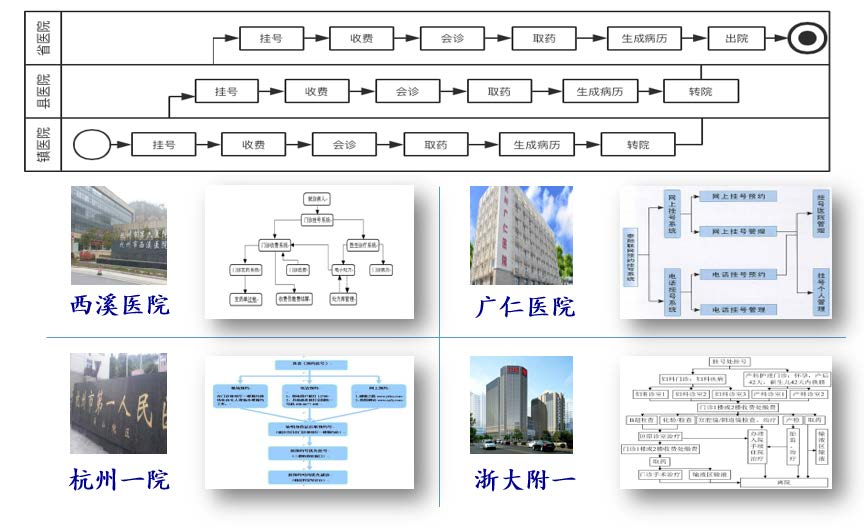
\includegraphics[scale=1]{./images/hospitalRunningModel.jpg}
  \caption{跨界服务}
  \label{fig:kuajiefuwu}
\end{figure}


现代服务业是中国经济发展战略中的重要组成部分,也是衡量一个国家经济发展水平
的重要标志。推动现代服务业的发展壮大已成为当前中国经济发展的重要目标和关键动力。
服务计算作为现代服务业发展的重要技术基础,需要结合现代服务业发展的具体场景和具体问题进行深入的研究和应用。
本文依托于国家重点研发计划专项《现代服务业共性关键
技术研发及应用示范》的子课题《跨界服务集成方法与支撑载体》,围绕在研究跨界服务集
成和交互过程中发现的服务种类数量繁多用户检索困难、交互缺乏智能化的问题,在跨界服务平台中引入服务智能调用引擎,解决了用户检索服务困难的问题,
简化了用户操作,提升了用户体验,让系统更加智能化。

同时,本文着重研究了智能调用中的语义理解,语义理解是自然语言处理任务的重要基石,作用是使计算机能够对人类语言的结构和含义的理解,
从而允许用户使用自然句子与计算机进行交互。本文提出文本分类和语义槽填充模型,不局限于跨界服务场景,对模型稍作修改,可应用于许多
其他的同类型任务中,如情感分析,内容分析,任务型对话系统等。本文将NLU技术应用于跨界服务领域,拓宽了自然语言处理技术的界限。

综上所述,本文在跨界服务平台基于深度学习算法设计并实现了服务智能调用引擎,跨界服务系统利用深度学习模型提取分析用户输入的语句的语义,
在系统内部检索匹配服务自动执行返回结果展示,完成服务的智能化调用。

\section{国内外研究现状}
\subsection{跨界服务}
“云大物移智”等新一代信息技术的发展与应用,使得人类的认知扩大、能力增强,
也将重新定义传统边界。“跨界”即突破原有界限,实现界内和界外资源的整合与协作。
跨界服务将跨越不同行业、组织、价值链等边界的服务进行深度融合和模式创新,为用
户提供多维度、高质量、富价值服务,这不仅是技术发展的必然,也是现代服务业发展
的重要创新途径。

相比传统的服务集成,跨界服务融合需开展模式、生态、环境、质量、价值等多维
深度融合,具有极大挑战。目前国内外依然缺少跨界服务本质规模与模式认知、设计与
管理方法、质量管理与价值工程等方面的系统研究,也缺少相关工程方法和支撑载体。
从以下四个方面综述国内外的相关研究:

(1) 服务模式创新是推动现代服务业快速发展的重要因素。近年来,国际上出现
了以Artifact 为中心的商业流程建模方法、基于商业交易过程的商业模式分析框架等,
对服务模式进行了分析和建模;国内浙江大学首次提出了跨界服务概念及其3C 特点。
但总体来看,目前学术界在跨界服务本质规律认知、模式定量分析与评估等方面仍处于
探索阶段。

(2) 跨界服务设计关注如何获取和分析角色多元的用户真实需求,并根据用户需
求进行服务架构、流程和接口等生态设计。IBM 研究院、北京大学、武汉大学等单位的
研究团队在服务需求建模、服务设计和服务互操作性管理等方面具有较好的研究积累,
做出了一系列代表性工作如SOMA-ME、RGPS 需求元建模框架、基于Tropos 的服务建模
方法等,但针对跨界服务融合的设计目前仍缺少完整、系统的支撑方法体系。

(3) 跨界服务融合需要高效、可靠的运行支撑环境,以提供服务网络的运行态支
持。目前这一领域主要有企业服务总线、企业应用集成等相关技术,北京大学、IBM、
佐治亚理工学院等在云端融合资源服务化、服务总线等方面具有较好研究积累,但这些
技术大多针对企业级运行环境,仅实现服务的结构和信息融合,难以应对跨界服务所需
的多维深度融合、动态服务网络优化、开放环境安全管控等挑战。

(4)对服务系统进行精准的能力配置以提供特定的质量与价值,并在运行时准确
感知它们的实际提供水平以做出调控和改进。IBM 研究院、荷兰阿姆斯特丹自由大学、
哈尔滨工业大学等单位的研究团队在服务质量设计与度量、服务价值建模、服务价值感
知等方面具有较好的研究积累,做出了一系列代表性工作,如VASEM、服务价值网等,
但针对跨界服务质量体系和价值工程的研究仍处于初期阶段。

\subsection{文本分类}
文本分类任务使语义理解的重要组成部分,
文本分类是为给定的自然语言文本段自动分配零个,一组或多组预定义标签,选择标签以反映文本的“含义”。
文本分类应用在许多NLP任务中,例如情感分析,主题分类,问答系统和对话行为分类等。
图\ref{fig:textClassification}示出了文本分类中所涉及的主要技术,
文本数据不同于数字,图像或信号数据。它要求对NLP技术进行仔细处理。重要的第一步是预处理模型的文本数据。浅层学习模型通常需要通过人工方法获得良好的样本特征,然后使用经典的机器学习算法对其进行分类。因此,该方法的有效性在很大程度上受到特征提取的限制。但是,与浅层模型不同,深度学习通过学习一组非线性变换将特征工程直接映射到输出,从而将特征工程集成到模型拟合过程中。主要文本分类方法的示意图如图2所示。从1960年代到2010年代,基于浅层学习的文本分类模型占主导地位。浅层学习意味着基于统计的模型,例如朴素贝叶斯(NB)[10],K近邻(KNN)[11]和支持向量机(SVM)[12]。与早期的基于规则的方法相比,该方法在准确性和稳定性方面具有明显的优势。但是,这些方法仍然需要进行功能设计,这既耗时又昂贵。此外,它们通常会忽略文本数据中的自然顺序结构或上下文信息,这使学习单词的语义信息变得困难。自2010年代以来,文本分类已逐渐从浅层学习模型变为深层学习模型。与基于浅层学习的方法相比,深度学习方法避免了人工设计规则和功能,并自动为文本挖掘提供了语义上有意义的表示形式。因此,大多数文本分类研究工作都基于DNN,DNN是数据驱动的方法,具有很高的计算复杂性。很少有文章关注浅层学习模型来解决计算和数据的局限性。
\begin{figure}[htbp]
  \centering
  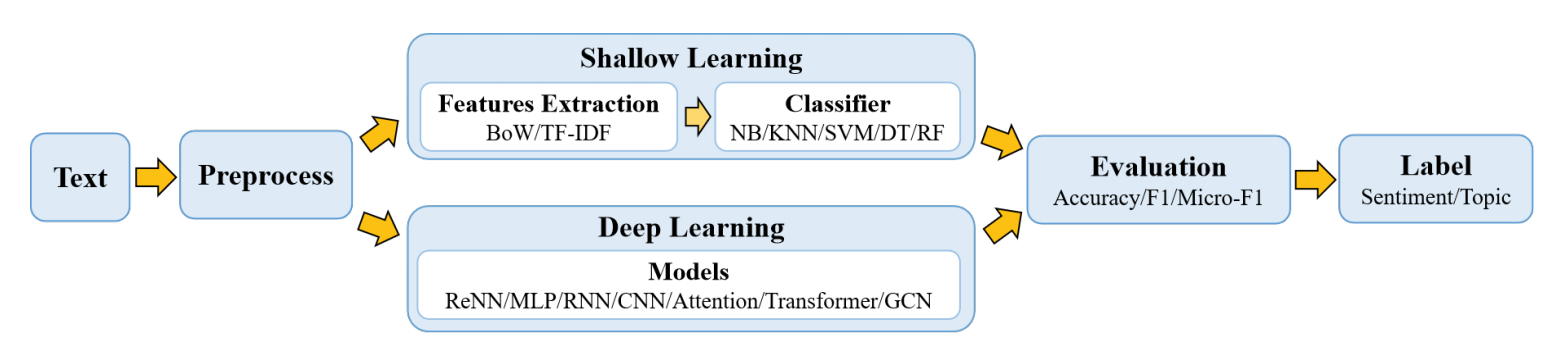
\includegraphics[scale=1]{./images/textClassification.png}
  \caption{文本分类技术研究发展趋势\cite{li2020survey}}
  \label{fig:textClassification}
\end{figure}


\subsection{命名实体识别}
语义槽填充任务可以视为命名实体识别(NER),NER的任务是识别文本范围内提及的命名实体,并将其分类为预定义的类别,
例如人名、位置、组织等。
尽管早期基于统计规则的NER系统产生了不错的识别精度,但是需要精心设计规则和特征,因此通常需要大量的人工。
近年来,深度学习已被应用于NER系统中,并产生了优异的性能。

NER的演变过程,如图\ref{fig:nerp}所示。MUC-6首次使用“命名实体”(NE),
其任务是识别文本中的组织名称,人名和地理位置以及货币,时间和百分比表达式。
关于NER中应用的技术,主流方法有以下几种:

\begin{figure}[htbp]
  \centering
  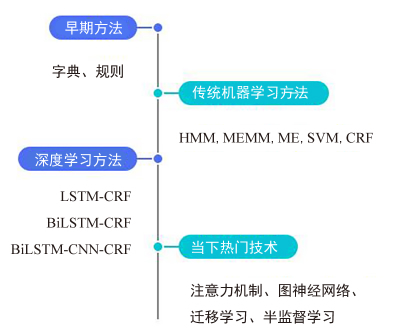
\includegraphics[scale=1]{./images/nerp.jpg}
  \caption{命名实体识别技术研究发展趋势\cite{nadeau2007survey}}
  \label{fig:nerp}
\end{figure}

(1)基于统计规则的方法

基于规则的NER系统依赖于人工手动制定的规则,可以基于特定领域的地名词典和句法词法模式设计规则。
Kim等提出使用布里尔规则推理方法进行语音输入,该系统会根据Brill的语音标记器自动生成规则\cite{kim2000rule},
% 在生物医学领域,Hanisch等提出了ProMiner,它利用预处理的同义词词典来识别生物医学文本中提及的蛋白质和潜在基因\cite{hanisch2005prominer}。 
Quimbaya等出了一种基于字典的电子健康记录中NER的方法\cite{pomares2016named},实验结果表明,该方法在对精度的影响有限的前提下可提高召回率。
其他一些基于规则的知名NER系统包括LaSIE-II,NetOwl,Facile,SAR,FASTUS和LTG,
这些系统主要基于手工制定的语义和语法规则来识别实体,当词汇详尽无穷时,基于规则的系统可以很好地工作。
但是,由于特定领域的定制规则和不完整的词典,此类系统中经常会出现高准确率和低召回率的现象,并且这些系统无法很好到迁移到其他域。

(2)无监督学习方法

无监督学习的一种典型方法是聚类,基于聚类的NER系统根据上下文相似性从聚类类簇中提取命名实体,
其核心思想是,可以使用在大型语料库上计算出的词汇资源,词汇模式和统计信息来推断命名实体。 
Collins等观察到,使用未标记的数据将对监督的要求减少到仅需7个简单的“种子”规则\cite{collins1999unsupervised},
然后,作者提出了两种用于命名实体分类的无监督算法。类似地,Etzioni等利用一组谓词名称作为输入,并利用一小组通用提取模式实现其识别过程\cite{etzioni2005unsupervised}。 
Nadeau等提出了一个非监督系统的地名词典建设和命名实体歧义解决方案,该系统基于简单而高效的启发式方法,结合了实体提取和歧义消除功能\cite{nadeau2006unsupervised}。
另外,Zhang和Elhadad提出了一种从生物医学文本中提取命名实体的无监督方法\cite{zhang2013unsupervised},
他们的模型求助于术语、语料库统计信息(例如逆文档频率和上下文向量)和浅层语法知识(例如名词短语分块),
在两个主流生物医学数据集上进行的实验证明了其无监督方法的有效性和可推广性。

(3)基于特征的监督学习方法

通过监督学习,NER被转换为多类别分类或序列标记任务。给定带标注的数据样本,特征经过精心设计以能够代表每个训练示例。
然后,利用机器学习算法来学习模型,从未标注数据中识别出相似的模式,特征工程在有监督的NER系统中至关重要。
许多机器学习算法成功应用于有监督的NER,包括隐马尔可夫模型(HMM),决策树,最大熵模型,支持向量机(SVM)
和条件随机场(CRF)。 Bikel等提出了第一个基于HMM的NER系统,名为IdentiFinder,用于识别分类名称,
日期,时间表达式和数字\cite{bikel1998nymble,bikel1999algorithm}。此外,Szarvas等通过使用决策树和AdaBoostM1学习算法开发了一种多语言NER系统,
它可以训练几个独立的决策树分类器,然后通过表决方案组合进行决策\cite{szarvas2006multilingual}。 
Borthwick等通过应用最大熵理论提出了“最大熵命名实体”(MENE),MENE能够在做出标记决策时利用各种知识资源。
 McNamee和Mayfield使用了1000种与语言相关的特征和258种拼字法和标点特征来训练SVM分类器,每个分类器都会做出决策,即当前token是否属于八个类别之一\cite{mcnamee2002entity}。
 在预测实体标签时,SVM没有考虑相邻词之间的联系,CRF则考虑了上下文。 
 McCallum和Li提出了NER中CRF的特征归纳方法,在CoNLL03上进行了实验,成绩达到了84.04%\cite{mccallum2003early}。 
 Krishnan和Manning提出了一种基于两个耦合CRF分类器的两阶段方法,第二个CRF利用从第一个CRF的输出中得到的潜在表示\cite{krishnan2006effective}。

 (4)深度学习方法

 近年来,基于DL的NER模型逐渐占据主导地位,并取得了最优异的成果,与基于特征的方法相比,深度学习能够自动发现隐藏的特征。 
 将深度学习技术应用于NER有三个核心优势,首先,NER受益于非线性变换,该变换生成从输入到输出的非线性映射。
 与线性模型(对数线性HMM和线性链CRF)相比,基于DL的模型能够通过非线性激活函数从数据中学习复杂的特征。
 其次,深度学习为设计NER特诊节省了大量精力,传统的基于特征的方法需要大量的人力和领域专业知识,
 基于DL的模型可有效地从原始数据中自动学习有用的表示形式和潜在特征。
 第三,可以通过梯度下降在端到端模型中训练深度神经NER模型,此特性使我们能够设计复杂的NER系统。
 BiLSTM-CRF是使用深度学习的NER最常见的体系结构,
 以cloze-style方式预训练双向Transformer模型的方法在CoNLL03上实现了最优异的性能(93.5%)\cite{baevski2019cloze}。 
 Zhang 和 Yang 提出了一种针对中文NER的格子结构LSTM模型,该模型对输入字符序列以及与词典匹配的所有潜在单词进行编码\cite{zhang2018chinese}。
 除中文外,许多研究使用其他语言进行
 每种语言都有其自己的特征,有许多研究旨在通过将知识从源语言迁移到标签很少或数据量很少的目标语言来解决NER中的跨语言问题。
%  输入的分布式表示形式考虑了单词和字符级别的嵌入,现有的分类法基于字符级编码器,单词级编码器和标签解码器,以及结合了对功能有效的POS标签和地名词典等附加功能,
%  上下文编码器将使用CNN,RNN或其他网络捕获上下文相关性,标签解码器为输入序列中的token预测标签。
%  例如,在图\ref{fig:nerDL}中,每个token都被预测为带有其类型的命名实体:即带有B-(开头),I-(内部),E-(结束),S-(单个),或O-(外部)的命名实体。
%  当然,还有其他标记方案或标记符号,例如BIO。还可以训练标签解码器以检测实体边界,然后将检测到的文本跨度分类为实体类型。


% NER系统的成功很大程度上取决于其输入的表示形式,集成或微调预训练的语言模型嵌入正成为神经NER的研究热点,
% 利用这些语言模型嵌入时,可以显着提高性能。
% 我们从三个角度讨论利弊:输入,编码器和解码器。 
% 首先,关于是否应该使用外部知识或如何将其集成到基于DL的NER模型尚未达成共识,
% 一些研究表明,外部知识可以提高NER的表现。
% 但是,缺点也很明显:1)获得外部知识是劳动密集型的(例如地名词典)或计算上昂贵的(例如依赖项); 2)整合外部知识会对端到端学习产生不利影响,并损害基于DL的系统的通用性。
% 其次,当在大型语料库上对Transformer进行预训练时,Transformer编码器比LSTM更有效。如果未预先训练且训练数据有限,则Transformer将无法完成NER任务\cite{guo2019star,yan2019tener}。
% 第三,RNN和Pointer Network解码器的主要缺点在于贪婪解码,这意味着当前步骤的输入需要上一步的输出。此机制可能会对速度产生重大影响,并且是并行化的障碍。 
% CRF是标签解码器的最常见选择,当采用非语言模型(即非上下文化)嵌入(例如Word2vec和GloVe)时,CRF可以具有强大地捕获标签转换相关性的能力。
% 但是,当实体类型的数量很大时,CRF在计算上可能会很缓慢。更重要的是,当采用上下文化语言模型嵌入(例如BERT和ELMo )时,与softmax分类相比,CRF并不总是导致更好的性能。
% 对于最终用户,选择哪种体系结构取决于数据和域任务。如果数据丰富,则可以考虑从头开始使用RNN训练模型,并对上下文语言模型进行微调。
% 如果数据稀缺,则采用迁移的策略可能是更好的选择。对于新闻专线领域,有许多可用的预训练的现成模型。对于特定领域(例如,医学和社交媒体),
% 使用特定领域的数据对通用的上下文化语言模型进行微调通常是一种有效的方法。NER适用于不同的语言,主要关注英语和一般领域的NER。
% 除了英语以外,还有许多其他语言或跨语言环境的研究。


迁移学习旨在通过利用从源域中学到的知识来在目标域上执行机器学习任务\cite{pan2009survey},在NLP中迁移学习也称为领域适应,
在迁移学习的设置中,不同的神经模型通常在源任务和目标任务之间共享模型参数的一部分。。 
Pan等提出了跨域ner的转移联合嵌入(TJE)方法,TJE使用标签嵌入技术将多类别分类转换为低维空间中的回归问题\cite{pan2013transfer}。 
Qu等观察到相关的命名实体类型通常共享词汇和上下文特征\cite{qu2016named},他们的方法使用两层神经网络来学习源命名实体类型和目标命名实体类型之间的相关性,
适用于源域与目标域具有相似(但不相同)的NER问题。 
Peng和Dredze在多任务学习环境中探索了迁移学习\cite{peng2016multi},他们在新闻和社交媒体这两个领域中分别考虑了:分词和NER这两项任务。
Yang等首先研究了神经网络的不同层的可迁移性\cite{yang2017transfer},然后,他们针对跨域、跨语言和跨应用程序场景提出了三种不同的参数共享架构:
如果两个任务具有可映射的标签集,则存在一个共享的CRF层,否则,每个任务将学习一个单独的CRF层。
实验结果表明,在资源匮乏的情况下(即更少的可用标签),各数据集的跑分成绩都有了显著改善。 
赵等提出了一种具有领域适应性的多任务模型,其中全连接层适用于不同的数据集,但CRF特征是分别计算的,其主要优点是,
在数据选择过程中会过滤掉分布不同且标注未对齐的实例\cite{zhao2018improve}。



\section{主要工作与组织结构}
本文在跨界服务平台中引入服务智能调用引擎,主要研究了系统对用户输入语句的语义理解,主要解决了NLU中的领域分类(在本文中称为服务分类)、意图识别(在本文中称为接口分类)
和语义槽填充(在本文中称为参数提取),
分别使用了传统深度学习方法和结合预训练模型的联合识别方法对算法性能不断优化。同时为将算法落地应用到系统中,在跨界服务平台系统中设计和开发了服务智能调用引擎模块。本文
的主要研究工作如下:

(1)本文调研了现有语义理解算法以及主要用途,分析了语义理解背后涵盖的子问题,并将提出的语义理解算法应用在跨界服务领域,拓宽了算法的应用界限。

(2)为解决跨界服务平台中服务智能调用的问题,离不开充分的数据。在调研语义理解相关的公开数据集后,发现高质量的可用于跨界服务平台的中文语料数据集相对匮乏,
为此,本文在已有数据集SMP2019ECDT上,筛选了跨界服务平台中用户使用较多的几类服务的语料信息做补充和扩展,构建了跨界服务相关的中文预料数据集,共19145条数据组成实验
数据集,同时可用于后续的相关研究。

(3)对于语义理解任务,对传统深度学习方法做了局部优化,在此基础上,提出结合预训练模型的交互式联合识别模型对算法进行优化,在本文构建的数据集训练完成后,测试集的评分表现
均高于传统方法,领域分类(在本文中称为服务分类)准确率为95.18\%,意图识别(在本文中称为接口分类)准确率为94.91\%,语义槽填充(在本文中称为参数提取)$F_1$值为92.23\%,
句子整体准确率为91.47\%。同时利用消融分析等方法,设置了多组对照实验,验证模型的优越性。

(4)为将算法落地应用到系统中,在跨界服务平台系统中设计和开发了服务智能调用引擎模块,在实际应用了算法的可行性。

本文基于跨界服务系统中服务智能调用的课题背景,只要展开对服务分类、接口分类和参数填充算法的研究,行文共分七章,各章主要内容如下:

第一章:绪论。介绍了跨界服务系统中服务智能调用的研究背景与意义

% \chapter{相关技术与理论基础}

\section{词向量表示}

词嵌入(word embedding)能够捕获文本中词语的上下文,语义,句法相似性,是词汇最流行的表示形式之一。
Word2Vec使用浅层神经网络学习单词嵌入,由Tomas Mikolov于2013年在Google上提出\cite{mikolov2013distributed},
它的输入来源是一个大的单词语料库。
Word2Vec是具有单个隐藏层的简单神经网络,并且像所有神经网络一样具有权重,在训练过程中其目标是调整这些权重以使损失函数更小\cite{goldberg2014word2vec}。 
但是,Word2Vec训练时并没有处理任何任务,或者说进行的任务本身没有意义,训练完成后仅使用其隐藏层的权重,将其用作词嵌入,然后将模型的其余部分剔除。
类似的思想在无监督的特征表达中也有用到,即训练了自编码器以在隐藏层中压缩输入向量,然后将其解压缩回输出层中,解压缩的标签任为原始向量,
训练完成后剥离输出层仅使用隐藏层,因为它通过学习具有了良好的编码能力。
如果不同的单词语义相似,那么当这些单词作为输入传递进网络时,Word2Vec应该具有相似的输出,
这些单词在隐藏层中计算出的单词矢量必须相似。
Word2Vec能够捕获单词之间的多个不同维度的相似度,从而可以使用词向量来表示语义和句法模式。
可以通过对这些单词的词向量进行代数运算来生成诸如“男人之于女人等于兄弟之于姐妹”的模式,
从而使“兄弟”-“男人” +“女人”的词向量与“姐妹”的词向量表示十分接近。

Word2Vec是一种从原始文本中学习单词嵌入计算效率特别高的预测模型,
它主要有连续词袋(CBOW)模型和Skip-Gram模型两种方式。
CBOW模型:此方法将每个单词的上下文作为输入,并尝试预测与上下文相对应的单词。
如图\ref{fig:CBOW}所示,CBOW模型取用C个上下文词,输入是他们的onehot表示,乘以共享矩阵W(维度是V×N)求均值
得到的结果作为隐藏层,一个N维的长条状矩阵,隐藏层向量乘以输出权重矩阵得到输出向量,即为从上下文
中处在当前位置的单词的向量表示。训练完成后仅使用其隐藏层的权重,将其用作词嵌入,然后将模型的其余部分剔除。
Skip-Gram模型:给定一个处在句子中单词,Skip-gram模型的训练任务是尝试预测其相邻单词,和CBOW做的处理正好相反。
可以看到,在cbow方法中,是用上下文词预测当前词,训练过程中使用梯度下降方法,不断的调整相邻上下文词的向量。
而skip-gram模型是用观察到的词来预测上下文词,训练过程中使用梯度下降法不断的调整当前词的词向量。

\begin{figure}[htbp]
  \centering
  % \hspace{-7mm}
  \subfloat[CBOW]{
  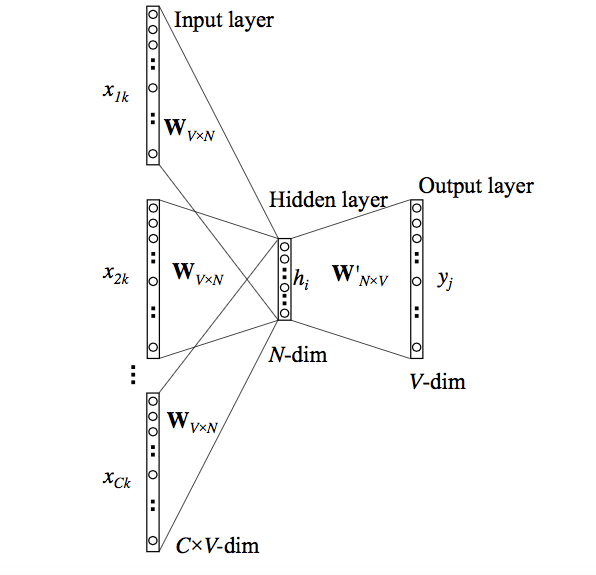
\includegraphics[width=6cm]{./images/CBOW.jpg}
  \label{fig:CBOW}
  }
  % \hspace{5pt}
    % \hspace{+5mm}
  \subfloat[skip-gram]{
  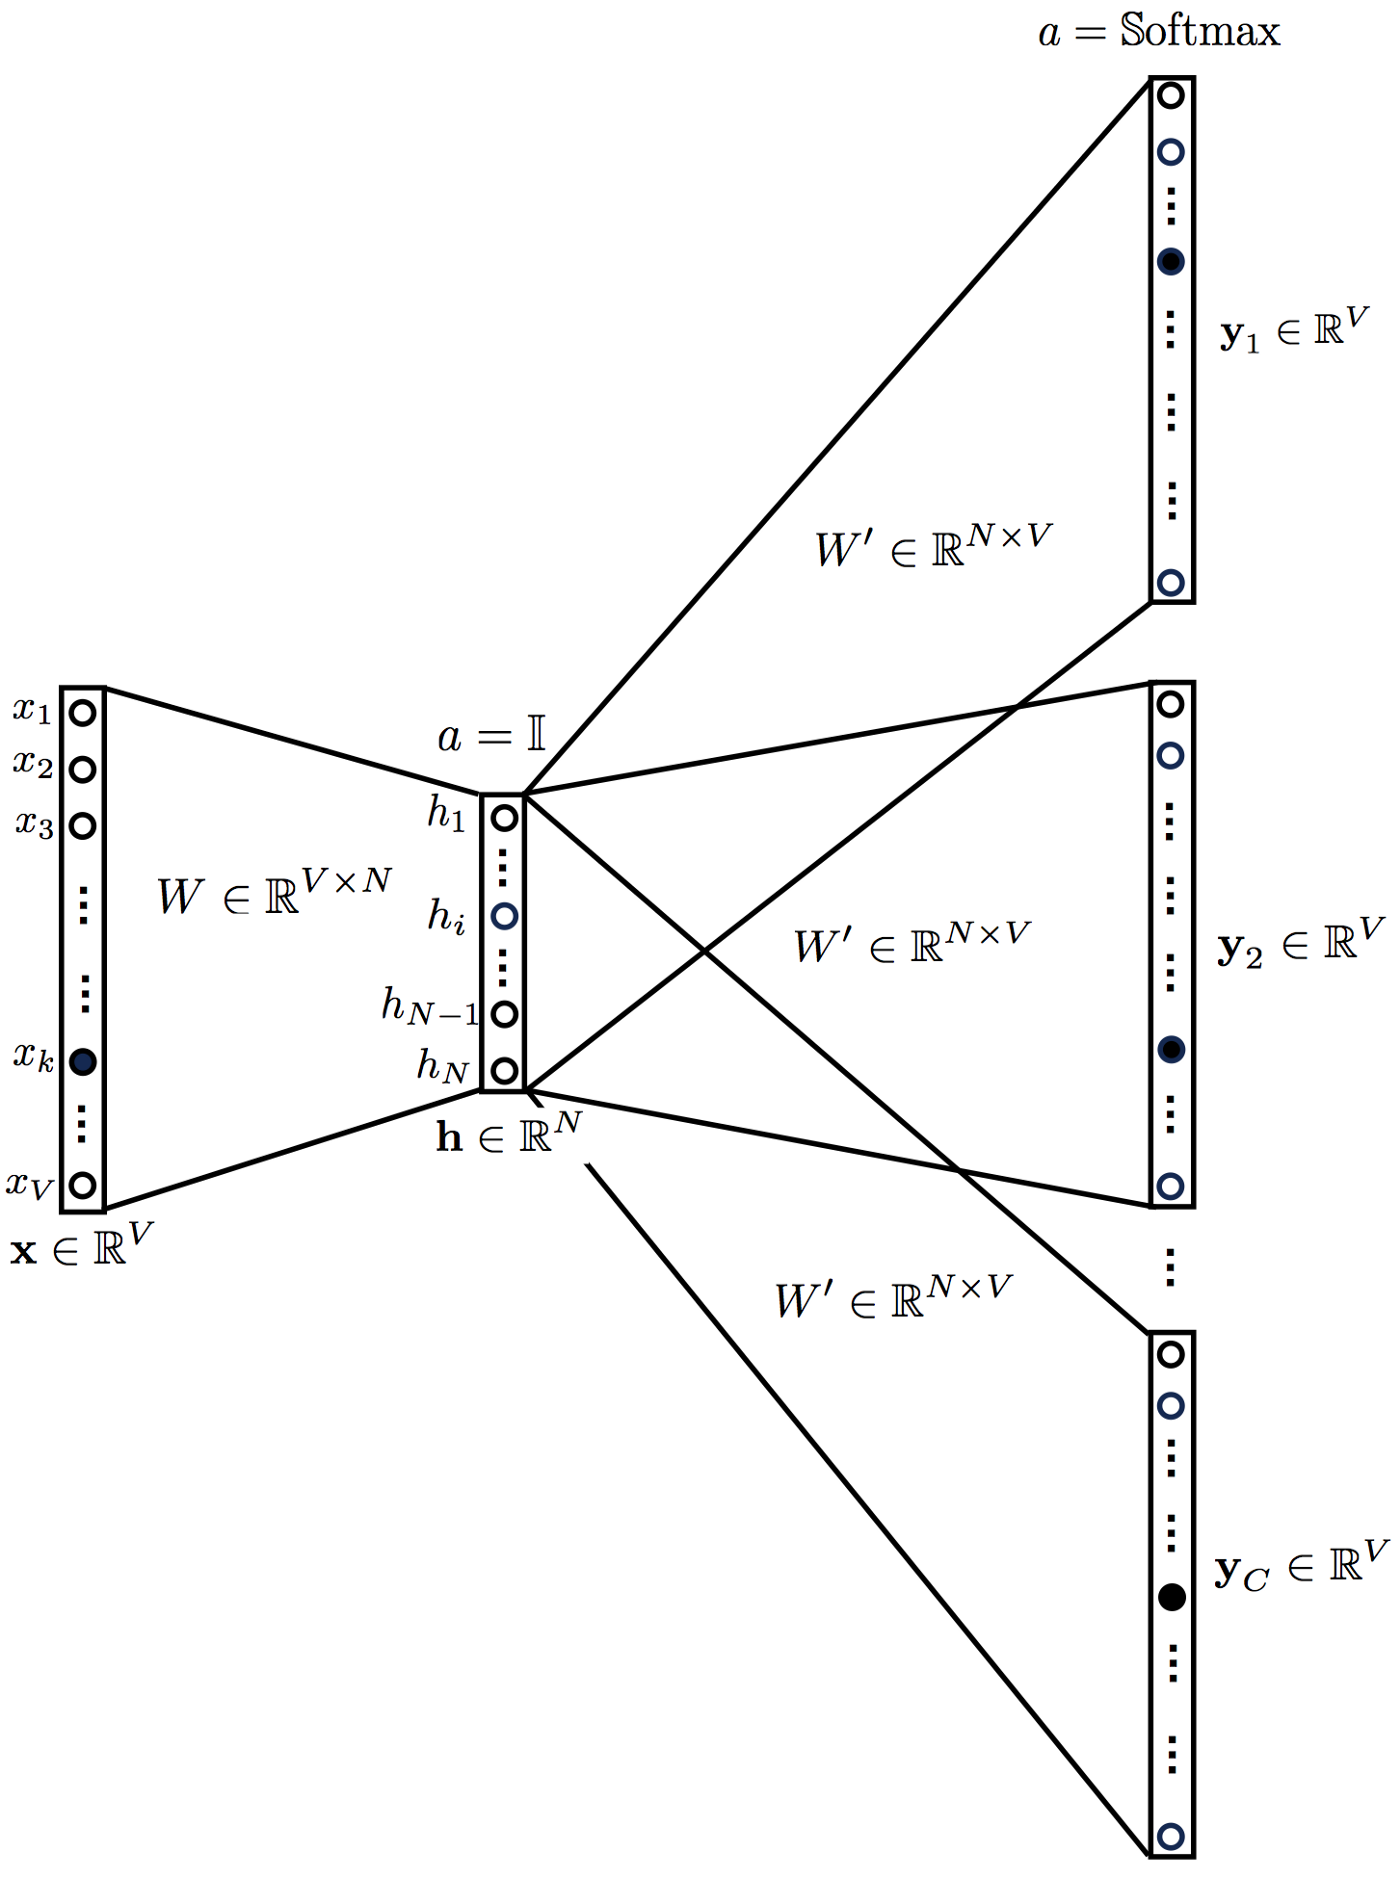
\includegraphics[width=4cm]{./images/skip.jpg}
  \label{fig:skip}
  }
  \caption{两种词向量模型\cite{mikolov2013distributed}}
  \end{figure}

\section{循环神经网络}

\subsection{RNN}

循环神经网络(RNN)是一种特殊的神经网络,其前一步的输出将作为输入输入到当前步骤\cite{zaremba2014recurrent}。在常规的神经网络中,
所有输入和输出都是彼此独立的,但是对于预测句子的下一个单词的场景下,需要前一个单词的信息作为支撑,
所以需要记住前一个单词。为解决此类问题,RNN诞生了,它借助“隐藏层”解决了这个问题。
RNN的最重要的功能是“隐藏状态”,它可以记住一些有关序列的信息。

RNN有一个“内存”,可以记住有关已计算内容的所有信息。在每一层的循环中,对输入使用相同的参数,
执行相同的任务以产生输出,这大大降低了参数的复杂性\cite{liu2016recurrent}。
虽然其他网络在前馈过程或反向传播过程中沿线性方向“行进”,但循环网络遵循循环关系而不是前馈传递,并通过使用时间反向传播进行学习。
循环神经网络由多个固定的激活功能单元组成,每个时间步长一个功能单元。
每个单元都有一个内部状态,称为单元的隐藏状态。此隐藏状态表示过去在给定时间步长上当前网络已掌握的知识,
会在每个时间步更新,以表示网络对过去的了解做出的改变。

\begin{figure}[htbp]
  \centering
  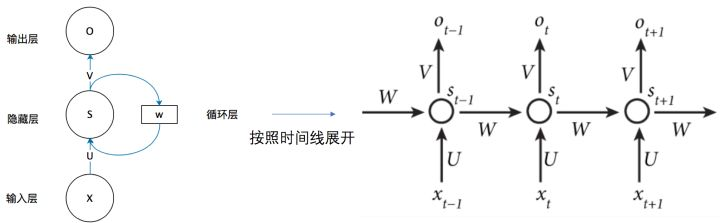
\includegraphics[scale=0.5]{./images/rnn.jpg}
  \caption{循环神经网络\cite{cho2014learning}}
  \label{fig:rnn}
\end{figure}

图\ref{fig:rnn}显示了将RNN展开为完整网络的过程,rnn可以被我们展开为我们想要的任意层数。
步骤t的输出$o_{t}$仅基于时间t的记忆进行计算,
  但是在实际情况中会有问题,因为$s_{t}$通常无法从太早时间之前捕获信息。与传统的深度神经网络在每一层使用不同的参数不同,
  RNN的参数(图中U,V,W)在所有步骤中共享。这是因为在每个步骤都执行相同的任务,只是输入的内容不同,这大大减少了需要学习的参数总数。
  % 上图在每个时间步都有输出,但是根据任务的不同,可能有些是没有必要的。例如,在预测句子的情感时,我们可能只关心最终的输出,而不关心每个单词的情感。
  % 同样,我们可能不需要每个时间步都输入。
% 例如,
% 如果输入的序列是5个单词的句子,则该网络将展开为5层神经网络,每个单词一层。对于上图具体来说,
% $x_{t}$是时刻t的输入,例如$x_{1}$ 可以是与句子的第一个单词相对应的one-hot向量。
% $s_{t}$是时刻t的隐藏状态,这是网络的“记忆”,$s_{t}$根据先前的隐藏状态和当前步骤的输入来计算

% \begin{equation}
%   s_{t}=f(U \cdot x_{t}+W \cdot s_{t-1})
%   \end{equation}

% 激活函数f通常是tanh或ReLU之类的非线性函数,$s_{-1}$计算第一个隐藏状态所需的,通常初始化为全零。
% $o_{t}$是时刻t的输出,如果我们想预测句子中的下一个单词,那么它将是整个词汇表中单词的概率分布
% \begin{equation}
%   o_t = \mathrm softmax (V \cdot s_t)
%   \end{equation}

  % 可以将隐藏状态$s_{t}$视为网络的记忆,$s_{t}$捕获有关先前时间步中发生的所有情况的信息。
  

\subsection{LSTM}
  我们在处理较简短的文本时使用RNN,往往可以取得不错的效果,这是因为此问题与语句的上下文无关,RNN不需要记住很久之前的内容。
  但是当文本长度达到一定程度时,RNN将难以驾驭。其背后的原因是梯度消失的问题,对于传统的前馈神经网络,应用于特定层的权重更新是学习率,
  上一层的误差项以及该层的输入的乘积,因此特定层的误差项是所有先前层的误差的乘积。
  通过应用经过稍微调整的RNN-长短期记忆网络,可以解决此问题。

  LSTM通过乘法和加法对信息进行了很小的修改,信息流经称为单元状态的逻辑,这样,LSTM可以有选择地记住或忘记历史信息。
  典型的LSTM网络由称为单元的不同存储块组成,其中有两种状态会转移到下一个单元格:单元状态和隐藏状态。
  内存块负责记忆事物,并通过三种主要机制(称为门)对内存进行操作。
  忘记门负责从单元状态中删除信息,LSTM不再需要了解事物的信息或重要性较低的信息将通过过滤器的乘法删除,这是优化LSTM网络性能所必需的。
  输入门负责将信息添加到单元状态,从上图可以看出,信息的添加基本上是三步过程。
  通过sigmoid函数来调节需要将哪些值添加到单元状态, 
  创建一个包含所有可能添加到单元状态的可能值的向量, 
  将sigmoid函数的值与创建的矢量(tanh函数)相乘,然后通过加法运算将此有用信息添加到单元状态。
  输出门的主要工作是将tanh函数应用于单元状态后创建矢量,从而将值缩放到-1到+1的范围, 
最后将其作为输出发送出去,到达下一个单元格的隐藏状态。
  
  \begin{figure}[htbp]
    \centering
    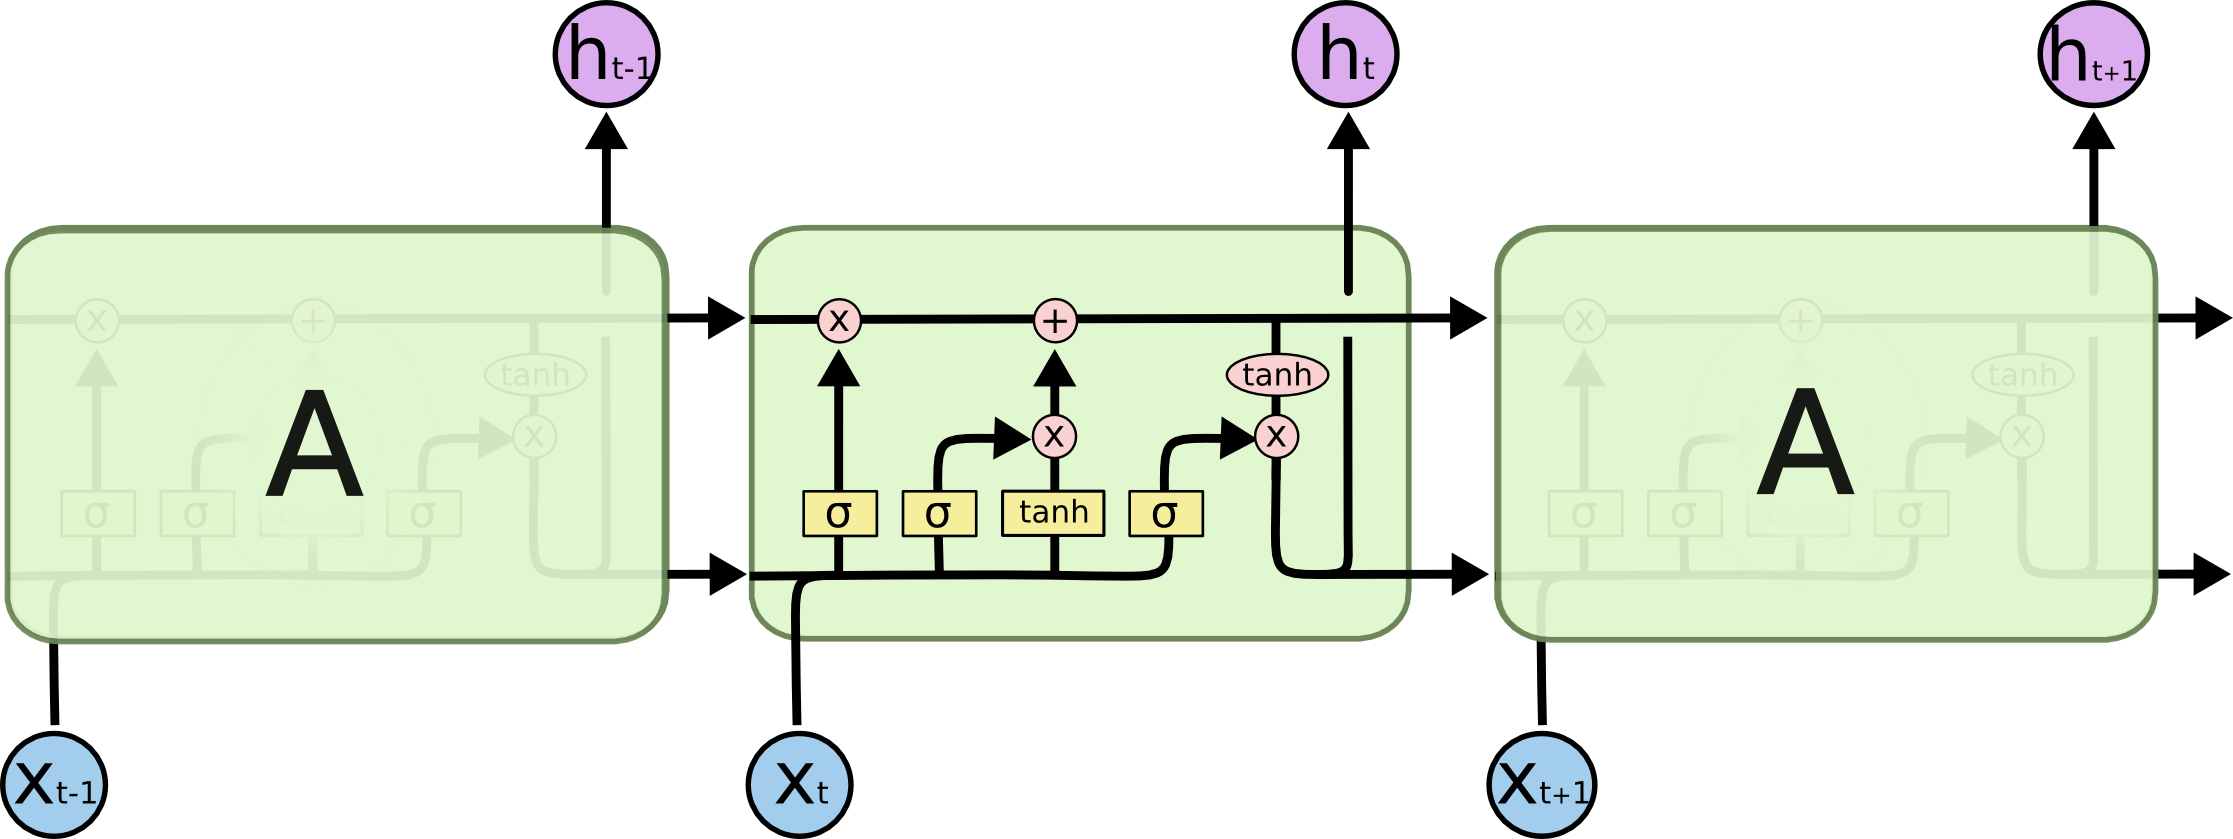
\includegraphics[scale=0.5]{./images/LSTM.jpg}
    \caption{LSTM单元模块\cite{sundermeyer2012lstm}}
    \label{fig:LSTM}
  \end{figure}
  
% \subsection{LSTM}
%   RNN的优势在于它可以将先前的信息连接到当前任务,例如使用先前的视频帧可能会有助于对当前帧的理解。
%   考虑一种语言模型,该模型试图根据前一个单词预测下一个单词。
%   如果试图预测“the clouds are in the sky”的最后一个词,则不需要任何进一步的上下文,很明显,下一个词将是“sky”,
%   在这种情况下,如果相关信息与所需信息之间的差距很小,则RNN可以很好的学习使用过去的信息。
%   但是在某些情况下,我们需要更多的上下文。考虑尝试预测文本“I grew up in France \dots I speak fluent French.”中的最后一个词,
%   最临近的信息表明,下一个词可能是一种语言的名称,但是如果想缩小哪种语言的范围,需要从更远的地方来追溯“法国”的信息。相关信息与这些相关信息被需要的地方之间的差距很大是完全可能的,
% 不幸的是随着差距的扩大RNN无法处理这一问题。

% 长短期记忆网络(通常称为“LSTM”)是一种特殊的RNN\cite{hochreiter1997long},能够学习序列的长期依赖关系,被明确设计为能够长时间记住信息的结构,
% 主要解决长序列训练过程中的梯度消失和梯度爆炸问题,它是由Hochreiter&Schmidhuber(1997)提出的,
% 并在随后的工作中被许多人改进和推广,它在各种问题上都表现出色,现已被广泛使用。
% 所有的递归神经网络都具有重复模块链的形式,在标准RNN中,此重复模块具有非常简单的结构,例如单个tanh层。
% LSTM也具有这种链状结构,但是重复模块具有与传统rnn不同的结构,它不是只有一个神经网络层,而是有四个,以非常特殊的方式进行交互。

% \begin{figure}[htbp]
%   \centering
%   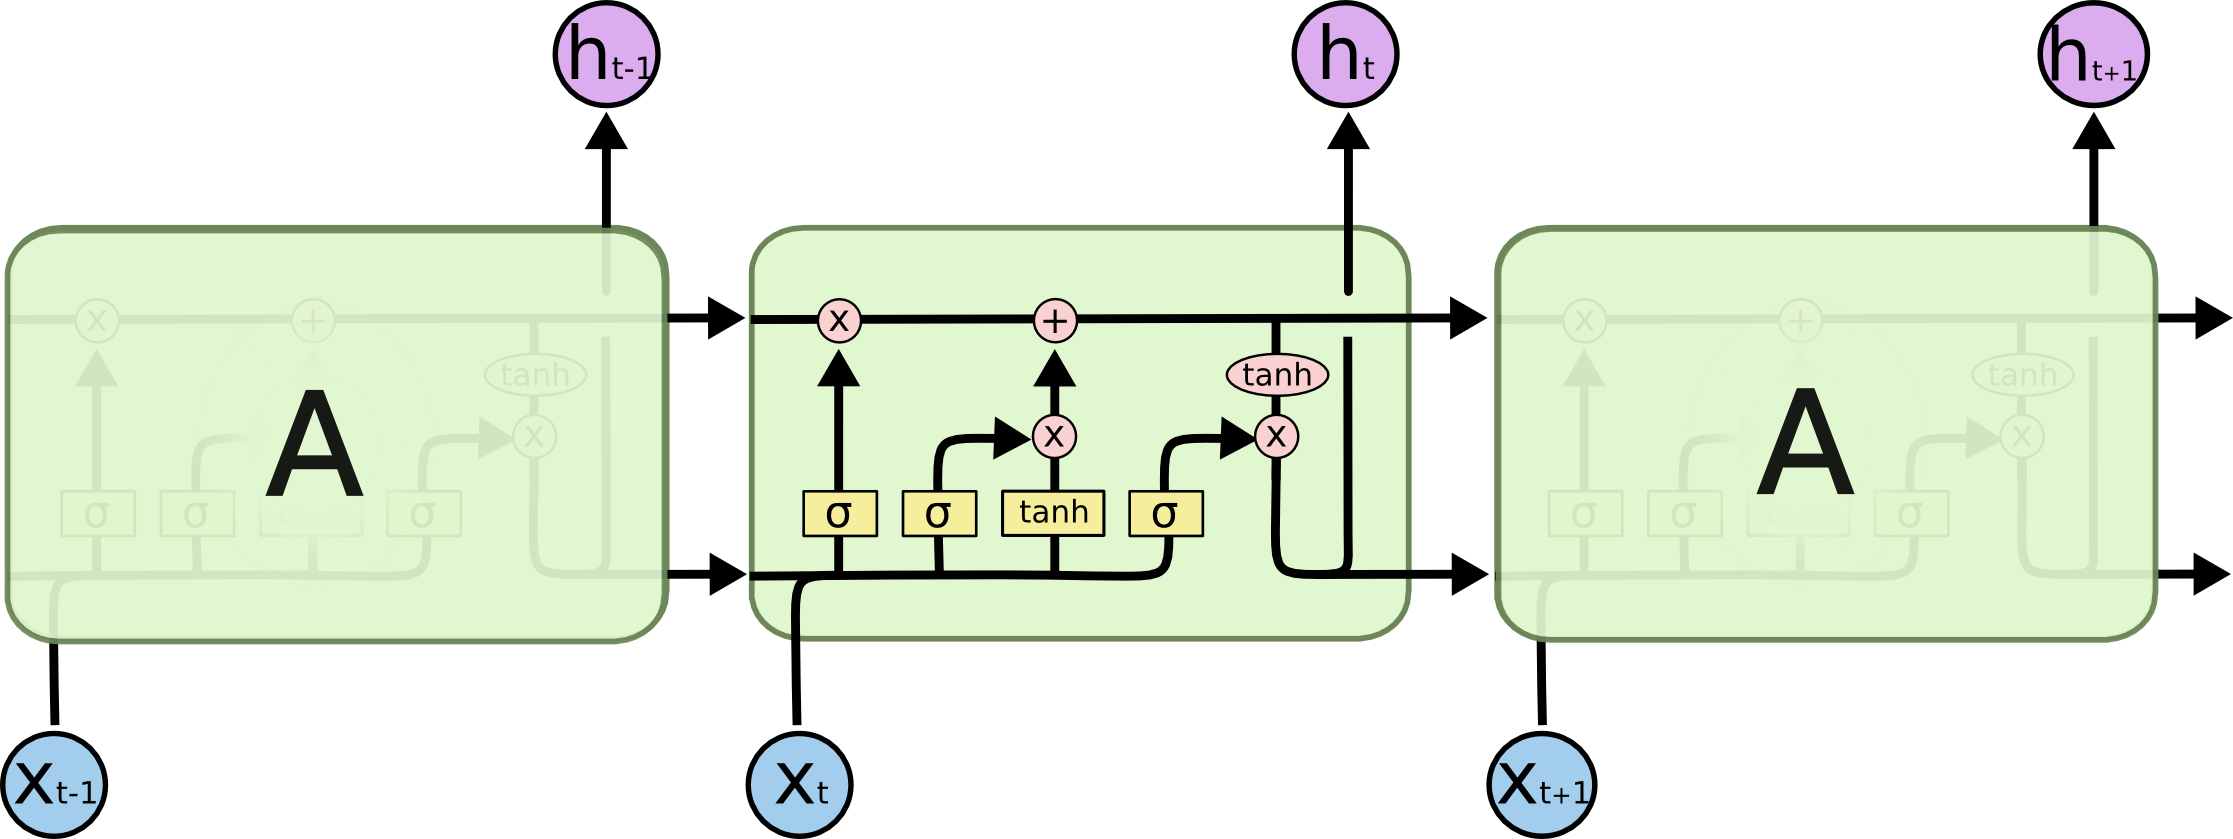
\includegraphics[scale=0.5]{./images/LSTM.jpg}
%   \caption{LSTM单元模块\cite{sundermeyer2012lstm}}
%   \label{fig:LSTM}
% \end{figure}

% LSTM结构中的关键元素是cell状态\cite{zhang2016highway},cell像传送带一样连接起来,信息流沿整个链直线传播,只有一些较小的线性相互作用,因此信息能够非常容易地不加改变地流动。
% LSTM具有删除或向单元状态添加信息的能力,这些功能由称为门的结构控制,Gates能够选择性地让信息通过,它由sigmoid神经网络层和点乘运算组成。
% sigmoid输出介于0和1之间的数字,描述应允许信息流中的多少通过。值为零表示“不让任何内容通过”,而值为1表示“让所有内容通过”。
% LSTM的第一步是确定要从单元状态中丢弃的信息,该决定由称为“遗忘门”的sigmoid层决定,它输入$h_{t-1}$和$x_{t}$,并对单元格$c_{t-1}$状态中的每个数字输出一个介于 0 和 1的值,
% 1表示“完全保留”,而0表示“完全遗忘”:
% \begin{equation}
%   f_{t}=σ(W_{f}\cdot[h_{t-1},x_t]+b_{f})
%   \end{equation}

%   下一步是确定要在cell状态下存储哪些新信息,这包括两个部分。首先,一个称为“输入门”的sigmoid层决定了我们将更新哪些值。
%   接下来,tanh层创建一个新候选值的向量$\tilde{C}_{t}$,可以将其添加到状态中。之后,我们将两者结合起来以进行状态更新:
%   \begin{equation}
%     i_{t} =\sigma\left(W_{i} \cdot\left[h_{t-1}, x_{t}\right]+b_{i}\right) 
%   \end{equation}  
%     \begin{equation}
%       \tilde{C}_{t} =\tanh \left(W_{C} \cdot\left[h_{t-1}, x_{t}\right]+b_{C}\right)
%       \end{equation}   

% 然后需要更新旧单元格状态$C_{t-1}$并得到新的单元状态$C_{t}$,前面的步骤已经确定了要做什么,只需要执行即可。
% 将旧状态乘以 $f_{t}$,让模型忘记决定忘记的信息,然后添加$i_{t} * \tilde{C}_{t}$,这是新的候选值,
% 根据此决定我们更新每个状态值的大小。
% \begin{equation}
% C_{t}=f_{t} \cdot C_{t-1}+i_{t} \cdot \tilde{C}_{t}
% \end{equation} 

% 最后需要决定要输出的内容,输出的值将基于过滤后的cell状态。
% 首先通过一个sigmoid层决定要输出单元状态的哪些部分,
% 然后通过tanh乘以sigmoid层的输出得到最终的结果,即前文提到的隐层状态$h_{t}$。
% \begin{equation}
%   o_{t}=\sigma\left(W_{o}\left[h_{t-1}, x_{t}\right]+b_{o}\right)
% \end{equation} 
% \begin{equation}
%   h_{t}=o_{t} \cdot \tanh \left(C_{t}\right)
% \end{equation}


\section{注意力机制}
注意力机制是深度学习领域中最强大的理念之一,它基于一种常识性的直觉,即我们在处理大量信息时会“关注”某个部分,这个简单而强大的概念不仅在自然语言处理任务上带来了许多突破,
还包括推荐、图像处理和语音识别等。

许多文本信息采用序列格式,例如单词、句子和文档。Seq2Seq是一个分为两部分的深度学习架构,用于将序列输入映射到序列输出,
最初是针对机器翻译任务而提出的,但可将其应用于其他序列到序列的映射任务,例如问题检索。
但是,Seq2Seq架构的潜在问题是,某些信息可能无法通过固定长度的矢量(即编码器的最终隐藏状态)捕获。
在处理长句子时,由于梯度爆炸等原因,RNN无法将足够的信息传送到句子的末尾,这会成为问题。
因此,Bahdanau等\cite{bahdanau2014neural}提出注意力机制,对机器翻译这一任务,循环神经网络每一个步长输出时,都会将上下文向量和所有词汇做语义相似度的计算得到每个词汇的权值(注意力权值),
将所有词汇按权值计算加权和得到融入注意力的输入表示,这样计算的原理是翻译结果输出的词受输入的各个词汇影响不同,通过注意力权值来显式建模这种影响程度。
直观上attention机制使与解码层输出相关性的高的输入权值更高,从而使模型达到更好的性能。

self-attention\ref{fig:attent}是attention的变种,适用于文本分类等场景,通过计算序列中的当前词和所有其他词的相似度进而得到与当前词相关的上下文向量,
用上下文向量代替原有输入向量做后续的处理。
自注意力机制允许输入彼此交互“自我”并找出他们应该更多关注的对象,输出是这些交互作用下注意力得分的加权和。
\begin{figure}[htbp]
  \centering
  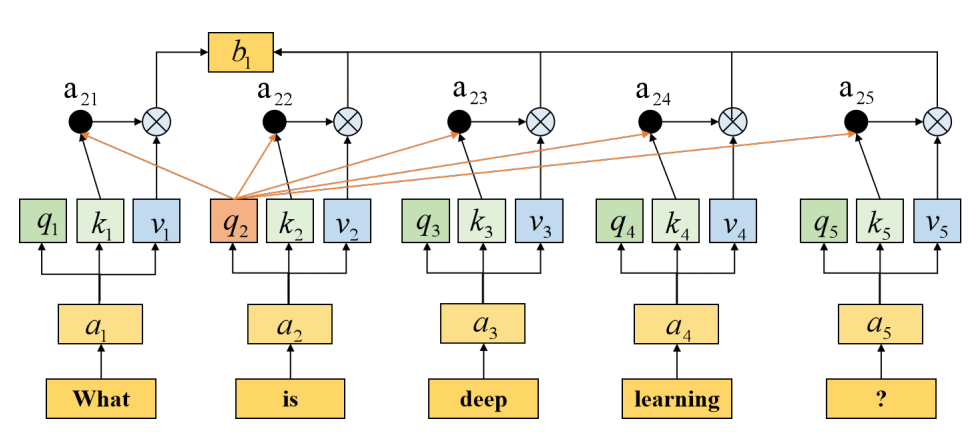
\includegraphics[width=13cm]{./images/attention.png}
  \caption{self-attention机制\cite{li2020survey}}
  \label{fig:attent}
\end{figure}

\section{transformer}
Transformer\cite{vaswani2017attention}是一种新颖的用于文本处理的架构,它使用了之前提到的注意力机制。
像RNN一样,Transformer也通过两个部分(编码器和解码器)将一个序列转换为另一个序列,
但它与先前的序列到序列模型不同,因为它并不包含任何递归神经网络网络(如GRU,LSTM等)。
在Transformer提出以前,循环网络是捕获序列中依存关系的最佳方法。 
但是,有研究表明,仅具有注意力机制而没有任何RNN(递归神经网络)的体系结构可以提升翻译任务的结果,
Transformer的提出者用BERT验证了这一点。

\begin{figure}[htbp]
  \centering
  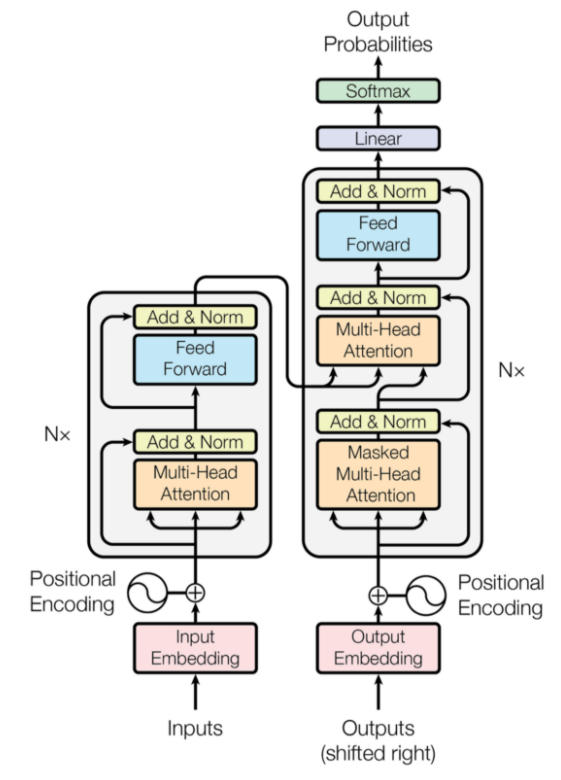
\includegraphics[width=6cm]{./images/transformer.png}
  \caption{transformer架构图\cite{vaswani2017attention}}
  \label{fig:transformer}
\end{figure}

如图\ref{fig:transformer},编码器在图中左侧,解码器在图中右侧。 
编码器和解码器均由可以相互堆叠多次的模块组成,在图中用$N_x$描述。 
编码器和解码器均主要由多头注意力和前馈神经网络组成,输入和输出(目标语句)被嵌入到n维空间中。
Transformer的一个微小但重要的改进是加入了单词的位置编码:由于Transformer没有可以记住序列位置的循环神经网络,
因此我们需要以某种方式赋予序列中的每个单词位置信息,因为顺序信息对序列文本至关重要,
这些位置信息将添加到每个单词的嵌入表示形式(n维向量)中。

\section{预训练模型}
NLP的最大挑战之一是缺乏足够的训练数据,从全局资源来看有大量的文本数据可用,但是如果对于特定任务的数据集,
最终仅能得到数千或数万个有标记的数据。不幸的是为了表现良好,基于深度学习的模型需要大量的数据,在上千万或上亿的带标注的训练样本上进行训练时,
模型效果相比少数据量会有质的提升。为了帮助弥合数据鸿沟,nlp科学家开发了多种技术,可在公开数据集中使用大量无标签的文本数据来训练通用的自然语言表示模型,
然后,可以在特定任务的较小数据集上微调这些通用的预训练模型。与从头开始对较小的特定任务的数据集进行训练相比,
预训练模型方法可显着提高准确性。BERT\cite{devlin2018bert}是这些技术中用于NLP预训练的最新应用,在深度学习社区引起了轰动,因为它在各种NLP任务中都达到了最优异的成果。

预训练模型语言建模的任务是根据上下文“填补空白”\cite{marcelino2018transfer},例如,给定
“The woman went to the store and bought a( )of shoes”,模型可能会判定“cart”一词在20%的情况合适,而“pair”一词在80%的情况合适。
在BERT之前,语言模型会在训练期间从左到右或从左到右和从右到左组合查看文本序列。这种单向方法很适合生成句子,即预测下一个单词,
将其附加到序列中,然后预测再下一个单词,直到获得完整的句子。
BERT并没有预测序列中的下一个单词,而是使用了一种称为Masked LM(MLM)的新颖技术:它随机屏蔽句子中的单词,然后尝试预测它们。
掩蔽意味着该模型是无方向性,并且与之前的语言模型不同它使用句子的整个上下文来预测被掩盖的单词。

% 预训练的语言表示可以是上下文无关或上下文相关的,上下文相关的模型又可以分为单向和双向的。
% word2vec之类的上下文无关模型会为词汇表中的每个单词生成唯一的单词嵌入表示。
% 例如,单词“bank”在“bank account”和“bank of the river”中将具有相同的向量表示。
% 另一方面,基于上下文的模型会基于句子中的其他单词生成每个单词的表示形式。例如,在句子“I accessed the bank account”,
% 单向上下文模型将基于“I accessed the”而不是“account”来表示“bank”。但是,BERT从前部和后部上下文信息(“I accessed the … account”)表示“bank”,
% 它从深度神经网络的最底层开始,使其深度双向化。

BERT依赖于Transformer,一个基本的Transformer由一个读取文本输入的编码器和一个对任务进行预测的解码器组成。
BERT编码器的输入是一系列token,这些token首先被转换为矢量,然后在神经网络中进行处理。
但是在开始处理之前,BERT需要对输入进行处理并用一些额外的元数据修饰:

1.令牌嵌入:[CLS]令牌、[SEP]令牌分别加入句子的开头和末尾。

2.段嵌入:为使编码器能够区分输入属于哪个句子加入特别的标记。

3.位置嵌入:自注意力缺少了词在句子中的位置信息,需要引入pos信息做特别标注。
\begin{figure}[htbp]
  \centering
  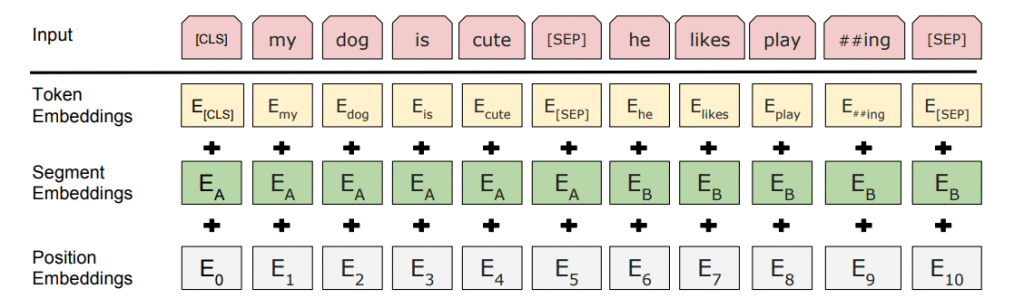
\includegraphics[scale=0.5]{./images/inputBert.jpg}
  \caption{BERT的输入处理\cite{devlin2018bert}}
  \label{fig:inputBert}
\end{figure}

BERT不会尝试预测句子中的下一个单词,训练时使用以下两种策略:

Masked LM (MLM),
随机掩盖输入中15%的单词(用[MASK]令牌代替),将处理好的序列输入模型,然后根据序列中其他未屏蔽单词提供的上下文信息预测被屏蔽的词,
但是,这种掩盖方法存在一个问题,模型只会预测输入中存在的词,而我们希望模型尝试预测正确的token,而不管该token是否存在于输入中。
要解决此问题,BERT在训练时,对于被选中要被屏蔽的词,有80%按原方案被替换为令牌[MASK],10%被替换为随机token,剩下10%保持不变。

Next Sentence Prediction,
为了理解两个句子之间的关系,BERT训练过程还进行了下一个句子预测,具有这种理解的预训练模型可以解决诸如回答问题之类的任务。
在训练过程中,该模型将句子对作为输入,并学习预测第二个句子是否是原始文本中的下一个句子。第二句出现在第一句之后的概率有50%,剩下50%出现的是语料库中随机的句子。

\section{本章小结}
本章介绍了智能服务调用语义理解任务需要用到的nlp相关技术,词向量技术包括CBOW和skip-gram两种,循环神经网络主要讨论了RNN和LSTM,
介绍了近年来深度学习领域较为火热的注意力机制,最后讨论了最近在nlp领域的新技术transformer和预训练模型BERT。

% \chapter{基于深度学习的用户语义理解}

\section{语义理解任务描述与解决流程}
\subsection{问题描述}
跨界服务平台内服务的智能调用实现过程中,语义理解是关键。系统接收的是用户输入的一句有目的性的话,系统在语义理解的过程中,
首先要识别用户的意图,根据
用户意图匹配相应的服务以及匹配该服务要执行的操作,这两者均可被视为文本分类问题,可以用深度学习的分类算法解决,
再本文被称作服务分类和接口分类任务;找到匹配的服务以后,在服务执行前
必要的执行参数,可以从用户输入的语句中提取,这将被看作语义槽填充问题,可以用序列标注算法解决,
将词语序列x=[$x_{1}$,$x_{2}$,\dots,$x_{T}$]映射到相应的插槽标签序列y=[$y_{1}$,$y_{2}$,\dots,$y_{T}$],再本文被称作参数提取任务。

以调用火车票信息查询服务为例,来解释跨界服务平台内服务分类,接口分类和参数提取。
用户在进入跨界服务平台后,输入“查询成都前往杭州的火车票”,跨界服务平台内
的语义理解模型识别出该语义对应平台内部的<train服务>,接口类型为<query查询>,语义槽(即服务参数)为<startCity起始地>成都和<endCity目的地>杭州。


\begin{figure}[htbp]
    \centering
    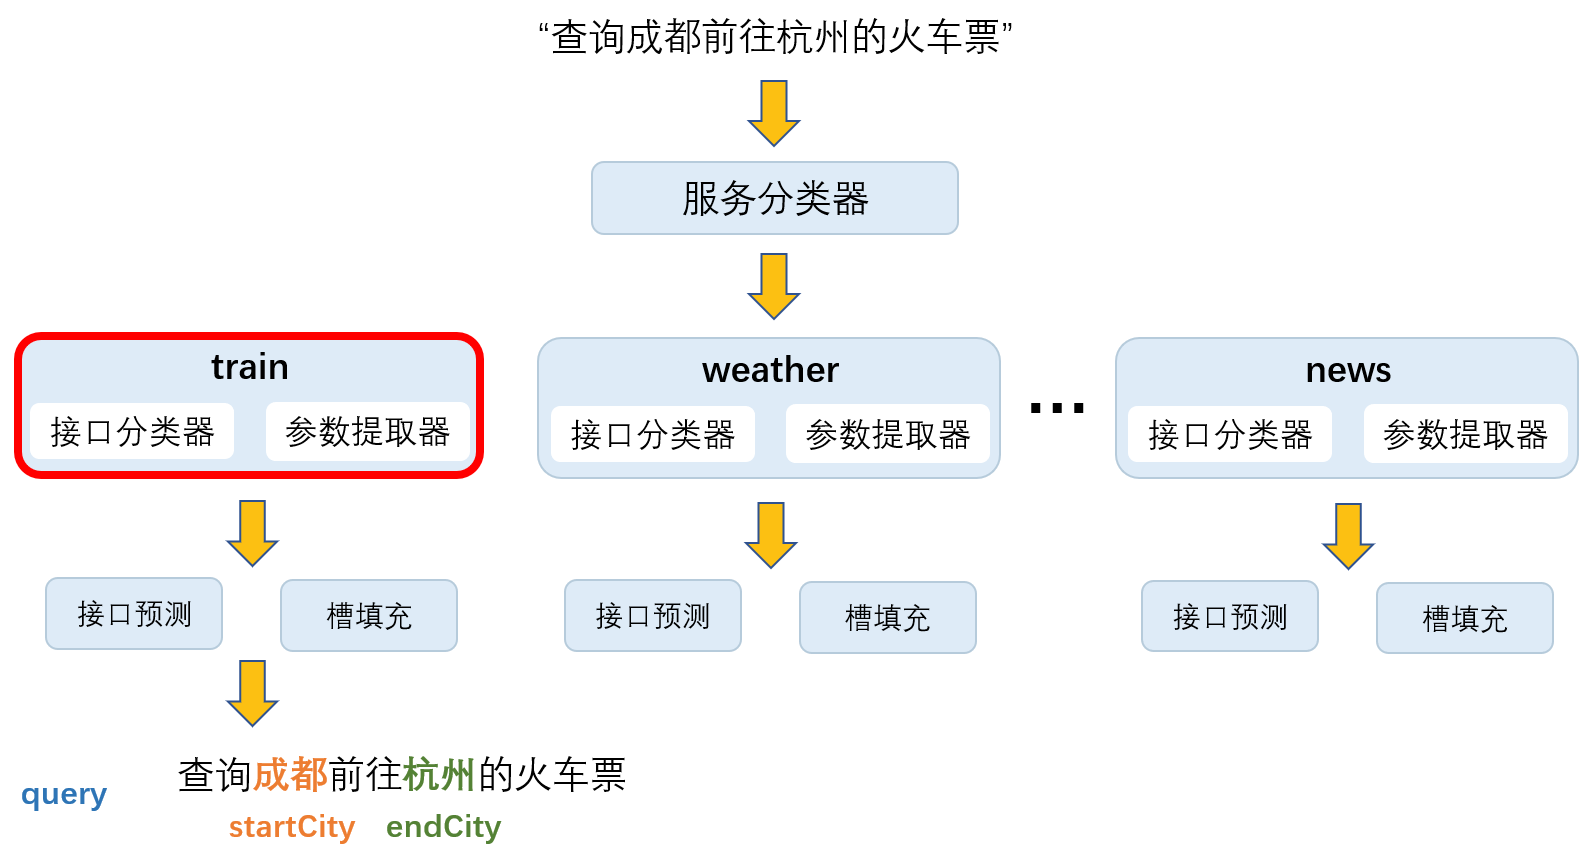
\includegraphics[scale=0.5]{./images/liucheng.png}
    \caption{语义理解算法流程}
    \label{fig:questiondesc}
  \end{figure}

\subsection{算法描述}
基于深度学习的语义理解算法,首先将用户输入的句子利用分词工具转化为词语序列,再用word2vec将词语向量化,
固定句子长度后,得到结构化的表示形式x=[$x_{1}$,$x_{2}$,\dots,$x_{T}$]输入网络中,流程如图\ref{fig:questiondesc}所示。
首先利用服务分类器得到系统内与用户意图相匹配的服务,再通过接口分类器和参数提取器分别做文本分类和语义槽填充处理,最后将三项任务得到
的结果提交至服务执行引擎做服务调用,算法详细描述如表\ref{tab:suanfa1}。

\begin{table}[htb]
  \centering
  \caption{基于深度学习的语义理解算法描述}
  \label{tab:suanfa1}
\begin{tabular}{p{150mm}}
\toprule
\textbf{算法1:}基于深度学习的语义理解\\
\textbf{输入:} $L_0$=\{($S_i$,$y_i^d$,$y_i^i$,$y_i^s$)\},i $\in$ [1,n]\\
\textbf{输出:} $Model_{service}$,$Model_{interface}$,$Model_{slot}$\\
\hline
\textbf{过程描述:}模型在训练时,输入的$S_i$为有用户意图的语句,经过分词和向量化
处理后得到$E_i=(e_1,e_2,\dots,e_T)$,T为词语个数。模型参数初始化、批处理的数量
iterations = M 和每一批的样本数 batchsize、迭代次数 epoch = N 和当前迭代次数 i = 0\\
\textbf{while} i < N or 模型的性能达到终止条件 \textbf{do}\\
\qquad \qquad \textbf{for} j = 1,\dots ,M \textbf{do}\\
\qquad \qquad \qquad \qquad 随机抽取 batchsize 个训练集数据,前向传输在当前网络权值和输入下网络的输出\\
\qquad \qquad \qquad \qquad 反向传输调整模型参数\\
\qquad \qquad \textbf{end for}\\
\qquad \qquad 计算损失 Loss,更新梯度和模型的参数\\
\textbf{end while}\\
用训练好的领域分类模型对测试样本进行预测,加载训练好的相应领域的意图识别模型
和语义槽填充模型,对意图和语义槽进行预测,计算准确率 Accuracy、损失 Loss\\
\bottomrule
\end{tabular}
\end{table}

\section{预处理}
\subsection{序列化}
% 结巴分词,word2vec
% 用户不需要输入完整的句子
神经网络的输入是一个向量序列,但用户输入是一个完整的句子,因此首先需要把句子序列化,之后使用word2vec将词语向量化。
本文采用结巴分词来做序列化的处理,
结巴分词分了三种模式,准确模式试图将句子切成最贴切的句段,适用于文本分析;完全模式会从句子中获取所有可能的单词,速度快但不精确;
基于准确模式的搜索引擎模式试图将长词切成几个短词,从而提高查全率,适用于搜索引擎。
结巴分词的算法依据主要是基于前缀字典结构来实现高效的词图扫描,为所有可能的单词组合构建有向无环图(DAG),
使用动态规划根据单词频率查找最可能的组合。

本文在实际处理中发现文本的预处理特别重要,如果句子中包含了太多无关词(这些词被称作停用词),算法性能会受影响,因此本文
在文本预处理时引用了停用词过滤。比较常见的中文停用词如“的”、“在”以及语气词等,他们的存在对语义理解没有贡献,相反如果分词工具使用他们错误的分词,
会降低模型准确率,因此本文利用网上已有的中文停用词词典在结巴分词工具处理前对用户语句做了停用词过滤。

\subsection{标签向量化}
服务分类和接口分类均属于多类别分类问题,训练样本的标签均采用one-hot编码,本文筛选了跨界服务平台中用户使用较多的八类服务,接口类型为这八类
服务下所有接口的合计,如query,order,play等。对于参数提取任务,像序列标注任务一样,使用BIO标注方式标记参数语义槽,根据类型不同分为
“B-X”、“I-X”和“O”,如图\ref{fig:yuyicao}所示。
\begin{figure}[htbp]
  \centering
  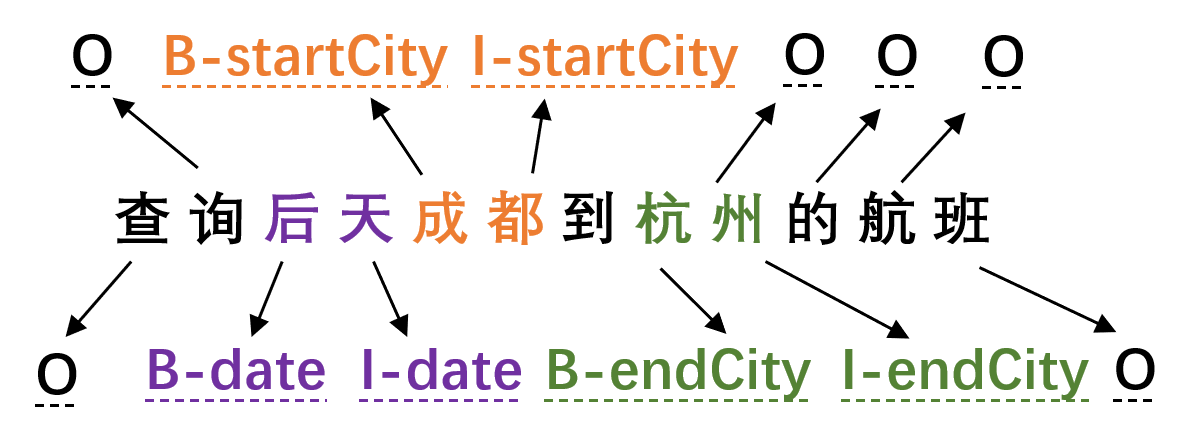
\includegraphics[scale=0.5]{./images/yuyicao.png}
  \caption{参数语义槽标注}
  \label{fig:yuyicao}
\end{figure}


\section{基于ATT-CLSTM的服务分类模型}
实现服务智能调用的第一步要根据用户意图匹配相应的服务,这可以被转化为文本分类问题。
LSTM
是一种特殊的RNN,能够学习长期依赖关系,理解关键字出现的顺序,擅长处理文本序列的问题,同时,
它通过增加门控机制来过滤信息,解决了长距离依赖的问题。 另一方面,在某种程度上也避免了梯度消失和梯度爆炸的问题。
CNN
多用于图像领域,由于卷积核的存在,能够提取出词与词之间的隐藏的语义信息,捕获局部相关性。
尽管CNN可以在许多任务中很好地表现,但它最大问题之一是卷积核大小的在训练时固定,不具有很好的泛化能力。一方面,无法对更长的序列信息进行建模,
另一方面,超参数卷积核大小的调整也增加了工作量,池化层的处理也会丢失了部分结构性信息,因此很难在文本中发现复杂的模式。
为了
能让卷积层从词嵌入向量中提取更高级的语义表示,我们在模型中引入attention层.这是因为在传统的CNN中,有效地编码长期上下文信息和非连续词之间的相关性并不容易,
它仅考虑在字符串上连续的n-gram信息,因此忽略了非连续词之间的某些长距离相关性,而这种相关性在许多语言中都起着重要作用。例如,用户输入“帮我挂
明天上午邵逸夫医院的号”,这里“挂”和“号”显然应该组合在一起成词才能具有完整正确的语义信息。NLP中有关注意力的大多数现有研究都集中在对不同模式之间的相关性进行建模,
因此在本文中,我们将attention层放在卷积层之前,
用于自动捕获长期上下文信息和非连续词之间的相关性,而无需任何外部语法信息。

综上所述本节将三者结合各取所长, 采用ATT-CLSTM模型\ref{fig:cnn-lstm}用以解决服务分类问题,下面将详细介绍该模型

\begin{figure}[htbp]
    \centering
    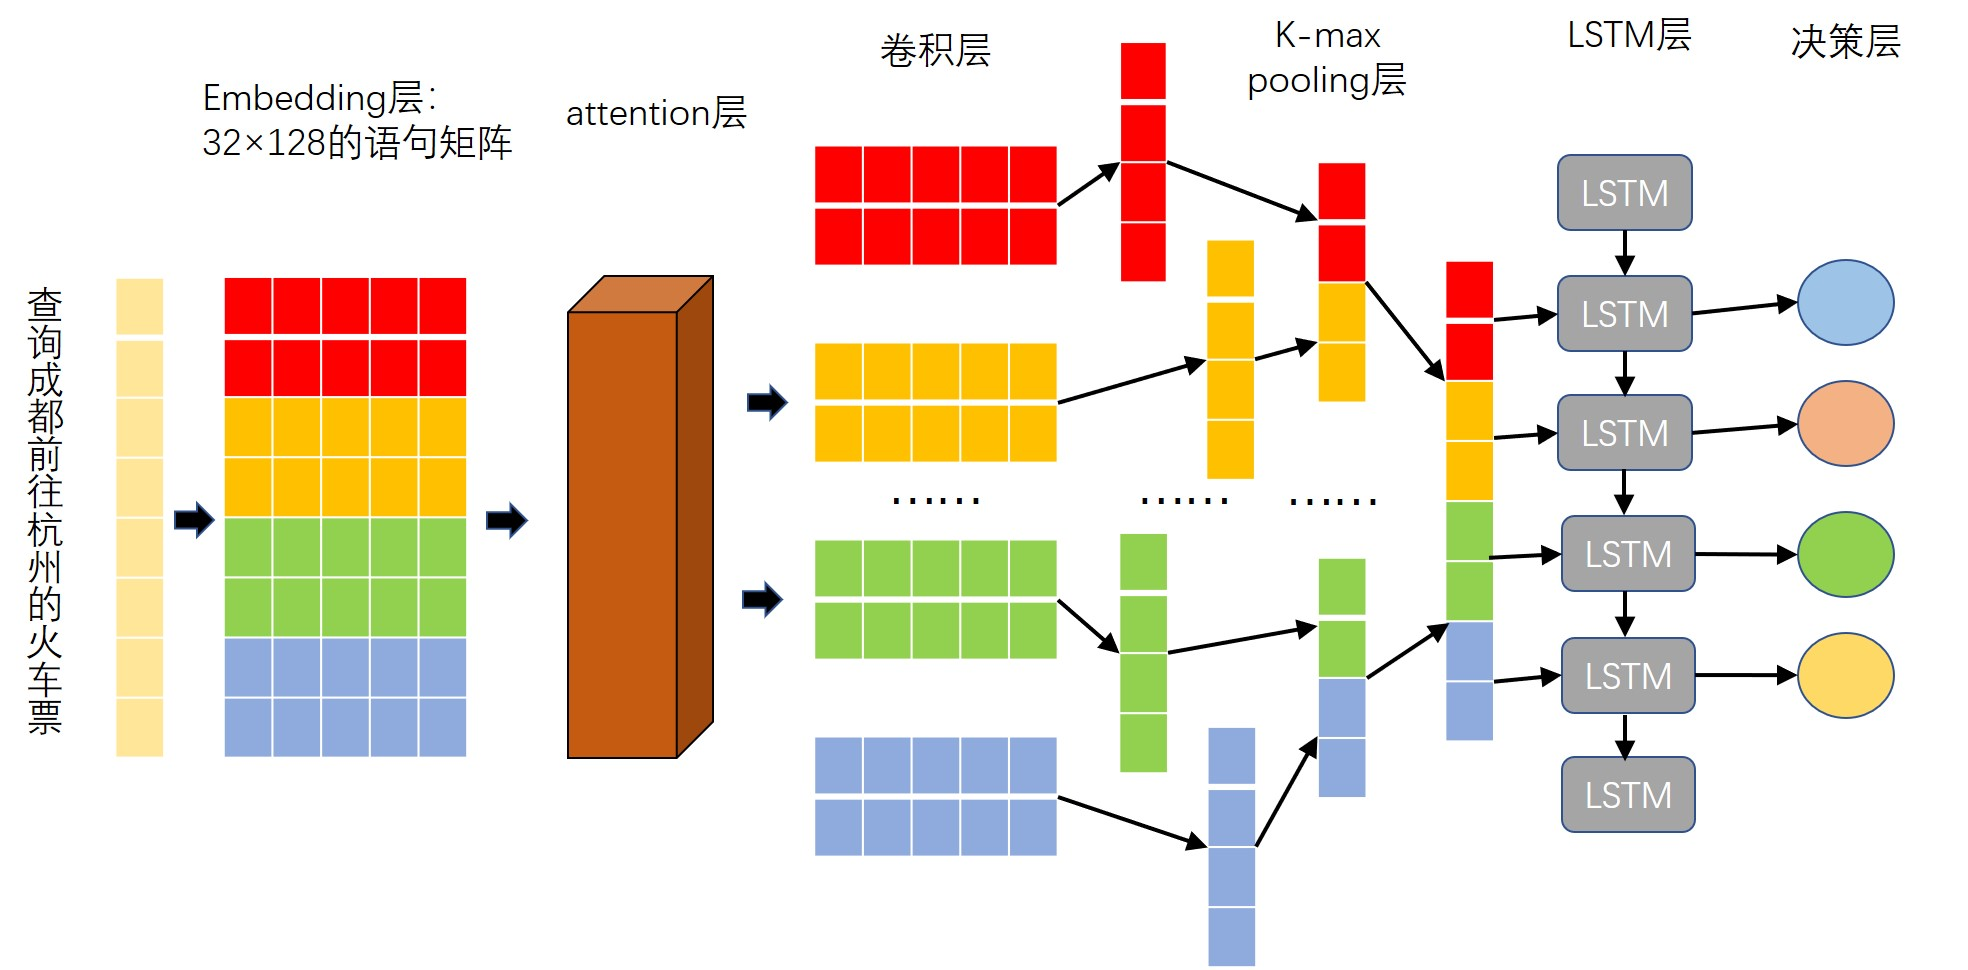
\includegraphics[scale=0.5]{./images/cnn-lstm.jpg}
    \caption{服务分类模型}
    \label{fig:cnn-lstm}
  \end{figure}


  1)输入层与embedding层

  用户输入的语句通过结巴分词工具得到中文词的模型即可完成输入层的任务到达embedding层。之后将文本序列转换为矢量形式的数字表示,word2vec是最常用的方法之一。
  在本实验中,我们选择通过C-BOW基于维基百科中文语料库预训练得到的word2vec模型,通过使用预训练词向量模型可以有效地减少人工神经网络的过拟合。
  由于神经网络的输入长度在本模型中是固定的,加之用户输入的语句长度通常有限,结合数据集中最长句子拆分以后的序列长度考量,我们决定把最大长度设为32.
  同时word2vec模型的输出的词向量维度为128维,因此每一个需要匹配系统内服务的用户输入的句子就构成了一个32×128的二维矩阵E=[$e_{1}$,$e_{2}$,\dots,$e_{32}$],
  其中$e_{i}$=[$e_{i1}$,$e_{i2}$,\dots,$e_{i128}$]是一个中文词经过word2vec处理的向量表示。

  2)attention层

  如图\ref{fig:att-cnn}所示,是注意力层的主要结构,在输入层和卷积层之间引入了注意层.具体而言,注意力层是为每个词创建上下文向量,
  上下文向量与词向量串联在一起,作为新的词表示形式将被输入到到卷积层。 
  注意机制的思想是在推导$x_{i}$的上下文向量$g_{i}$时将注意力集中在特定的重要单词上,图\ref{fig:att-cnn}中的红色矩形代表$x_{i}$的上下文向量$g_{i}$,
  这种机制确定了在预测服务类别时哪些词应比句子上的其他单词获得更多的关注。
  注意机制是一个附加的多层感知器,它与ATT-CLSTM的所有其他组件共同训练。
  注意力机制生成的上下文向量$g_{i}$由以下公式得到:
  \begin{equation}
  \mathbf{g}_{i}=\sum_{j \neq i} \alpha_{i, j} \cdot \mathbf{x}_{j}
\end{equation}
其中,$\alpha_{i, j}$是注意力权重值,其计算方式如下:
\begin{equation}
\alpha_{i, j}=\frac{\exp \left(\operatorname{score}\left(\mathbf{x}_{i}, \mathbf{x}_{j}\right)\right)}{\sum_{j^{\prime}} \exp \left(\operatorname{score}\left(\mathbf{x}_{i}, \mathbf{x}_{j^{\prime}}\right)\right)}
\end{equation}
\begin{equation}
\text { score }\left(\mathbf{x}_{i}, \mathbf{x}_{j}\right)=v_{a}^{\top} \tanh \left(W_{a}\left[\mathbf{x}_{i} \oplus \mathbf{x}_{j}\right]\right)
\end{equation}
词与词之间的score值由感知器计算得到,$v_{a},W_{a}$为MLP权重参数,以此来度量词与词之间的相关性,得分越高表示相关性越强。
经过这一层的处理,用户输入的句子被转换为32×256的二维矩阵A=[$a_{1}$,$a_{2}$,\dots,$a_{32}$],
其中$a_{i}$=[$a_{i1}$,$a_{i2}$,\dots,$a_{i256}$]是一个中文词经过attention处理的向量表示。

\begin{figure}[htbp]
  \centering
  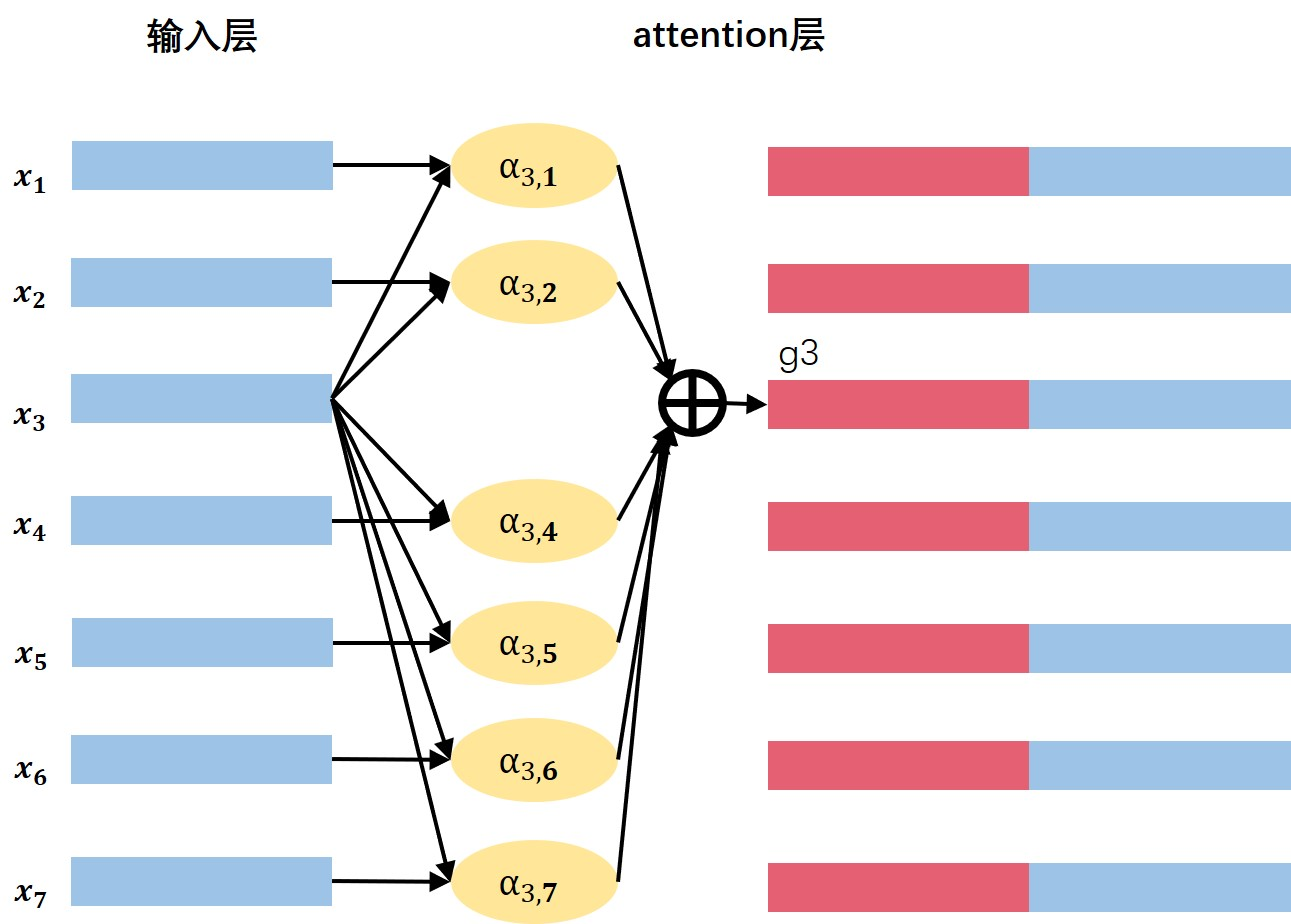
\includegraphics[scale=0.4]{./images/attcnn.jpg}
  \caption{服务分类模型中attention层}
  \label{fig:att-cnn}
\end{figure}
  3)卷积层

  由于卷积核的存在,卷积层能够提取出词与词之间的隐藏的语义信息,捕获局部相关性。这里我们仅设置了单层的卷积层,用于捕获序列局部相关信息并对输入数据的降维。
  设置不同初始化权重的多个卷积核可以提高模型的学习能力,本模型共设置了64个卷积核,卷积核在文本矩阵上移动以提取特征。在文本处理领域CNN的卷积操作常被设置
  为一维卷积,这是因为直观上来看沿着词向量所在的维度不具有拆分性,因此卷积核总是沿着词与词之间的维度扫描提取特征,对m×n的矩阵用高为h的卷积核做一维卷积
  会得到一个高为m-h+1,宽为1的长条状矩阵。基于此,本文卷积核宽度与attention输出层
  一致为256,高度设置了[2,3]两种选择以期获得不同视角的语义信息,所以本层的输出结果大小随卷积核的尺寸不同会不一致,即会得到64个大小不一的矩阵称为feature maps.
  卷积操作的计算公式如下:
  \begin{equation}
    c=ReLU(W_{c}A+b_{c})
    \end{equation}
    这里选用ReLU作为非线性激活函数,减少参数之间的相互依赖性避免梯度消失和过拟合等问题,c为一个卷积核做一次卷积运算所得值。

  4)pooling层

    如上层所述,卷积层的输出结果大小随卷积核的尺寸不同会不一致,因此池化层有统一维度的作用,
    同时可以降维降低计算复杂度,保留核心特征,减少模型参数防止过拟合提高模型泛化能力。
    由于卷积核卷积操作得到的结果是长条状,因此本文采用k-max pooling池化方法,k是超参数,经实验调整为4。
    经过池化层处理后,得到4×64的特征矩阵作为lstm层的输入。
    从64维的角度来看,每一维是一种高层语义特征的提取。

    5)lstm层

  直观上,文本分类是顺序信息处理的过程。但是,从卷积神经网络以并行方式获得的特征序列不包含序列信息,LSTM专为顺序建模而设计,
  可以进一步从CNN获得的特征序列中提取上下文信息,lstm内部核心计算过程如下:
  \begin{equation}
  f_{t}=σ(W_{f}\cdot[h_{t-1},x_t]+b_{f})
  \end{equation}
  \begin{equation}
    C_{t}=f_{t} * C_{t-1}+i_{t} * \tilde{C}_{t}
    \end{equation} 
    \begin{equation}
      o_{t}=\sigma\left(W_{o}\left[h_{t-1}, x_{t}\right]+b_{o}\right)
    \end{equation} 
    \begin{equation}
      h_{t}=o_{t} * \tanh \left(C_{t}\right)
    \end{equation}
    其中,$x_t$为从池化层输入的变量,其他字符代表的是lstm内部计算的中间过程变量不再赘述,得到的所有隐层信息$h_t$被输入到下一层
  6)优化层与决策层
    由于本模型层度较深参数较多,为防止训练时发生过拟合,在lstm层后接入dropout(未在图中表示),最后利用softmax做分类决策。

实验结果表明,矩阵分别经过注意力卷积层和LSTM层后,可以获得较高程度提取的语义信息。



\section{基于Trans-CLSTM的接口分类模型}
接口分类和服务分类本质上一样都可以视为文本分类问题,我们在处理接口分类问题时没有生搬硬套服务分类模型,
而是希望改进以提升性能,因此做了不同的尝试,以期寻找到最适合跨界服务领域的文本分类模型。
CNN在许多自然语言处理任务中都很有效,由于常规的CNN具有许多几何上固定的结构 ,CNN不可避免地面临适应非规则形状特征的挑战。
例如卷积层将卷积层形状限制为n-gram,而pooling层会使用solid chunks提取高层语义特征,
这些固定的结构为语义表示带来了两个限制:所有卷积核和块都是连续的且形状固定的,
这使CNN难以处理某些复杂的情况,例如非连续或过大的特征,换句话说,它处理不了不符合卷积核形状的特征,并且传统的CNN无法主动进行调整以适应特征的转换。
在训练中他们倾向于记住数据集中各种形式的特征,但不了解这些特征的经过变换以后的形状。举个例子,
给定短语“不那么好”,传统的卷积网络很难直接捕获非连续特征“不...好”,也很难从其他变换形式中识别出,例如“不太好”,这些均为“不好”这个特征的变换形式。

本节采用了端到端的文本分类模块,修改了卷积神经网络中的传统卷积层,称作可变换卷积层,该模块可以增强CNN对变换特征的捕捉和建模能力。
可变换卷积引入位置偏差信息$\Delta p$的概念,将位置偏差信息$\Delta p$添加到卷积核的采样位置,
这样卷积核的采样位置会因为$\Delta p$而变化,达到捕获复杂特征的目的。
$\Delta p$被设计为神经网络自动学习,而无需额外的信息或人工监督。
同时由于lstm能够学习长期依赖关系,理解关键字出现的顺序,擅长处理文本序列的问题.我们把lstm拼接在池化层之后对语义信息做进一步的处理,
接口分类的模型如图\ref{fig:tran-cnn-lstm},下面将详细介绍该模型:

\begin{figure}[htbp]
  \centering
  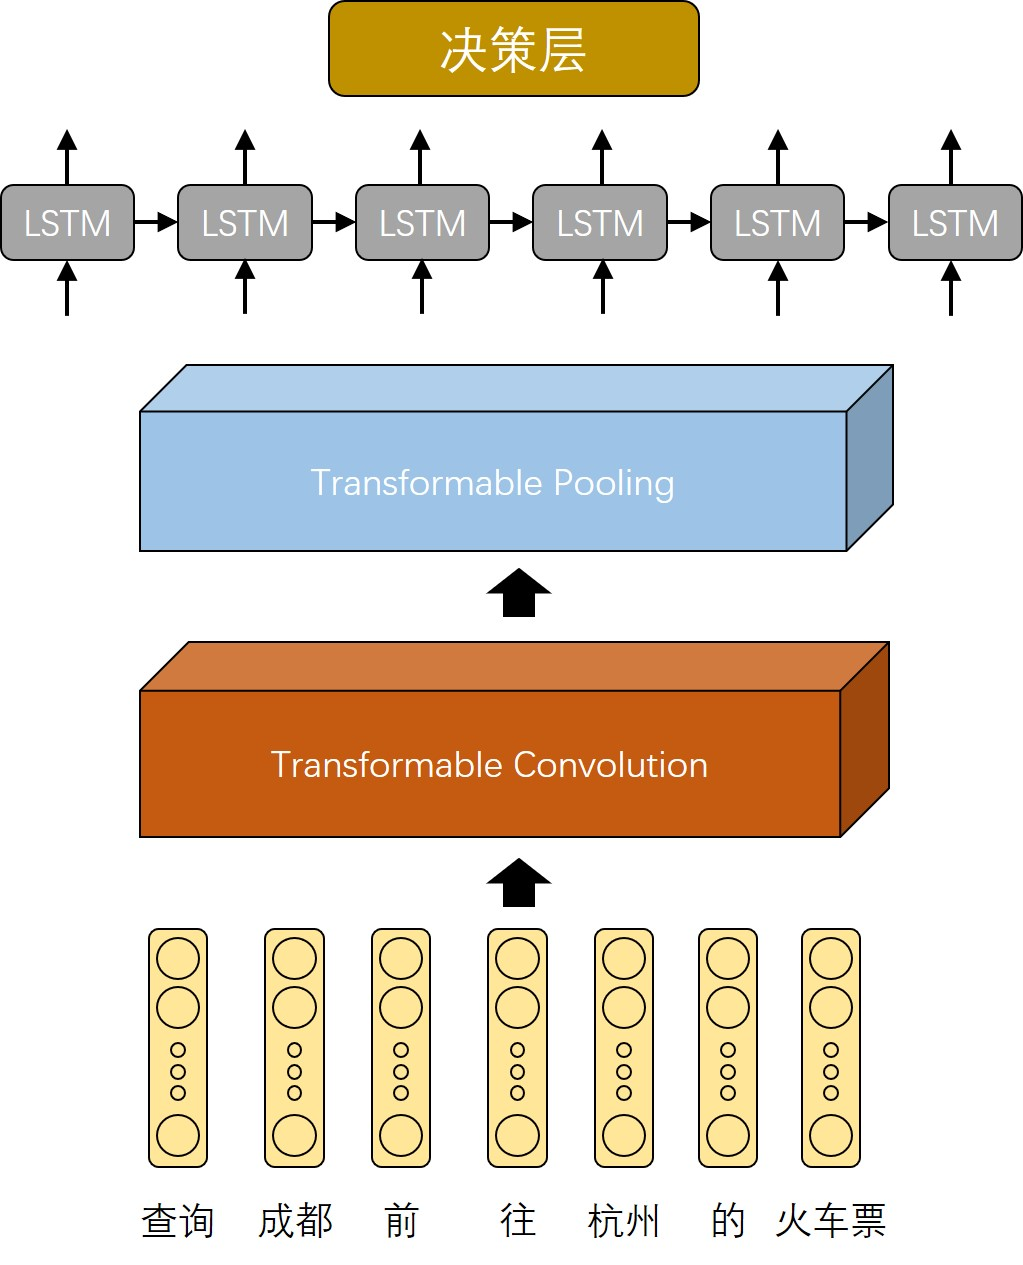
\includegraphics[scale=0.4]{./images/tran-cnn-lstm.jpg}
  \caption{接口分类模型}
  \label{fig:tran-cnn-lstm}
\end{figure}

1)输入层与embedding层

该层与服务分类模型做相同处理,不再赘述。需要注意的是与服务分类模型有一处不同,我们选择输出维度为256维的词向量模型,序列长度仍为32,
因此每一个需要匹配系统内服务的用户输入的句子就构成了一个32×256的二维矩阵E=[$e_{1}$,$e_{2}$,\dots,$e_{32}$],
其中$e_{i}$=[$e_{i1}$,$e_{i2}$,\dots,$e_{i256}$]是一个中文词经过word2vec处理的向量表示。


2)可变换卷积层

可变换卷积层是本模型的核心模块,该模块具有可学习的形状以适应特征的变化。 
通常,卷积核的形状因为是超参数从一开始就是固定的,但是可变换模块将学习到的位置偏差信息添加到卷积核上,从而使其形状灵活,特征变换适应性增强。 
位置偏差信息由动态部分和静态部分组成,在预测阶段,动态偏差与当前输入有关,其值可从当前输入中经过计算主动获取以捕获特征变换信息。 
相反,静态偏差值像其他权值一样通过反向传播进行更新,并在预测阶段保持不变,这描述了模型从训练集中学到的特征信息的基本分布。
对于传统CNN的卷积核大小是固定,卷积核在对输入图像扫描过程中每一次卷积操作的范围是固定的,如图\ref{fig:tansconv}的左图所示,一次普通的卷积运算可以用以下公式表示:
\begin{equation}
  y=\mathbf{w}\mathbf{x}
  \end{equation}
  将上式展开计算卷积核中每一个元素,公式被转换为:
  \begin{equation}
    \mathbf{y}\left(p_{0}\right)=\sum_{p_{i} \in \mathbf{C}} \mathbf{w}\left(p_{i}\right) \cdot \mathbf{x}\left(p_{0}+p_{i}\right)
    \end{equation}
其中,C为本次卷积核采样的全集,$p_{0}$是卷积运算后本次卷积在结果特征图中的位置,$p_{i}$枚举了本次卷积核采样的全集中的所有位置,并且
表示与$p_{0}$的距离。

在可变换卷积(transformable convolution)中,一次卷积运算的采样全集C被分为两部分,分别用$\mathbf{D}_{c} \subset \mathbf{C}$和
$\mathbf{S}_{c} \subset \mathbf{C}$来表示,$\mathbf{D}_{c}$是与当前输入信息相关的动态位置偏移信息,$\mathbf{S}_{c}$是训练时得到的
静态位置偏移信息(可视为对位置偏移信息的基础建模)。然后这两部分在计算时分别被加在卷积核的采样位置,
分别记为$\Delta p_{i}^{\mathbf{D}_{c}}$和$\Delta p_{i}^{\mathbf{S}_{c}}$,
这样卷积的计算公式就变成了:
\begin{equation}
  \mathbf{y}\left(p_{0}\right)= \sum_{p_{i} \in \mathbf{D}_{c}} \mathbf{w}\left(p_{i}\right) \cdot \mathbf{x}\left(p_{0}+p_{i}+\Delta p_{i}^{\mathbf{D}_{c}}\right) +\sum_{p_{i} \in \mathbf{S}_{c}} \mathbf{w}\left(p_{i}\right) \cdot \mathbf{x}\left(p_{0}+p_{i}+\Delta p_{i}^{\mathbf{S}_{c}}\right)
\end{equation}
现在,$\mathbf{D}_{c}$和$\mathbf{S}_{c}$的引入,卷积核的采样位置能够做到动态的变化,实现了重新分布,而不是像以前一样是固定的矩形。
考虑到$\Delta p_{i}^{\mathbf{D}_{c}}$和$\Delta p_{i}^{\mathbf{S}_{c}}$往往是小数,因此$\mathbf{x}()$函数的计算采用线性插值的方法:
\begin{equation}
\mathbf{x}(p)=\sum_{q} K(p, q) \cdot \mathbf{x}(q)
\end{equation}
这里p代表$p_{0}+p_{i}+\Delta p_{i}^{\mathbf{D}_{c}}$或者$p_{0}+p_{i}+\Delta p_{i}^{\mathbf{S}_{c}}$,q枚举了输入矩阵的所有位置,
K是线性插值运算的核:
\begin{equation}
K(p, q)=\max (0,1-|p-q|)
\end{equation}
图\ref{fig:tansconv}显示了可变换卷积的机制,顶部的动态位置偏差信息$\Delta p_{i}^{\mathbf{D}_{c}}$
是通过一个自定义的卷积层从当前输入序列中计算得到的,
其值被添加到$\mathbf{D}_{c}$中的采样位置,
由于从输入计算生成,因此它们的值会根据当前输入的特征动态变化,以适应当前的特征变换。 
底部的静态偏差$\Delta p_{i}^{\mathbf{S}_{c}}$是常量,在训练阶段通过反向传播进行更新,并在预测时保持不变,
因此,静态偏差描述了从数据集中学到的基本特征分布规则。
本层共设置了128个卷积核,宽度与词向量长度一致,高度分为[2,3]不等,
选用ReLU作为非线性激活函数,本层输出将得到128个大小不一的长条状feature maps.

\begin{figure}[htbp]
  \centering
  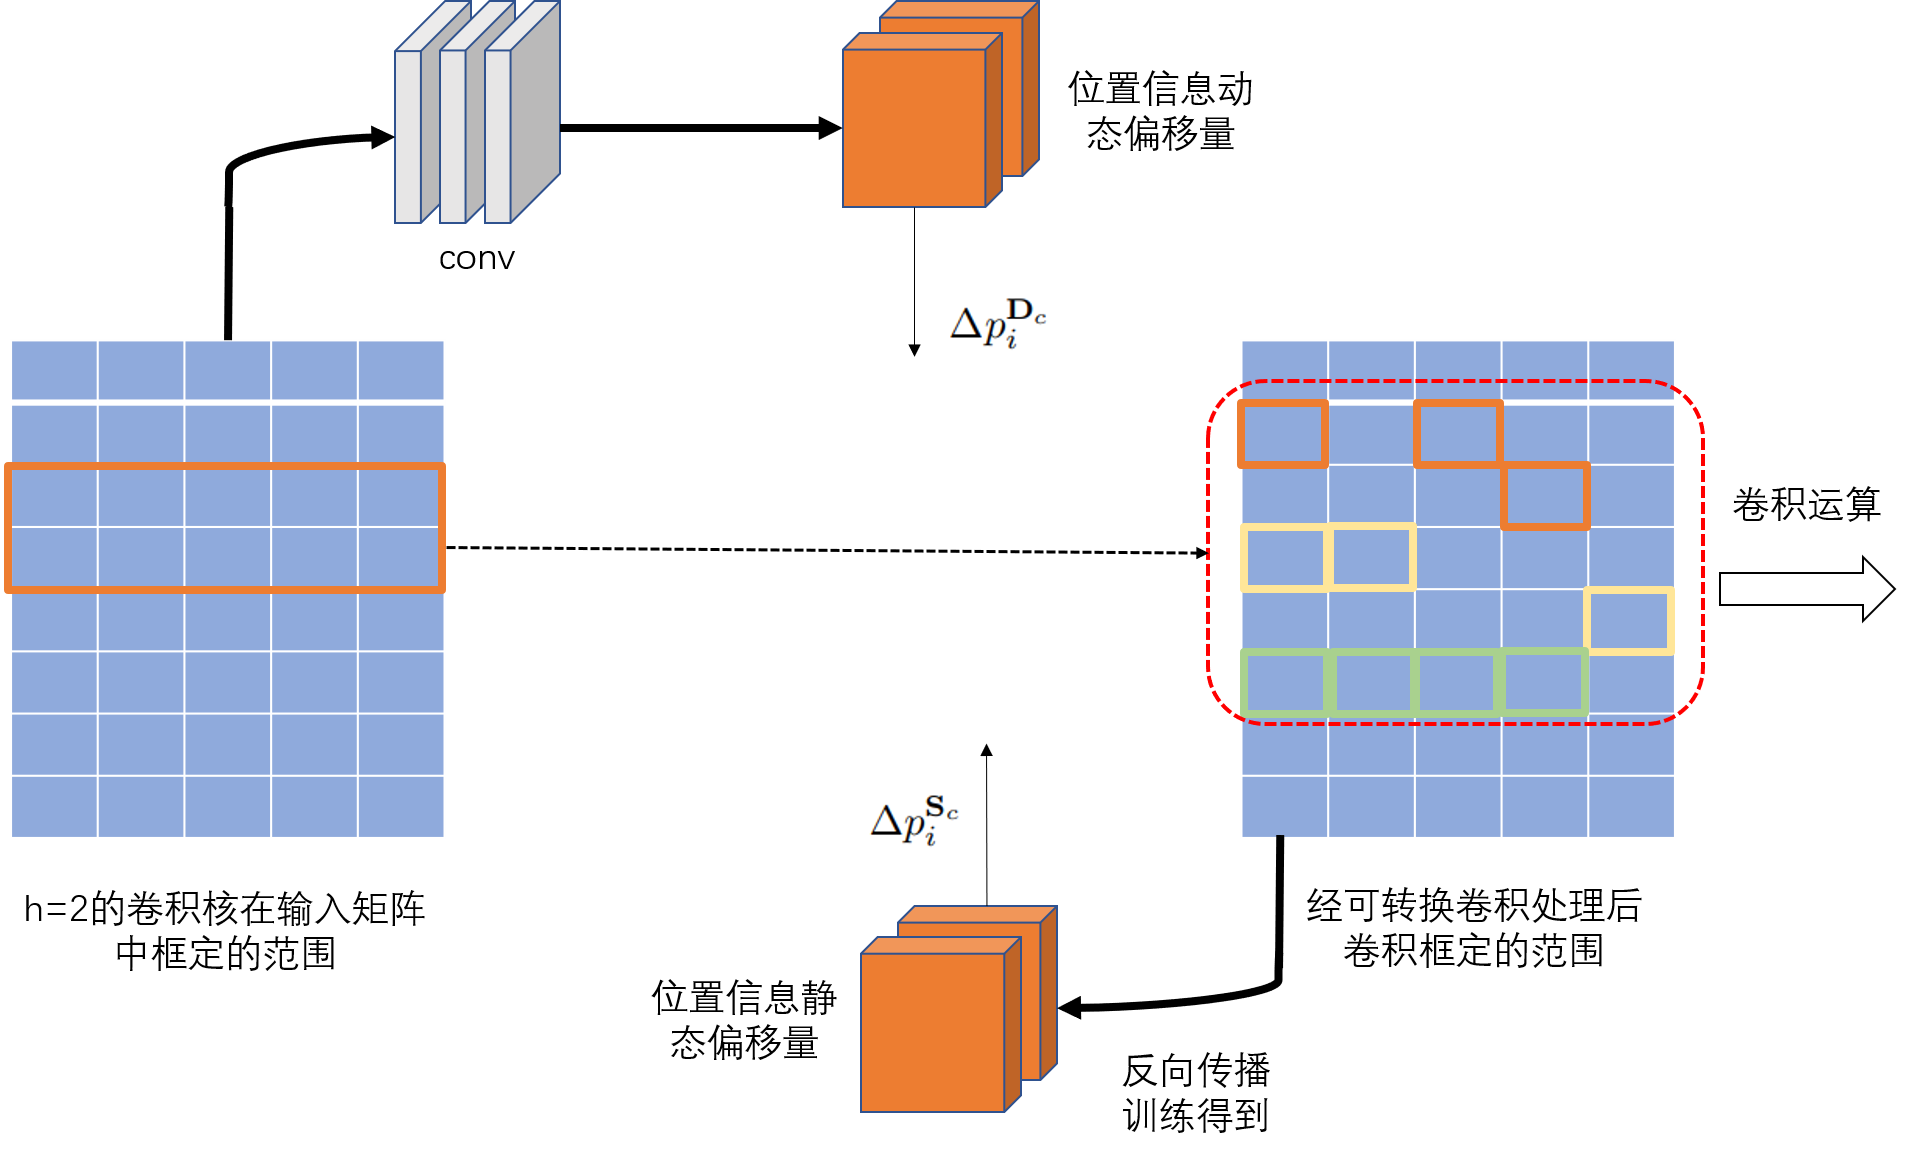
\includegraphics[scale=0.4]{./images/tansconv.jpg}
  \caption{接口分类模型中的transformable conv层}
  \label{fig:tansconv}
\end{figure}

3)输出层

由于卷积核卷积操作得到的结果是长条状,因此本文采用k-max pooling池化方法,k是超参数,经实验调整为4。
经过池化层处理后,得到4×64的特征矩阵作为lstm层的输入。
从64维的角度来看,每一维是一种高层语义特征的提取。
直观上,文本分类是顺序信息处理的过程。但是,从卷积神经网络以并行方式获得的特征序列不包含序列信息,LSTM专为顺序建模而设计,
可以进一步从CNN获得的特征序列中提取上下文信息。由于本模型层度较深参数较多,为防止训练时发生过拟合,
在lstm层后接入dropout(未在图中表示),最后利用softmax做分类决策。

实验结果表明,transformable cnn在测试集的表现要由于传统卷积层,这是由于它对变换特征的捕捉和建模能力得到了增强。
\section{引入字向量的BLSTM-ATT-CRF参数填充模型}
找到匹配的服务和相关的接口以后,在服务执行前需要从用户的输入语句提取出必要的执行参数,
因此本任务相较于分类任务更细粒度,对语义理解的要求更高,
这可以被看作命名实体识别问题,可以用序列标注算法提取执行参数。
对一个用户输入语句进行分词得到序列,如果分词操作出错,将丢失重要的语义信息,直接影响实体边界的预测,序列标注任务也不可能成功。
因此单纯依赖结巴分词工具分词以后获取输入序列信息使任务存在瓶颈,需要引入其他的embedding手段来降低分词错误带来的干扰,
我们选择在本模型中加入字符级的编码。
对于许多序列标记任务,访问过去(左)和将来(右)上下文都是有帮助的。但是,LSTM的隐藏状态$h_t$仅从过去获取信息,对右侧数据一无所知。 
双向LSTM(BLSTM)基本思想是将每个词向前和向后编码为两个单独的隐藏状态,以分别捕获过去和将来的信息,
然后将两个隐藏状态连接起来以形成最终输出,因此本模型特征提取部分主要依赖BLSTM。
同时我们选择条件随机场作为解码器,CRF考虑邻域标记之间的相关性,并针对给定输入语句联合解码得到最佳标记链。
综上所述,本节采用引入字向量的BLSTM-ATT-CRF模型\ref{fig:blstm-att-crf}解决参数填充问题,下面将详细介绍该模型:

\begin{figure}[htbp]
  \centering
  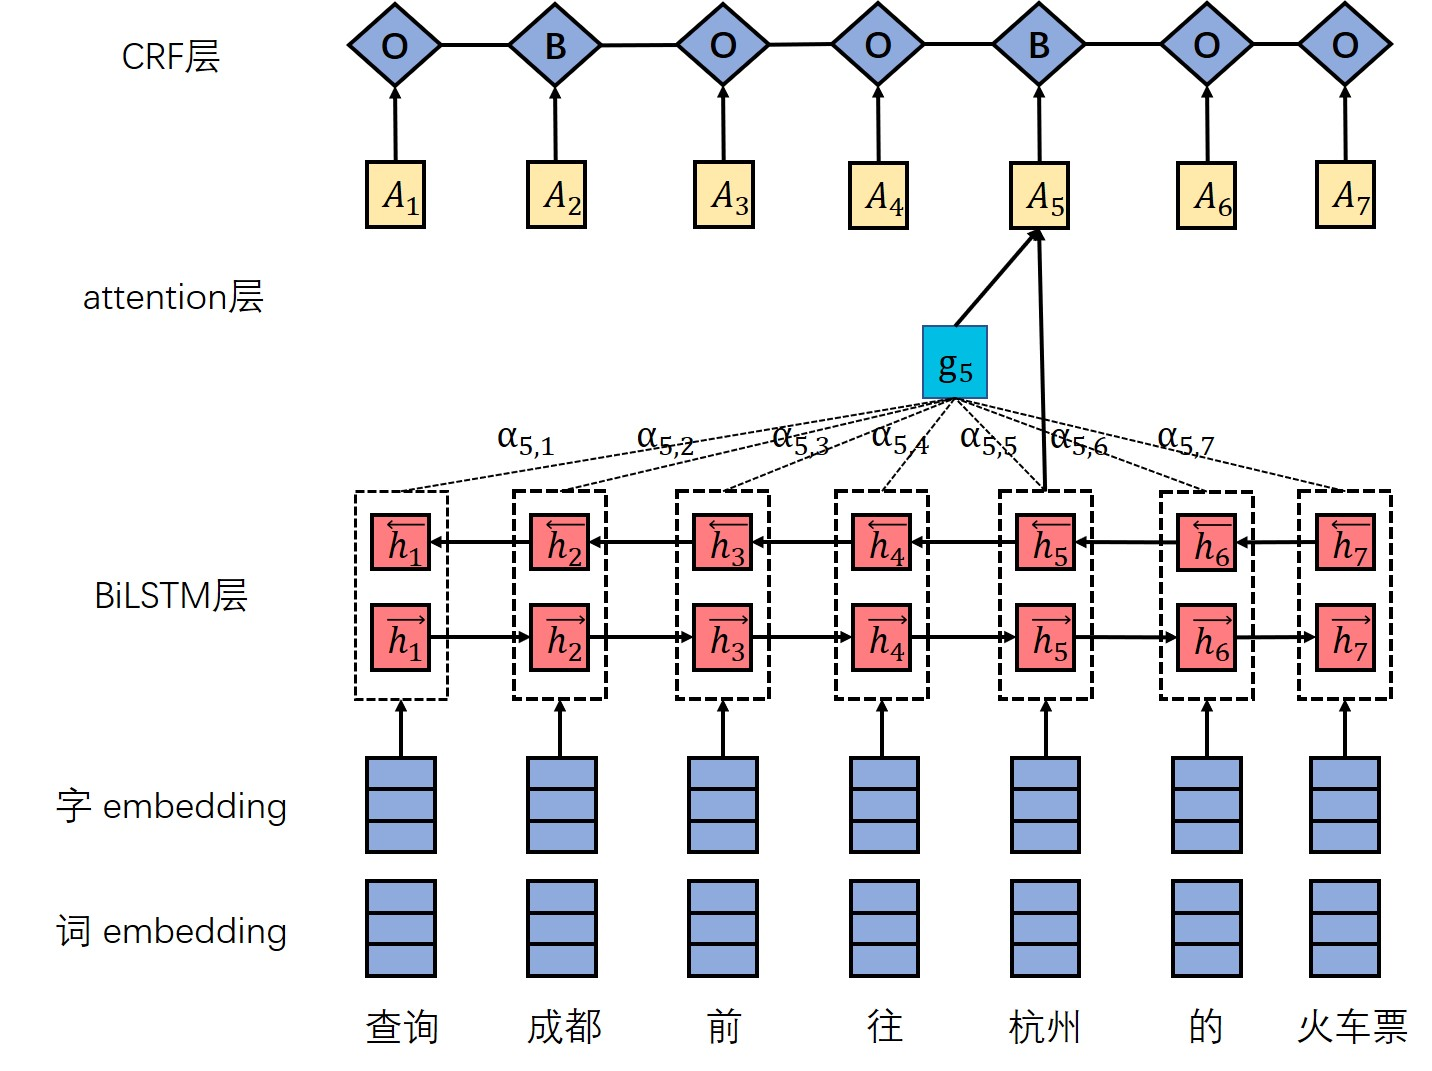
\includegraphics[scale=0.5]{./images/blstm-att-crf.jpg}
  \caption{参数填充模型}
  \label{fig:blstm-att-crf}
\end{figure}

1)输入层与embedding层

与前两个模型一致,首先,通过结巴分词工具得到词序列完成输入层的工作。但是,本模型除了词嵌入处理外,还引入了字符向量嵌入。设
$\mathbf{e}_{i}^{w}$表示用户输入语句词序列中第i个词的向量,$\mathbf{e}_{i}^{c}$指用户输入语句词序列中第i个词中所有字向量的表示,
则embedding层第i个词向BiLSTM层输入可表示为:
\begin{equation}
  \mathbf{x}_{i}=[\mathbf{e}_{i}^{w} ;\mathbf{e}_{i}^{c}]
\end{equation}
其中,我们会用另一个双向LSTM(图中未标出),输入为一句话的字向量序列,对于单词$w_i$的字向量$c_t(i,1),\dots,c_t(i,len(i))$(len(i)为词语的长度),
可以得到$\overrightarrow{\mathbf{h}}_{t(i, 1)}^{c}$,\dots,$\overrightarrow{\mathbf{h}}_{t(i, len(i))}^{c}$
和$\overleftarrow{\mathbf{h}}_{t(i, 1)}^{c}$,\dots,$\overleftarrow{\mathbf{h}}_{t(i, len(i))}^{c}$ ,上式中的$\mathbf{e}_{i}^{c}$由以下公式得出:
\begin{equation}
  \mathbf{e}_{i}^{c}=[\overrightarrow{\mathbf{h}}_{t(i, len(i))}^{c} ; \overleftarrow{\mathbf{h}}_{t(i, 1)}^{c}]
\end{equation}

2)BiLSTM-attention层

嵌入层的向量输入到双向LSTM网络中后,对每一个词$\mathbf{e}_{i}^{w}$,前向LSTM输出带有从左往右语义的向量$\overrightarrow{\mathbf{h}}_{i}$,
后向LSTM输出带有从右往左语义的向量$\overleftarrow{\mathbf{h}}_{i}$,我们将这两个向量拼接得到$\mathbf{h}_{i}=[\overrightarrow{\mathbf{h}}_{i} ;\overleftarrow{\mathbf{h}}_{i}]$
并对$\mathbf{h}_{i}$做self attention处理。
attention层主要运算工作是计算词与词之间的语义相似度,这里代表一个词$\mathbf{e}_{i}^{w}$的向量便是$\mathbf{h}_{i}$,则词i与词j之间的attention权重$α_{i,j}$可由下式得到:
\begin{equation}
\alpha_{t, j}=\frac{\exp \left(\operatorname{score}\left(\mathbf{h}_{i}, \mathbf{h}_{j}\right)\right)}{\sum_{k} \exp \left(\operatorname{score}\left(\mathbf{h}_{i}, \mathbf{x}_{k}\right)\right)}
\end{equation}
\begin{equation}
  \operatorname{score}(\mathbf{h}_{i}, \mathbf{h}_{j}))=\tanh \left(\mathbf{W}_{a}\left[\mathbf{h}_{i} ; \mathbf{h}_{j}\right]\right)
\end{equation}
attention权重由带有参数$\mathbf{W}_{a}$的感知器计算得到,以此来表示在理解当前词i时应该放多少注意力在词j上:
\begin{equation}
  \mathbf{g}_{i}=\sum_{j=1}^{N} \alpha_{i, j} \mathbf{h}_{j}
\end{equation}
于是我们得到了拥有全局视野的词i的向量表示$\mathbf{g}_{i}$,将它与$\mathbf{h}_{i}$拼接得到向量$\mathbf{a}_{i}=[\mathbf{g}_{i} ;\mathbf{h}_{i}]$作为CRF层的输入。

3)CRF层

在模型的最后,添加了CRF层以希望解码得到所有可能的标记路径中的最佳标记。 
t步长得到的标签预测向量可由$y_{t}^{s}=\operatorname{softmax}\left(W^{s} \overleftarrow{a}_{t}+b^{s}\right)$
得到,
引入标记转换矩阵$\mathbf{T}$,其中$T_{i,j}$表示上下连续两个单词中上一个被标记i以及下一个被标记j的转换分数,
而$T_{0,j}$表示标记j作为序列初始词标记的分数,该转换矩阵将做为模型的参数被训练。 
句子$\mathbf{X}$的被标记为$\mathbf{y}=(y_1,y_2,\dots,y_n)$的得分可由下式得出:
\begin{equation}
  s(\mathbf{X}, \mathbf{y})=\sum_{i=1}^{n}\left(T_{y_{i-1}, y_{i}}+P_{i, y_{i}}\right)
\end{equation}
$P_{i, y_{i}}$表示i位置softmax输出中标签$y_{i}$的概率,之后可以通过softmax函数推导出$\mathbf{X}$的被标记为$\mathbf{X}=(y_1,y_2,\dots,y_n)$的概率:
\begin{equation}
  p(\mathbf{y} \mid \mathbf{X})=\frac{e^{s(\mathbf{X}, \mathbf{y})}}{\sum_{\tilde{\mathbf{y}}} e^{s(\mathbf{X}, \tilde{\mathbf{y}})}}
\end{equation}
在训练时,模型的目标是使正确标注信息的概率最大。
设$y^{s}$表示槽的真实标签,$\hat y^{s}$表示槽的预测标签,插槽slot的损失函数采用max-margin(hinge loss):
\begin{equation}
\Delta\left(y^{s}, \hat{y}^{s}\right)=\sum_{t=1}^{T} 1\left\{y_{t}^{s} \neq \hat{y}_{t}^{s}\right\}
\end{equation}
对整个标签序列来说,损失函数定义如下:
\begin{equation}
L=\max (0, s(X,\hat{l}^{\hat{s}})+\Delta(y^{s}, \hat{y}^{\hat{s}})-s(X,y^{s}))
\end{equation}







\section{本章小结}

% \chapter{引入预训练模型的联合识别方法}

\section{算法描述}
研究表明,语言模型预训练对于学习通用的语言表示很有用。作为最新的语言模型预训练模型,BERT在许多语言理解任务中均取得了惊人的成绩,
BERT使用双向transformer网络结构来预训练语言模型,着眼于单词左右两侧的上下文,具有更强的表达能力,在大型语料库中训练得到的上下文敏感的语义向量
对语义消歧大有裨益,可以通过附加输出层对bert进行微调来完成模型构建。
在本章,针对跨界服务平台内部数据集有限的现状,我们希望利用bert预训练学到的语义编码能力,来提升第三章中提到的模型的准确率。

在跨界服务平台中,服务分类,接口分类和参数提取三者具有强相关的特性,对于系统内某一确定的服务,其接口和对应参数的全集也随之确定,
例如对于系统内部的天气服务,其接口仅有query类型,语义槽也是确定的city,date等,因此直觉上可见,可以显示利用任务之间的约束关系来提升模型的性能。
我们尝试了将三者loss函数叠加的隐式联合建模、服务与接口分类向参数提取提供信息流的单向联合识别以及服务分类、接口分类、参数填充三者联系显示建模
的交互式联合识别,以期寻求最优的解决方案,算法描述如表\ref{tab:suanfa2}。

\begin{table}[htb]
  \centering
  \caption{引入预训练模型的联合识别算法描述}
  \label{tab:suanfa2}
\begin{tabular}{p{150mm}}
\toprule
\textbf{算法1:}引入预训练模型的联合识别\\
\textbf{输入:} $L_0$=\{($S_i$,$y_i^d$,$y_i^i$,$y_i^s$)\},i $\in$ [1,n]\\
\textbf{输出:} $Model_{joint}$\\
\hline
\textbf{过程描述:}模型在训练时,输入的$S_i$为有用户意图的语句,直接将句子中每一个字按照
字向量输入进bert模型编码。模型参数初始化、批处理的数量
iterations = M 和每一批的样本数 batchsize、迭代次数 epoch = N 和当前迭代次数 i = 0\\
\textbf{while} i < N or 模型的性能达到终止条件 \textbf{do}\\
\qquad \qquad \textbf{for} j = 1,\dots ,M \textbf{do}\\
\qquad \qquad \qquad \qquad 随机抽取 batchsize 个训练集数据,前向传输在当前网络权值和输入下网络的输出\\
\qquad \qquad \qquad \qquad 反向传输调整模型参数,对bert参数fine-tuning\\
\qquad \qquad \textbf{end for}\\
\qquad \qquad 计算联合损失 Loss,更新梯度和模型的参数,对bert参数fine-tuning\\
\textbf{end while}\\
用训练好的联合识别模型对测试样本进行预测,计算准确率 Accuracy、损失 Loss\\
\bottomrule
\end{tabular}
\end{table}

\section{服务分类、接口分类与参数填充联合识别}
\subsection{slot-oriented联合识别}
如上小节所述,参数提取任务和服务分类、接口分类任务之间存在很强的关联性,而第三章的pipeline方法是三项任务各自独立,未能考虑到任务之间的关联性。
而建立联合损失函数的方法“隐式”考量了三个任务之间的联系,但并未明确为服务分类、
接口分类和服务参数填充之间进行显示的关联建模,考虑到由于服务参数填充通常高度依赖于前两个任务,
因此本节进行了单向联合识别的尝试,提出了单向联合模型,以期通过整合全局信息流方向来优化获得更好的语义理解结果。
同时,和上一章一样,注意力机制被引入到模型中,在编码时提供精确的关注焦点。
本节的模型着重于介绍如何通过引入参数提取门控机制来对服务分类,接口分类和服务参数填充之间进行显式关系建模。

\begin{figure}[htbp]
    \centering
    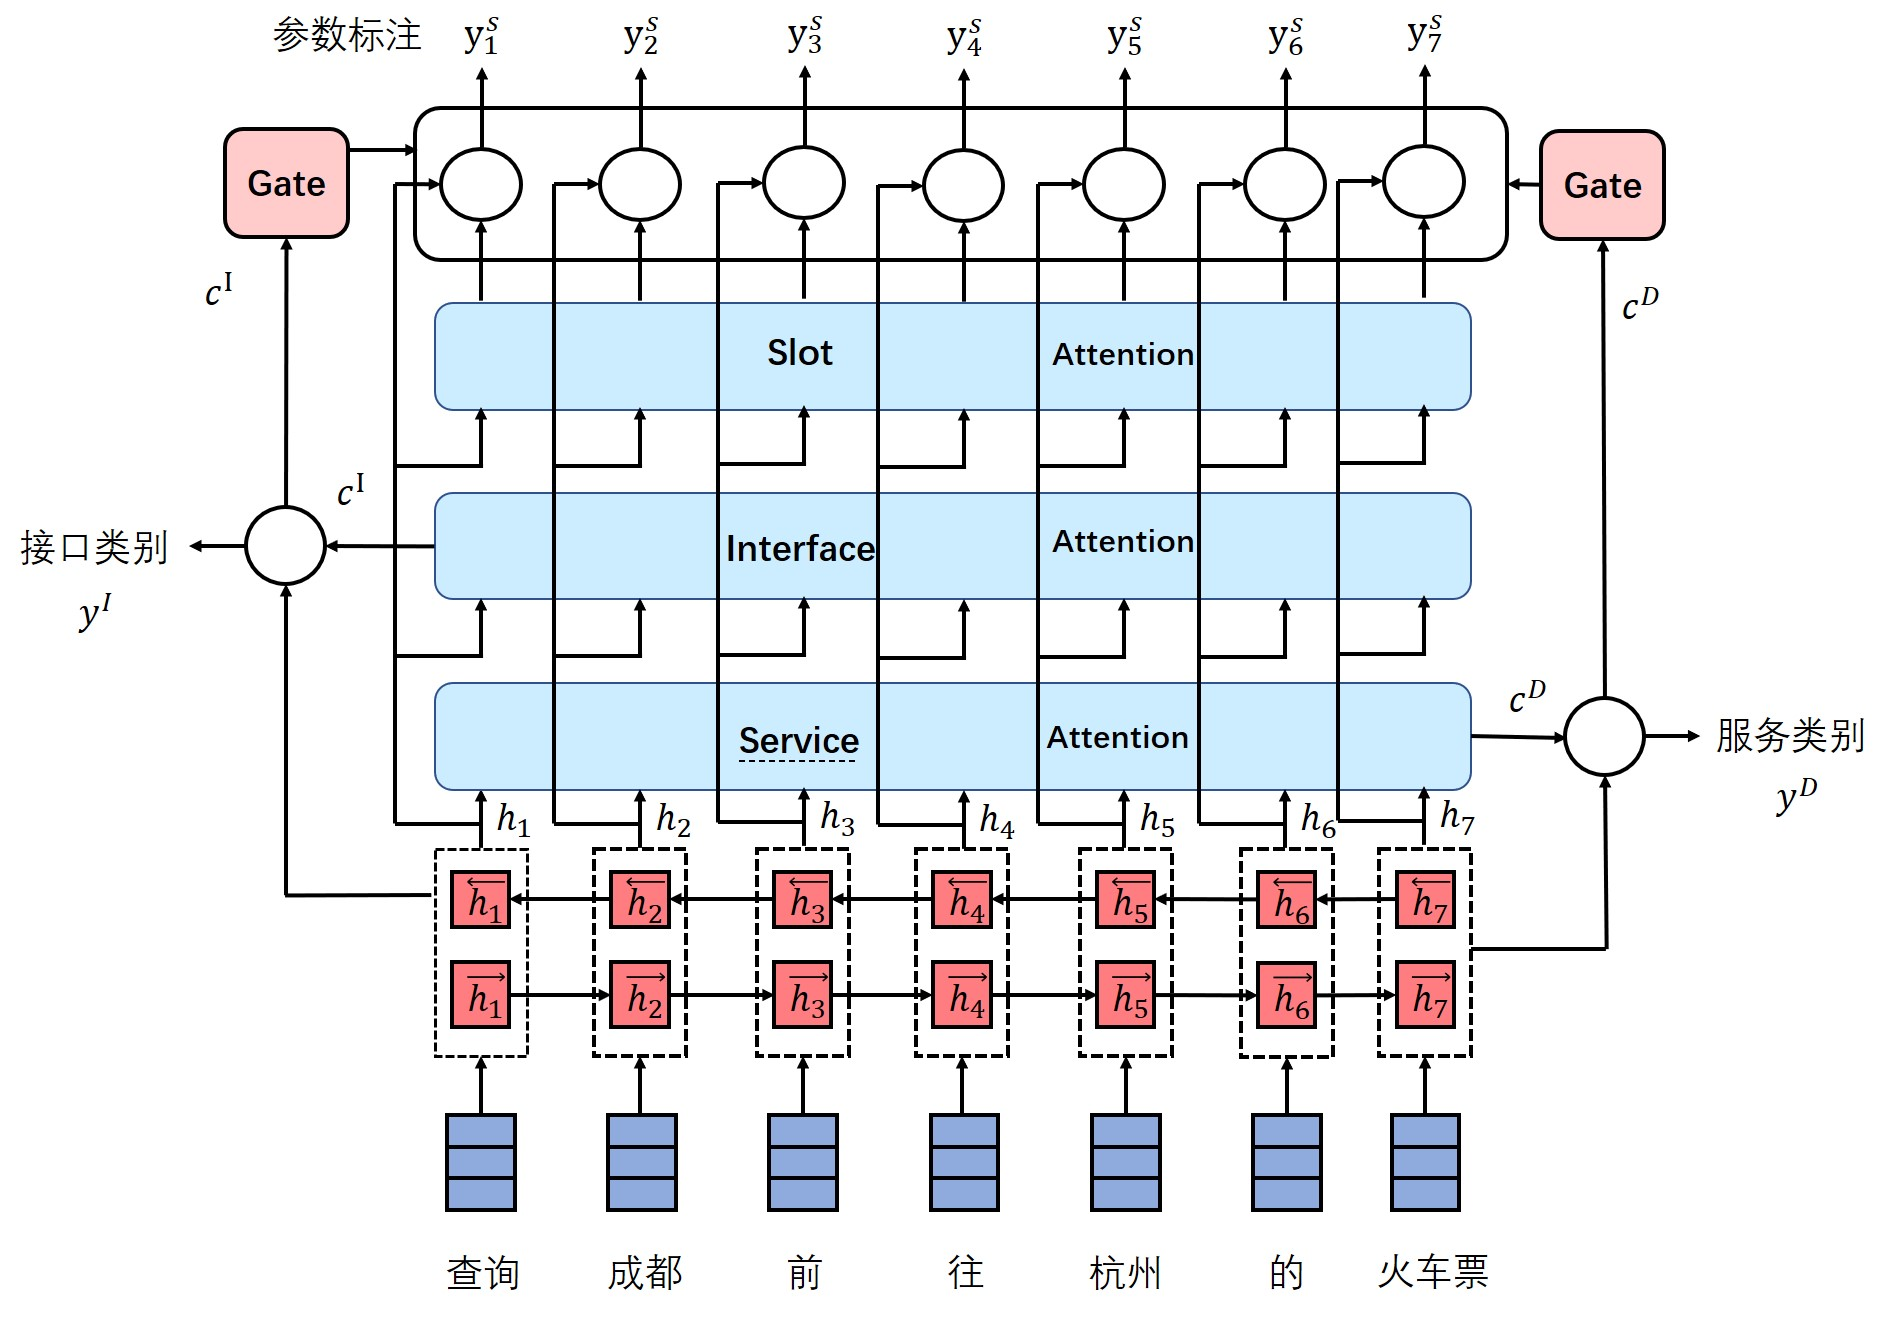
\includegraphics[width=17cm]{./images/lianhe.jpg}
    \caption{slot-oriented联合识别模型}
    \label{fig:lianhe1}
  \end{figure}

如图\ref{fig:lianhe}所示,设slot-oriented联合识别模型输入的词序列是x=[$x_{1}$,$x_{2}$,\dots,$x_{T}$],$x_{i}$经过双向LSTM处理后
得到的结果是$\overleftarrow{\mathbf{h}}_{i}$和$\overrightarrow{\mathbf{h}}_{i}$,
拼接以后在第i步得到的结果是$\mathbf{h}_{i}=[\overrightarrow{\mathbf{h}}_{i} ;\overleftarrow{\mathbf{h}}_{i}]$。

(1)attention层

我们在联合模型中共设置了三层注意力机制,分别用于服务分类、接口分类与参数填充,三者的attention原理相同,只是会训练各自的参数,因此可以合并介绍。
设BLSTM得到的隐层向量序列为$h_{1}$,$h_{2}$,\dots,$h_{T}$,我们引入上下文向量${c}_{i}$来表示经过attention权重$α_{i,j}$和处理后的BLSTM隐层向量,
具体的${c}_{i}^{D}$,${c}_{i}^{I}$,${c}_{i}^{S}$分别表示用于服务分类、接口分类与参数填充任务的上下文向量:
\begin{equation}
    \mathbf{c}_{i}=\sum_{j=1}^{T} \alpha_{i, j} \mathbf{h}_{j}
  \end{equation}
  其中$\alpha_{i, j}$也根据所在具体的attention层不同分为$\alpha_{i, j}^{D}$,$\alpha_{i, j}^{I}$,$\alpha_{i, j}^{S}$,计算公式如下:
  \begin{equation}
    \alpha_{t, j}=\frac{\exp \left(\operatorname{score}\left(\mathbf{h}_{i}, \mathbf{h}_{j}\right)\right)}{\sum_{k} \exp \left(\operatorname{score}\left(\mathbf{h}_{i}, \mathbf{x}_{k}\right)\right)}
    \end{equation}
    \begin{equation}
      \operatorname{score}(\mathbf{h}_{i}, \mathbf{h}_{j}))=\tanh \left(\mathbf{W}\left[\mathbf{h}_{i} ; \mathbf{h}_{j}\right]\right)
    \end{equation}
显然这里的$\mathbf{W}$可根据任务具体分为$\mathbf{W}_D$,$\mathbf{W}_I$,$\mathbf{W}_S$

(2)服务分类

我们以(1)中计算服务分类上下文向量的方法可以得到${c}_{i}^{D}$,再从BLSTM中取$\overleftarrow{\mathbf{h}}_{1}$和$\overrightarrow{\mathbf{h}}_{T}$,
$c^{D}$表示所有步骤得到的$c_i^{D}$的均值,服务的类别预测可由下式得到:
\begin{equation}
    y^{D}=\operatorname{softmax}\left(W^{D}\left(\overleftarrow{\mathbf{h}}_{1}+\overrightarrow{\mathbf{h}}_{T}+c^{D}\right)\right)
  \end{equation}
  \begin{equation}
    c^{D}=\frac{1}{T}\sum_{i=1}^{T} c_i^{D}
  \end{equation}

(3)接口分类

  我们以(1)中计算接口分类上下文向量的方法可以得到${c}_{i}^{D}$,再从BLSTM中取$\overleftarrow{\mathbf{h}}_{1}$和$\overrightarrow{\mathbf{h}}_{T}$,
  $c^{I}$表示所有步骤得到的$c_i^{I}$的均值,接口的类别预测可由下式得到:
  \begin{equation}
      y^{I}=\operatorname{softmax}\left(W^{I}\left(\overleftarrow{\mathbf{h}}_{1}+\overrightarrow{\mathbf{h}}_{T}+c^{I}\right)\right)
    \end{equation} 
    \begin{equation}
        c^{I}=\frac{1}{T}\sum_{i=1}^{T} c_i^{I}
      \end{equation}

      \begin{figure}[htbp]
        \centering
        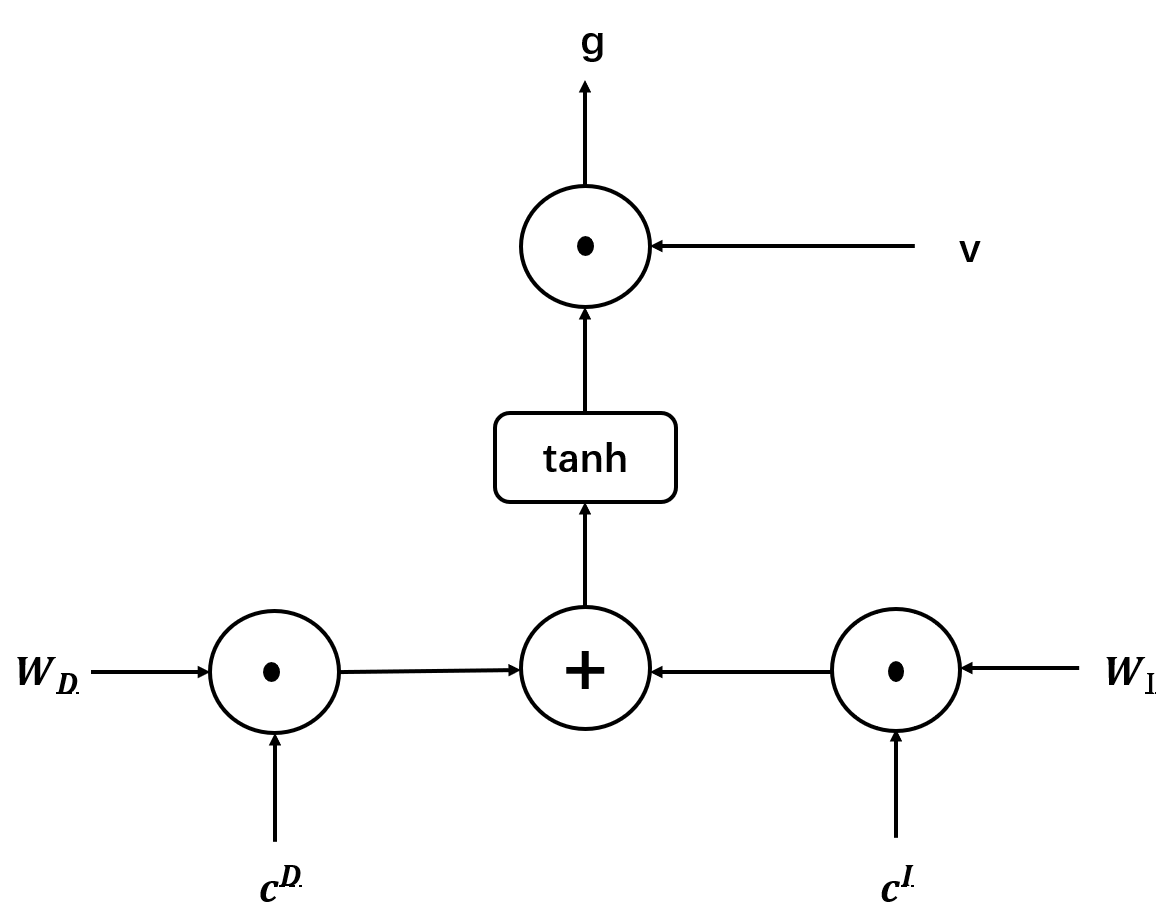
\includegraphics[scale=0.3]{./images/gate.jpg}
        \caption{gate结构}
        \label{fig:gate}
      \end{figure}

(4)参数提取

如图\ref{fig:gate}中的gate,我们引入参数提取的控制门利用服务类型上下文向量${c}_{i}^{D}$和接口类型上下文向量${c}_{i}^{I}$来建模服务、接口与参数填充的关系
以期提高参数提取的准确率。${c}^{D}$,${c}^{I}$,${c}_{i}^{S}$会在每一个步长传入gate结构中计算:
\begin{equation}
    g=\sum v \cdot \tanh (c_{i}^{S}+W_D \cdot c^{D}+W_I \cdot c^{I})
  \end{equation}
其中$\mathbf{v},\mathbf{W}_D,\mathbf{W}_I$是可训练的参数,数值g可以被看作联合上下文向量${c}^{D}$,${c}^{I}$,${c}_{i}^{S}$计算得到的权值,
较大的g表示slot上下文向量和D、I上下文向量“注意力一致”,可以推断出该语义槽和服务、接口之间的相关性更强,该词更有可能是我们需要提取的参数。
最终第i个词的标签类别信息可由下式计算得出:
\begin{equation}
    y_{i}^{S}=\operatorname{softmax}\left(W_{h y}^{S}\left(h_{i}+c_{i}^{S} \cdot g\right)\right)
  \end{equation}

(5)联合目标函数

为了同时完成服务分类、接口分类与参数填充三项任务,需要建立联合损失函数,假设$y^D,y^I,y^S$表示正确的类别与标注,我们的目标
便是使在输入为$\mathbf{x}$的条件下概率$p\left(y^{S}, y^{I},y^{D} \mid \mathbf{x}\right)$最大:
\begin{equation}
    \begin{array}{l}
        p\left(y^{S}, y^{I},y^{D} \mid \mathbf{x}\right) \\
        =p\left(y^{D} \mid \mathbf{x}\right) p\left(y^{I} \mid \mathbf{x}\right) \prod_{t=1}^{T} p\left(y_{t}^{S} \mid \mathbf{x}\right) \\
        =p(y^{D} \mid x_{1}, \ldots, x_{T}) p(y^{I} \mid x_{1}, \ldots, x_{T}) \prod_{t=1}^{T} p(y_{t}^{S} \mid x_{1}, \ldots, x_{T})
        \end{array}
    \end{equation}

\subsection{co-interactive联合识别}
上一个的模型完成了从各任务独自建模到服务分类、接口分类向参数填充传递信息流的转换,
但只考虑了从服务和接口到参数填充的单向信息流,而忽略了显式应用参数填充(语义槽)信息来指导前两项任务,这导致无法有效地建立双向连接。
直观的讲,如果用户的意图是调用平台内部的火车票查询服务,他输入的语句更可能出现诸如起始终点城市,日期等语义槽;反之,如果一句话中包含了
出发的起始,目的地和日期,那用户的意图更可能是调用行程相关的服务。因此,考虑任务与任务之间的交互影响十分重要\ref{fig:lianhe2}。

在本模型中,核心组件是协同交互层模块,用于对任务与任务之间关系的显示建模,旨在考虑任务与任务的交叉影响以及相互促进。
具体来说,在协同交互层模块中,
我们首先在服务、接口和参数填充分别应用注意力机制,以捕获初始的显式向量表示,从而提取三个任务的语义信息。
其次,将明确的服务、接口和参数填充表示形式馈入一个共同交互的注意层,以进行信息流的多向充分融合。
将服务分类向量视为查询$Q_D$,参数填充向量视为键$K_S$以及值$K_S$,以获取可感知服务分类信息的参数填充向量表示信息并反馈给服务分类任务;
接口分类向量视为键$K_I$以及值$K_I$,以获取可感知服务分类信息的接口向量表示信息并反馈给服务分类任务。
将接口分类向量视为查询$Q_I$,参数填充向量视为键$K_S$以及值$K_S$,以获取可感知接口分类信息的参数填充向量表示信息并反馈给接口分类任务;
服务分类向量视为键$K_D$以及值$K_D$,以获取可感知接口分类信息的服务向量表示信息并反馈给接口分类任务。
将参数填充向量视为查询$Q_S$,服务分类向量视为键$K_D$以及值$K_D$,以获取可感知参数填充信息的服务分类向量表示信息并反馈给参数填充任务;
接口分类向量视为键$K_I$以及值$K_I$,以获取可感知参数填充信息的接口向量表示信息并反馈给参数填充任务。
基于此操作,可以建立多个任务之间的显示连接,背后的原理是通过协同互动的注意力机制获取相应的交互信息。
参考transformer的设计,可以将协同交互模块堆叠在一起以形成一个层次结构,该层次结构使任务之间能够进行多次交互,从而实现增量捕获交互信息来达到彼此丰富。

\begin{figure}[htbp]
  \centering
  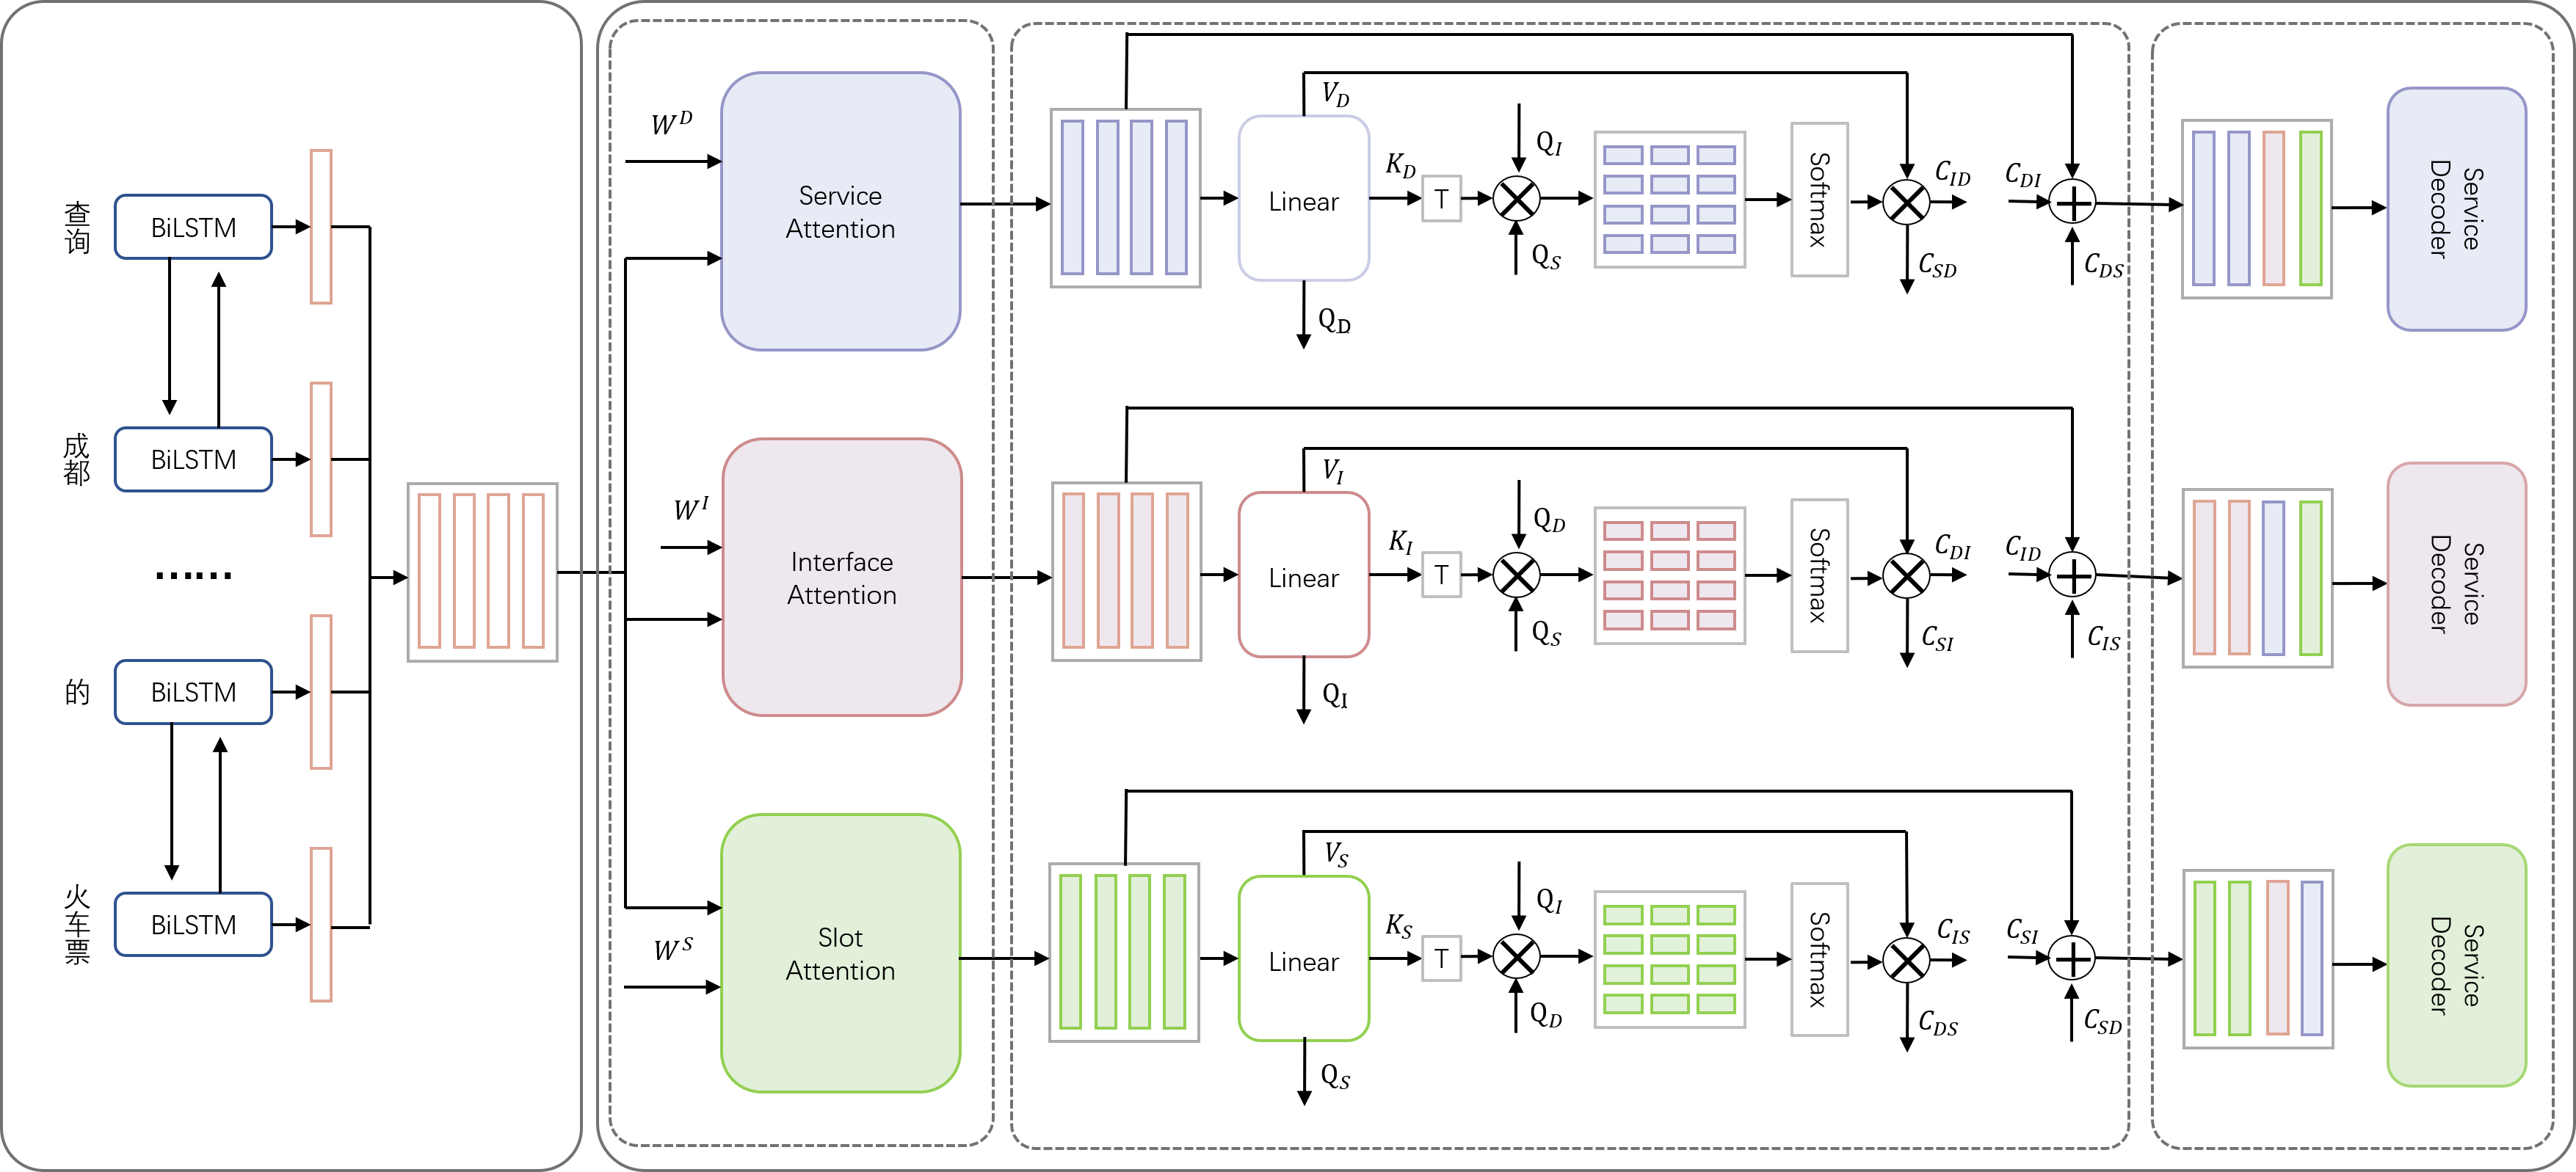
\includegraphics[width=16cm]{./images/co-interactive.jpg}
  \caption{交互式联合识别模型}
  \label{fig:lianhe2}
\end{figure}


交互式联合识别模型的结构如图\ref{fig:lianhe2}所示,主要包含的部分是:共享编码层,注意力层,协同交互层,独立解码层,接下将分别介绍:

(1)共享编码层

我们使用双向LSTM作为编码器,设输入词序列是x=[$x_{1}$,$x_{2}$,\dots,$x_{n}$](n为词的数量),$x_{i}$经过双向LSTM处理后
得到的结果是$\overleftarrow{\mathbf{h}}_{i}$和$\overrightarrow{\mathbf{h}}_{i}$,拼接以后在第i步得到的结果是$\mathbf{h}_{i}=[\overrightarrow{\mathbf{h}}_{i} ;\overleftarrow{\mathbf{h}}_{i}]$,
因此编码后得到的矩阵为$\mathbf{H}$=[$h_{1}$,$h_{2}$,\dots,$h_{n}$]。

(2)自注意力层

我们为服务分类、接口分类和参数填充三个任务分别引入了自注意力机制,将自注意力层处理以后得到的向量作为相应任务的矩阵表示传入协同交互层。
三者的attention原理相同,只是会训练各自的参数,因此可以合并介绍。
我们引入上下文向量${c}_{i}$来表示经过attention权重$α_{i,j}$处理后的BLSTM隐层向量:
\begin{equation}
    \mathbf{c}_{i}=\sum_{j=1}^{n} \alpha_{i, j} \mathbf{h}_{j}
  \end{equation}
  经过attention处理的句子矩阵表示为$\mathbf{C}$=[$c_{1}$,$c_{2}$,\dots,$c_{n}$],其中$\alpha_{i, j}$根据所在具体的attention层不同分为$\alpha_{i, j}^{D}$,$\alpha_{i, j}^{I}$,$\alpha_{i, j}^{S}$,计算公式如下:
  \begin{equation}
    \alpha_{t, j}=\frac{\exp \left(\operatorname{score}\left(\mathbf{h}_{i}, \mathbf{h}_{j}\right)\right)}{\sum_{k} \exp \left(\operatorname{score}\left(\mathbf{h}_{i}, \mathbf{x}_{k}\right)\right)}
    \end{equation}
    \begin{equation}
      \operatorname{score}(\mathbf{h}_{i}, \mathbf{h}_{j}))=\tanh \left(\mathbf{W}\left[\mathbf{h}_{i} ; \mathbf{h}_{j}\right]\right)
    \end{equation}
显然这里的$\mathbf{W}$根据任务不同分为$\mathbf{W}_D$,$\mathbf{W}_I$,$\mathbf{W}_S$,最后我们将H矩阵与attention处理的C矩阵相加:
\begin{equation}
  \mathbf{H}=\mathbf{H}+\mathbf{C}
\end{equation}
这里H根据训练时参数的不同分为三类$\mathbf{H}_{D},\mathbf{H}_{I},\mathbf{H}_{S}$,分别表示服务分类、接口分类向参数填充三项任务语义相关的显示的矩阵表示。

(3)协同交互层

本层是多个任务的信息流建立信息交换的核心层,上层共得到三个矩阵$\mathbf{H}_{D},\mathbf{H}_{I},\mathbf{H}_{S}$,他们是任务相关的独立的语义表示,本层主要目的
是在借助其他两项任务指导下更新当前任务对应的H矩阵,达到交互信息流的目的,提高模型准确率。
首先我们将$\mathbf{H}_{D},\mathbf{H}_{I},\mathbf{H}_{S}$分别做三组线性变换得到矩阵($\mathbf{Q}_{D},\mathbf{Q}_{I},\mathbf{Q}_{S}$),
($\mathbf{K}_{D},\mathbf{K}_{I},\mathbf{K}_{S}$),($\mathbf{V}_{D},\mathbf{V}_{I},\mathbf{V}_{S}$),之后的计算借鉴attention思想。
对于服务分类任务,将$\mathbf{Q}_{D}$做为queries,$\mathbf{K}_{I}$做为keys和$\mathbf{V}_{I}$做为values,$\mathbf{K}_{S}$做为keys和$\mathbf{V}_{S}$做为values,做以下处理来达到信息的交互:
\begin{equation}
  \mathbf{C}_{\mathbf{DI}}=\operatorname{softmax}\left(\frac{\mathbf{Q}_{\mathbf{D}} \mathbf{K}_{\mathbf{I}}^{\top}}{\sqrt{d_{k}}}\right) \mathbf{V}_{\mathbf{I}}\\
\end{equation}
\begin{equation}  
\mathbf{C}_{\mathbf{DS}}=\operatorname{softmax}\left(\frac{\mathbf{Q}_{\mathbf{D}} \mathbf{K}_{\mathbf{S}}^{\top}}{\sqrt{d_{k}}}\right) \mathbf{V}_{\mathbf{S}}\\
\end{equation}
\begin{equation}  
\mathbf{H}_\mathbf{D}=\mathbf{H}_\mathbf{D}+\mathbf{C}_{\mathbf{DI}}+\mathbf{C}_{\mathbf{DS}}
\end{equation}
对于接口分类任务,将$\mathbf{Q}_{I}$做为queries,$\mathbf{K}_{D}$做为keys和$\mathbf{V}_{D}$做为values,$\mathbf{K}_{S}$做为keys和$\mathbf{V}_{S}$做为values,做以下处理来达到信息的交互:
\begin{equation}
  \mathbf{C}_{\mathbf{ID}}=\operatorname{softmax}\left(\frac{\mathbf{Q}_{\mathbf{I}} \mathbf{K}_{\mathbf{D}}^{\top}}{\sqrt{d_{k}}}\right) \mathbf{V}_{\mathbf{D}}\\
\end{equation}
\begin{equation}
  \mathbf{C}_{\mathbf{IS}}=\operatorname{softmax}\left(\frac{\mathbf{Q}_{\mathbf{I}} \mathbf{K}_{\mathbf{S}}^{\top}}{\sqrt{d_{k}}}\right) \mathbf{V}_{\mathbf{S}}\\
\end{equation}
\begin{equation}
  \mathbf{H}_\mathbf{I}=\mathbf{H}_\mathbf{I}+\mathbf{C}_{\mathbf{ID}}+\mathbf{C}_{\mathbf{IS}}
\end{equation}
对于接口分类任务,将$\mathbf{Q}_{S}$做为queries,$\mathbf{K}_{D}$做为keys和$\mathbf{V}_{D}$做为values,$\mathbf{K}_{I}$做为keys和$\mathbf{V}_{I}$做为values,做以下处理来达到信息的交互:
\begin{equation}
  \mathbf{C}_{\mathbf{SD}}=\operatorname{softmax}\left(\frac{\mathbf{Q}_{\mathbf{S}} \mathbf{K}_{\mathbf{D}}^{\top}}{\sqrt{d_{k}}}\right) \mathbf{V}_{\mathbf{D}}\\
\end{equation}
\begin{equation}
  \mathbf{C}_{\mathbf{SI}}=\operatorname{softmax}\left(\frac{\mathbf{Q}_{\mathbf{S}} \mathbf{K}_{\mathbf{I}}^{\top}}{\sqrt{d_{k}}}\right) \mathbf{V}_{\mathbf{I}}\\
\end{equation}
\begin{equation}
  \mathbf{H}_\mathbf{S}=\mathbf{H}_\mathbf{S}+\mathbf{C}_{\mathbf{SD}}+\mathbf{C}_{\mathbf{SI}}
\end{equation}

其中$d_k$是Q,K矩阵的列数。我们认为经过上面计算更新过后的矩阵$\mathbf{H}_{D},\mathbf{H}_{I},\mathbf{H}_{S}$,包含了更丰富的语义信息,
实现了多任务之间信息的交互。
同时如图中标识(N×),N为超参数,协同交互层可堆叠在一起形成层次结构,使任务之间能够进行多次交互,实现增量捕获交互信息来达到彼此丰富。

(4)独立解码层

在经过共享的协同交互层以后,各任务拥有自己独立的解码层。
对于服务分类任务,我们使用上一章介绍的CNN的max-pooling方法,将$\mathbf{H}_{D}$经过max-pooling处理得到一个句子语义级表示的向量$\mathbf{M}_D$,
之后经过softmax函数:
\begin{equation}
  \mathbf{y}^{D}=\operatorname{softmax} (\mathbf{W}^{D}\mathbf{M}_D+\mathbf{b}^{D})
\end{equation}
\begin{equation}
  \mathbf{O}^{D}=\operatorname{argmax} (\mathbf{y}^{D})
\end{equation}
$\mathbf{y}^{D}$是输出的服务类别的分布,$\mathbf{O}^{D}$是预测的服务类别,$\mathbf{W}^{D}$和$\mathbf{b}^{D}$都是训练的参数。
对于接口分类任务解码器也做同样的处理,使用CNN的max-pooling方法,将$\mathbf{H}_{D}$经过max-pooling处理得到一个句子语义级表示的向量$\mathbf{M}_I$,
之后经过softmax函数:
\begin{equation}
  \mathbf{y}^{I}=\operatorname{softmax} (\mathbf{W}^{I}\mathbf{M}_I+\mathbf{b}^{I})
\end{equation}
\begin{equation}
  \mathbf{O}^{I}=\operatorname{argmax} (\mathbf{y}^{I})
\end{equation}
$\mathbf{y}^{I}$是输出的服务类别的分布,$\mathbf{O}^{I}$是预测的服务类别,$\mathbf{W}^{I}$和$\mathbf{b}^{I}$都是训练的参数。
对于参数提取即语义槽填充任务,为了更好的建模标签与标签之间的依赖性,我们在解码层加了CRF处理,如下式所示:
\begin{equation}
  \mathbf{O}_{\mathbf{S}} =\mathbf{W}^{\mathbf{S}} {\mathbf{H}}_{\mathbf{S}}+\mathbf{b}_{\mathbf{S}} 
\end{equation}
\begin{equation}
  P\left(\hat{\mathbf{y}} \mid \mathbf{O}_{\mathbf{S}}\right) =\frac{\sum_{i=1} \exp f\left(y_{i-1}, y_{i}, \mathbf{O}_{\mathbf{S}}\right)}{\sum_{y^{\prime}} \sum_{i=1} \exp f\left(y_{i-1}^{\prime}, y_{i}^{\prime}, \mathbf{O}_{\mathbf{S}}\right)}
  \end{equation}
  $f(y_{i-1}, y_{i}, \mathbf{O}_{\mathbf{S}})$表示从标签$y_{i-1}$到标签$y_{i}$的转移分数,以及标签$y_{i}$自身的得分。
同时我们采用联合损失函数的形式对三项任务一起训练,服务分类预测的交叉熵损失函数可记为:
\begin{equation}
\mathcal{L}_{1} \triangleq-\sum_{j=1}^{m} \hat{\mathbf{y}}^{j, \mathbf{D}} \log \left(\mathbf{y}^{j, \mathbf{D}}\right)
\end{equation}
同理,接口分类交叉熵损失函数可记为:
\begin{equation}
  \mathcal{L}_{2} \triangleq-\sum_{j=1}^{m} \hat{\mathbf{y}}^{j, \mathbf{I}} \log \left(\mathbf{y}^{j, \mathbf{I}}\right)
  \end{equation}
  参数语义槽填充交叉熵损失函数可记为:
  \begin{equation}
    \mathcal{L}_{3} \triangleq-\sum_{j=1}^{m} \sum_{i=1}^{n_{j}} \hat{\mathbf{y}}_{i}^{j, \mathbf{S}} \log \left(\mathbf{y}_{i}^{j, \mathbf{S}}\right)
  \end{equation}
  其中$\hat{\mathbf{y}}^{j, \mathbf{D}},\hat{\mathbf{y}}^{j, \mathbf{I}},\hat{\mathbf{y}}_{i}^{j, \mathbf{S}}$为真实值,m是训练的数据总量,联合损失函数
  可表示为:
  \begin{equation}
    \mathcal{L}_{\theta}=\alpha \mathcal{L}_{1}+\beta \mathcal{L}_{2}+(1-\alpha-\beta) \mathcal{L}_{3}
  \end{equation}
  其中$\alpha,\beta$为超参数。

\section{结合bert的模型}

大量研究表明,语言模型预训练对于学习通用语言表示很有用,作为最新的语言模型预训练模型,BERT在许多语言理解任务中均取得了惊人的成绩。
bert预训练模型的使用可以避免从头开始训练新模型,它通过利用大量非标注数据来学习语言的通用表示形式。

官方提供了不同参数的多版本bert供用户使用,本文从中选择的是BERT-Base Chinese,
其中核心参数 L = 12, H = 768, A = 12 ,params的总量为 110 M。具体来说, L = 12 指 Transformer 的层数为 12 层,
 H = 768 表示 Transformer 内部 包含 768 个隐含单元, A = 12 表示多头自制力机制中自注意力机制个数为 12 个\cite{devlin2018bert}。
 BERT依赖于Transformer,一个基本的Transformer由一个读取文本输入的编码器和一个对任务进行预测的解码器组成。
BERT编码器的输入是一系列token,这些token首先被转换为矢量,然后在神经网络中进行处理。
但是在开始处理之前,BERT需要对输入进行处理并用一些额外的元数据修饰:

1.令牌嵌入:在第一个句子的开头将[CLS]令牌添加到输入的单词令牌中,并在每个句子的末尾插入[SEP]令牌。

2.段嵌入:将指示输入属于句子A或句子B的标记添加到每个标记,这使编码器能够区分输入属于哪个句子。

3.位置嵌入:将位置嵌入添加到每个标记,以指示词在句子中的位置。

因此,引入bert模型以后我们不再需要结巴分词工具,直接将句子按字向量序列输入bert模型编码,bert对输入的处理如图\ref{fig:bertInput}。
\begin{figure}[htbp]
  \centering
  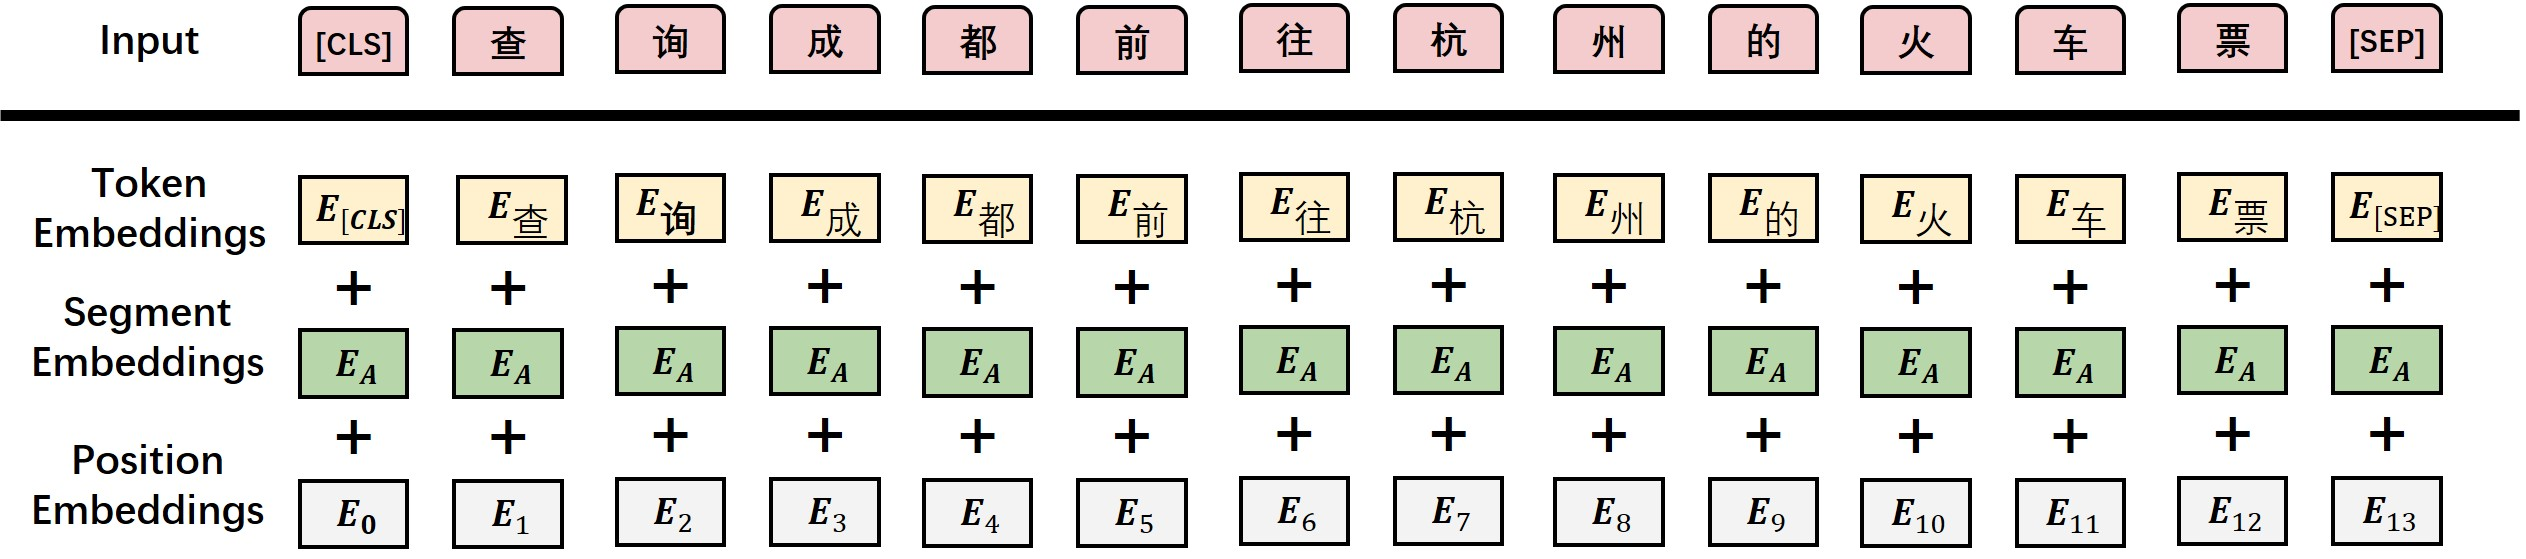
\includegraphics[width=18cm]{./images/bertInput.jpg}
  \caption{bert对输入的处理}
  \label{fig:bertInput}
\end{figure}

\subsection{bert-base联合识别模型}
首先,我们提出最简版的bert-base模型,
将服务分类、接口分类和参数填充三个任务利用联合损失函数隐式的建模,本模型主要起对照组的作用,
来验证引入bert是否能够给NLU带来增益,同时可以作为下一个模型的baseline,模型架构如图\ref{fig:bert-base}所示。

\begin{figure}[htbp]
  \centering
  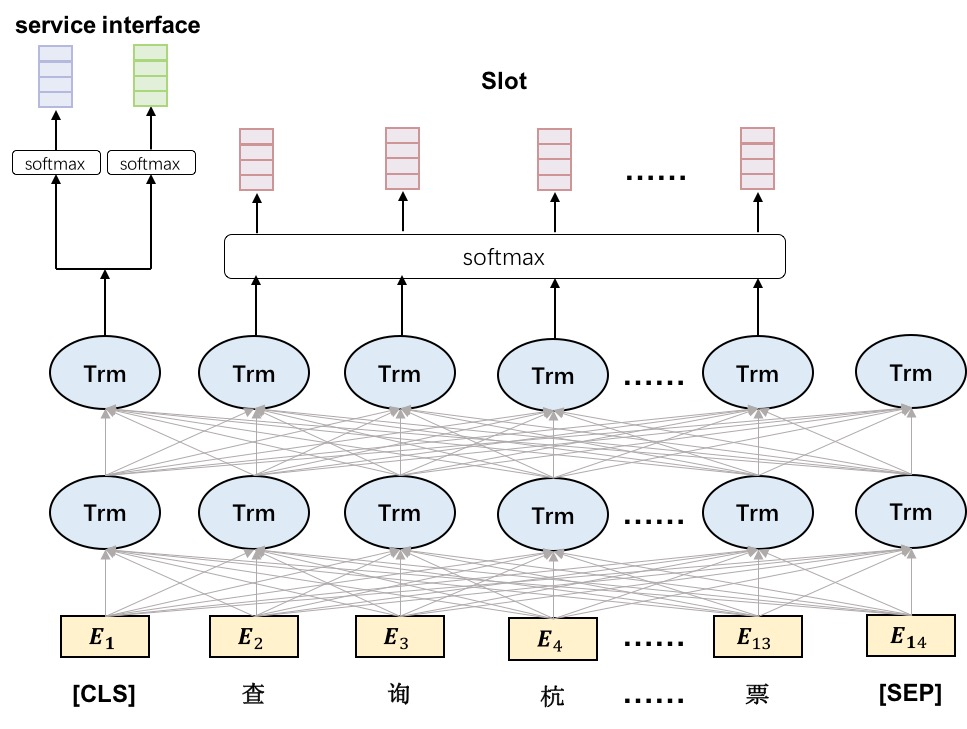
\includegraphics[width=15cm]{./images/bert-base.jpg}
  \caption{bert-base联合识别模型}
  \label{fig:bert-base}
\end{figure}

模型结构非常清晰,将用户语句按字向量序列输入bert模型编码,得到bert的输出$\mathbf{H}$=[$h_{1}$,$h_{2}$,\dots,$h_{n}$],
我们取bert输出的第一个向量,也就是特殊token([CLS])的隐藏状态作为两项分类任务的输入传给softmax层:
\begin{equation}
  y^{d}=\operatorname{softmax}\left(\mathbf{W}^{d} \boldsymbol{h}_{1}+\boldsymbol{b}^{d}\right)
\end{equation}
\begin{equation}
  y^{i}=\operatorname{softmax}\left(\mathbf{W}^{i} \boldsymbol{h}_{1}+\boldsymbol{b}^{i}\right)
\end{equation}
对于参数填充任务,将[$h_{2}$,\dots,$h_{n}$]隐层状态传入softmax层,以对插槽填充标签进行分类:
\begin{equation}
y_{n}^{s}=\operatorname{softmax}\left(\mathbf{W}^{s} \boldsymbol{h}_{n}+\boldsymbol{b}^{s}\right), n \in 2 \ldots N
\end{equation}
三项任务联合概率函数为:
\begin{equation}
  p\left(y^{d},y^{i}, y^{s} \mid \boldsymbol{x}\right)=p\left(y^{d} \mid \boldsymbol{x}\right) \left(y^{i} \mid \boldsymbol{x}\right) \prod_{n=1}^{N} p\left(y_{n}^{s} \mid \boldsymbol{x}\right)
  \end{equation}
  训练的目标是最大化正确标签的概率$p\left(y^{d},y^{i}, y^{s} \mid \boldsymbol{x}\right)$。

\subsection{bert-co-interactive联合识别模型}

为在co-interactive联合识别模型中引入bert,将其共享编码器换成bert拼接在attention层之前\ref{fig:bert-joint},模型其他结构与co-interactive模型
一致不再赘述,bert部分的参数采用fine-tuning的方式更新。
\begin{figure}[htbp]
  \centering
  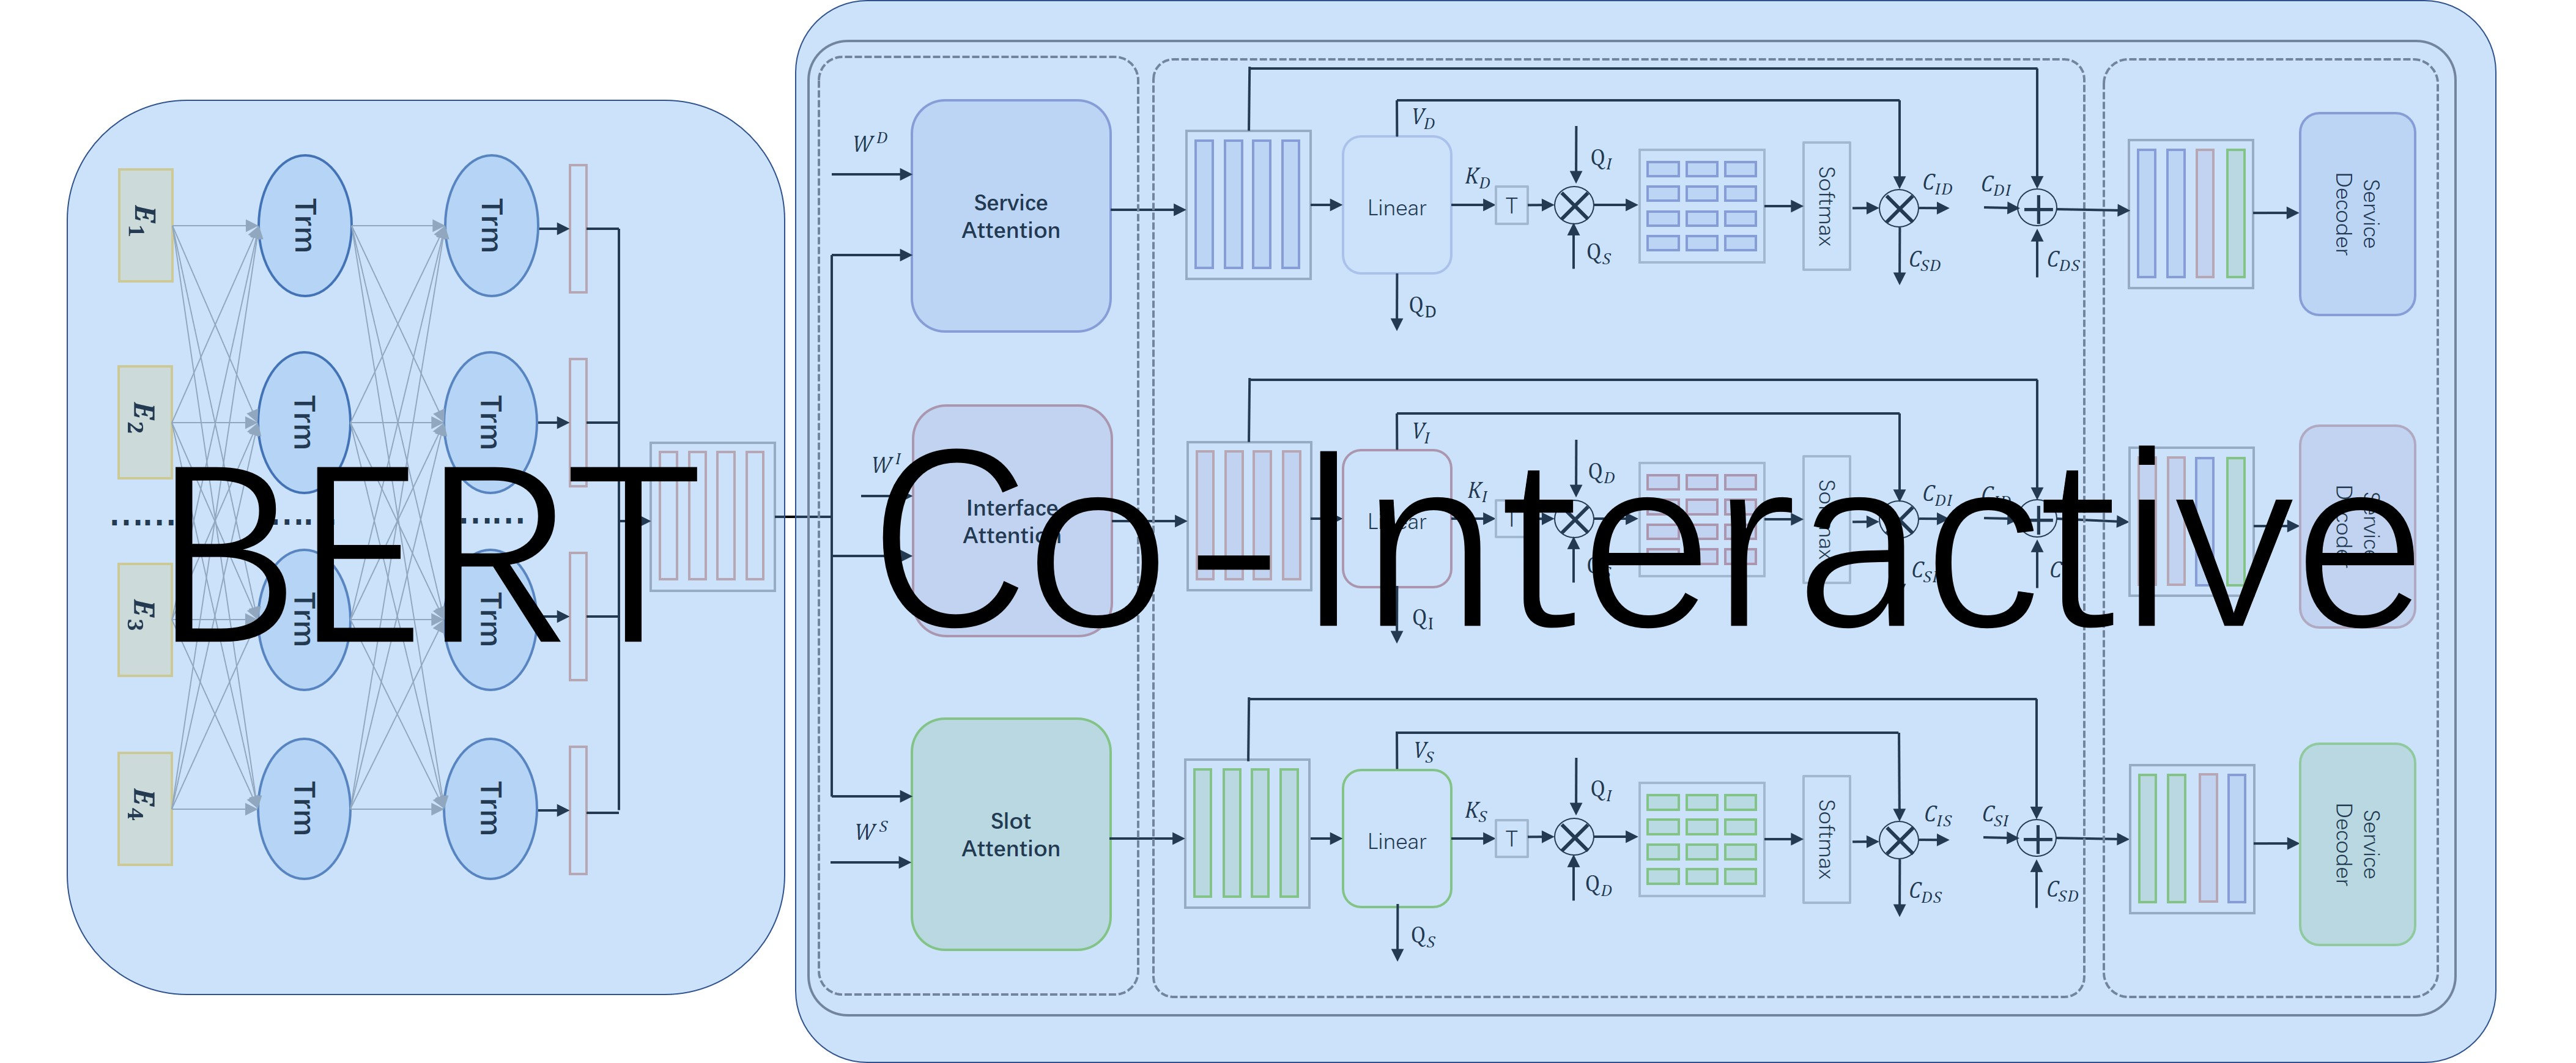
\includegraphics[width=14cm]{./images/bert-joint.jpg}
  \caption{引入bert交互式联合识别模型}
  \label{fig:bert-joint}
\end{figure}


% \section{结合ernie的模型}
\section{引入知识图谱}
与段落或文档不同,短文本输入做为信息源更加模糊,因为它们没有足够的上下文信息,这对语义理解造成了很大的挑战。
在本小节中,我们从外部知识源中检索知识,以增强短文本的语义表示。我们将概念性信息视为一种知识,并将其传入深度神经网络。
知识库(KB)中存在的重要语义关系,例如isA和isPropertyOf等,这些信息有助于理解短文本,尤其是模型在处理训练集中未出现的短语时。
例如,给定一个简短的文本“播放林俊杰的江南”,未引入KB的模型可能会将林俊杰当作普通人名,而无法学习到林俊杰是歌手,如果KB中林俊杰是歌手的知识
能输入到神经网络中,将有助于将文本归类于“music”服务。

如果将概念信息简单地集成到深度神经网络中,会存在一个问题:在概念化短文本时,由于实体的歧义或KB的噪声,很容易引入一些不正确或不想关的概念。
例如,在文本“查询苹果公司今日股价”,我们会从KB获得“苹果”的“水果”和“手机”概念。显然,这里的“水果”并不是一个恰当的概念,这是由实体的歧义造成的。
为了解决这个问题,衡量知识的重要性,我们使用C-T注意力(concept,text)来衡量短文本及其相应概念之间的语义相似性,
从而模型会将更大的权重分配给概念“手机”,因为它在语义上与短文本更接近,而不是概念“水果”。
借助概念性信息对短文本进行数据增强,与之前的方法不同,使模型像人类一样有了很多先验知识。如图\ref{fig:kg}所示,在bert-co-interactive联合识别模型
的基础上,本小节对其编码层进行了改进:
% 我们引入注意力机制,并提出了具有知识动力注意的深层短文本分类(STCKA)。

% 为了衡量知识的重要性,我们介绍了注意力机制,并提出了基于知识动力的注意力的短文本分类(STCKA),利用对短文本(CST)的关注和对概念集(C-CS)的关注来从两个方面获得概念的重要性。


% 我们借助诸如YAGO(Suchanek,Kasneci和Weikum 2008)和Freebase(Bollacker等人2008)之类的显式KB来丰富短文本的语义表示。
% 这允许模型从外部知识源检索知识,该知识未在短文本中明确说明,但与分类有关。如S1所示,作为一种知识的概念信息有助于分类。
% 因此,我们利用isA关系,并通过概念化1将每个短文本与其相关概念以KB关联。之后,我们将概念信息作为先验知识整合到深度神经网络中。


% 我们的模型包含四个模块。知识检索模块从知识库中检索与短文本相关的概念信息。
% 输入嵌入模块利用短文本的字符和单词级别功能来生成单词和概念的表示形式。
% 短文本编码模块通过自我注意对短文本进行编码,并产生短文本表示q。
% 知识编码模块对概念向量应用两种注意机制,以获得概念表示p。
% 接下来,我们将p和q连接起来以融合短文本和概念信息,这些信息将被馈送到完全连接的层中。
\begin{figure}[htbp]
  \centering
  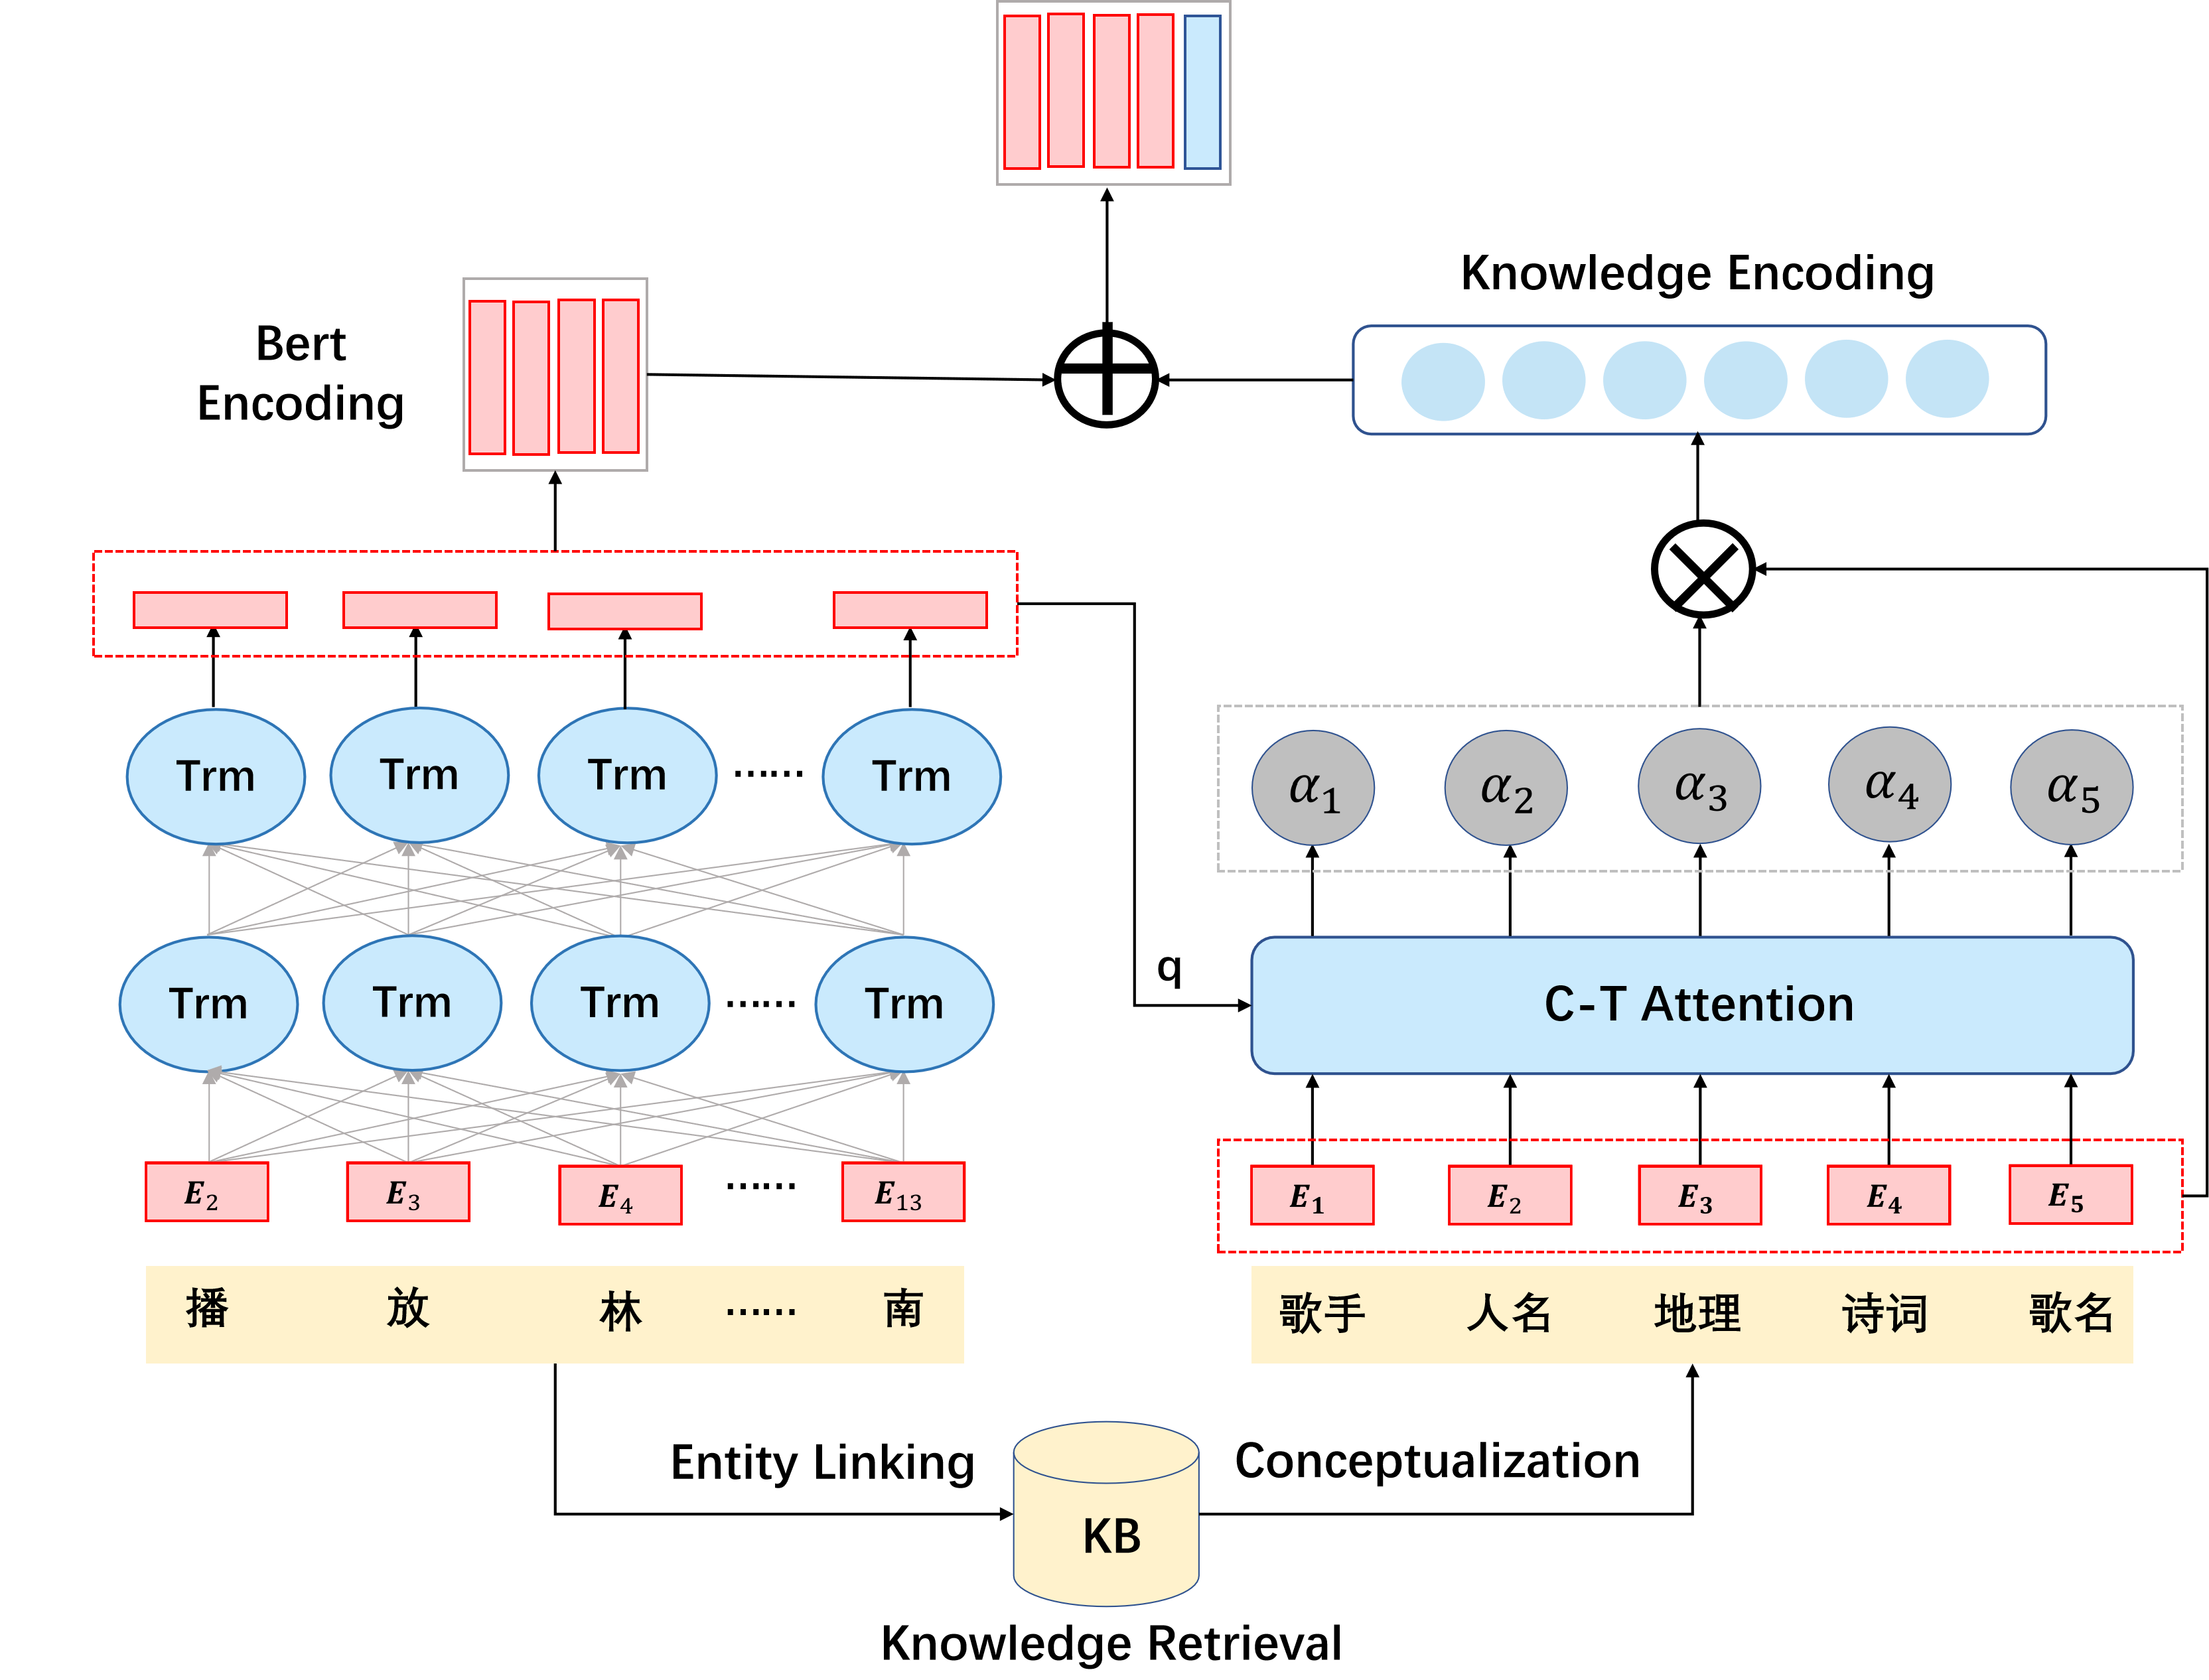
\includegraphics[width=16cm]{./images/kg.png}
  \caption{引入知识图谱的编码层}
  \label{fig:kg}
\end{figure}
(1)知识检索

该模块的目的是从知识库中检索相关知识,语义关系主要选用isA,isPropertyOf两种,给定一个简短的文本,希望找到与其相关的概念集C。
可通过两个主要步骤来实现此目的:实体链接和概念化。
实体链接是NLP中的一项重要任务,用于识别短文本中提到的实体\cite{moro2014entity},
本文通过利用现有的实体链接解决方案,获得了短文本的实体集E\cite{chen2018short}。
然后,对于每个实体e $\in$ E,我们通过概念化从CN-Probase现有知识库中获取其概念信息。
例如,给定一个用户输入文本“播放林俊杰的江南”,通过实体链接可获得实体集E = {林俊杰,江南}。
然后,我们将实体集E概念化,并从CN-Probase获得其概念集C = {人名,歌手,地理,诗词,歌名}。

(2)C-T attention
如前所述,简单地将所有概念信息集成到深度神经网络中,会存在实体的歧义或KB的噪声的问题,因此使用C-T注意力机制。
给定大小为m的概念集C,计为($c_1$,$c_2$,$\dots$,$c_m$),其中$c_i$是第i个概念向量,我们旨在产生概念集C的向量表示p。 
为了减少由于实体的歧义或KB噪声而引入的一些不正确概念,使用以下公式来计算C-T注意力以衡量第i个概念与文本表示向量q之间的语义相似性:
\begin{equation}
\alpha_{i}=\operatorname{softmax}\left(w_{1}^{T} f\left(W\left[c_{i} ; q\right]+b\right)\right)
\end{equation}
其中q是bert输出的矩阵经过max-pooling处理得到的用户输入语句向量级表示,
$\alpha_{i}$表示第i个概念到短文本的注意权重,较大的$\alpha_{i}$表示第i个概念在语义上与短文本更相似,
f采用非线性激活函数双曲线正切变换,W和b是训练参数。
\begin{equation}
p=\sum_{i=1}^{m} a_{i} c_{i}
\end{equation}
最后通过加权求和得到knowledge encoding的向量表示p,将p和bert输出的矩阵连接得到引入知识的编码结果,
后续会传入co-interactive层,其结构已经在之前介绍过,不再赘述。

\section{本章小结}
本章利用任务之间存在的强关联性,将服务分类、接口分类和参数填充三项任务做了联合识别,包括单向信息流的联合和交互式联合两种尝试,
同时引入预训练模型bert对模型进行优化,在此基础上引入知识库丰富输入语句的语义信息,得到了不错的效果。


% \chapter{实验与讨论}

\section{实验数据集与预处理}
\subsection{实验数据集}
本文作者实验开始前调研了与本文任务相关的数据集,调研结果发现可用于跨界服务平台的高质量中文语料数据集相对匮乏,
且如科大讯飞、阿里小蜜等有着海量有商业价值数据的公司没有公开数据集。为此,我们选择在已有数据集上做标注补充和数据扩展,构建了跨界服务相关的中文
语料数据集。

\begin{figure}[htbp]
    \centering
    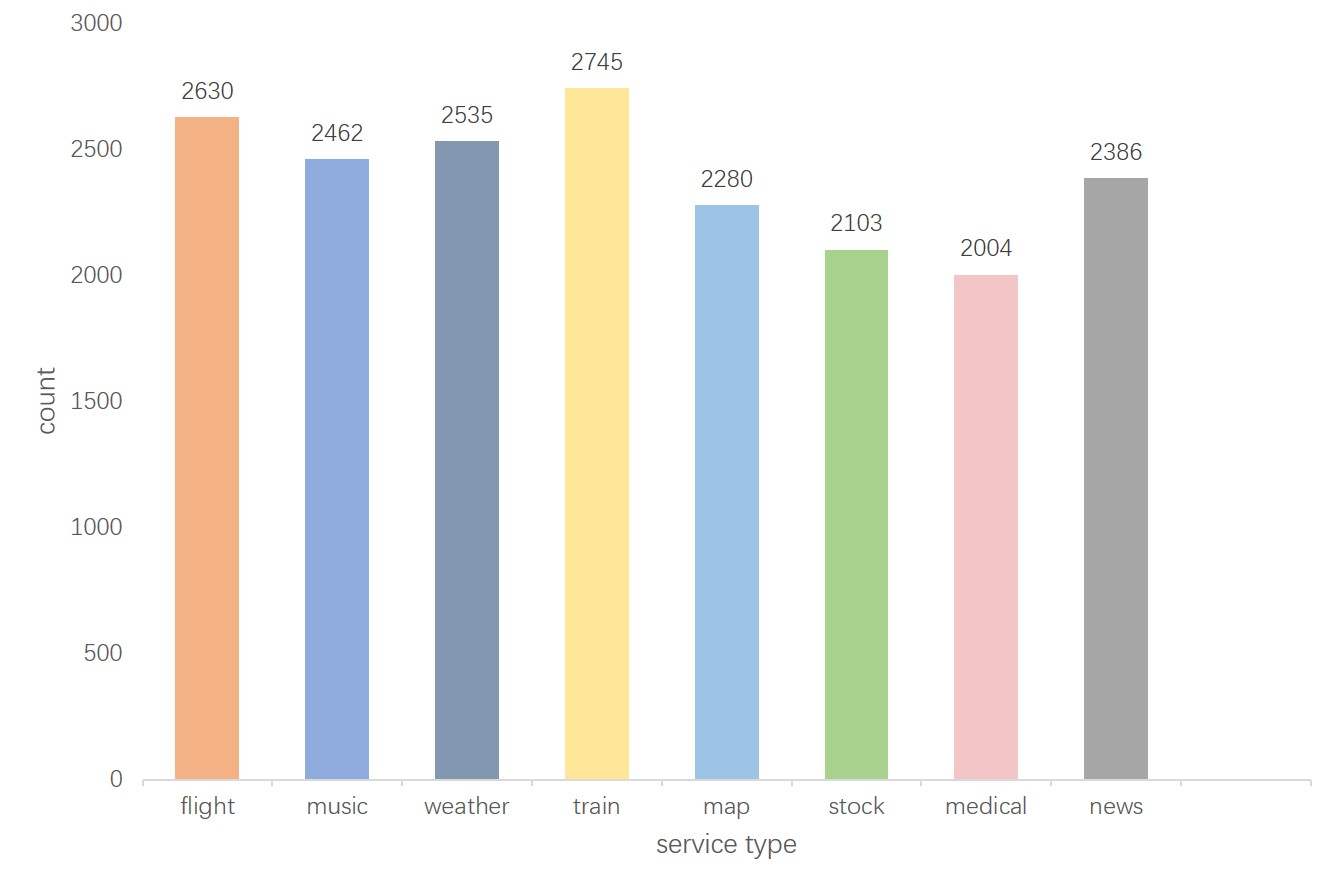
\includegraphics[width=15cm]{./images/count.jpg}
    \caption{数据集分布图}
    \label{fig:count}
  \end{figure}

SMP2019中文人机对话技术评测自然语言理解任务中提供了SMP2019ECDT数据集,其中主要包括垂直类,闲聊类和知识问答,我们结合跨界服务网络系统内部常用
服务,从垂直类中选择部分数据做数据扩充。本文筛选了跨界服务网络系统中用户使用较多的几类服务的语料信息,包括“航班flight”,“音乐music”,
“天气weather”,“火车train”,“地图map”,“股票stock”,“医疗medical”,“新闻news”共八大类服务,再根据这些服务的接口构建接口类别的全集,例如“query”,“play”,“order”等。
同时确定了服务接口以后,服务接口调用
时的参数(语义槽)也就确定了,如“songName”,“singer”,“startCity”,“endCity”等,因为接口和服务参数都是和服务强相关的。举例来说,当服务类型被判定为
“天气weather”时,接口类型在系统内限定为“query”,参数(语义槽)限定为“city”。

SMP2019ECDT数据集中与跨界服务平台系统内八大服务相关的数据量并不大,因此本文对原有数据集做了扩充。扩充工作主要分为两部分:横向扩充和纵向扩充,横向
扩充的原理来源于同一语义的句子不同人的表述会不同,例如“杭州具体天气怎么样?”和“杭州今天多少度?”表达了想要调用天气服务的相同意愿,因此考虑对同种语义的句子做横向扩充,这里我们借助
了百度和必应(微软bing)两大搜索引擎的搜索联想补全功能。横向扩充完的句子标签中的服务类别和接口类别不用变,只需要修改语义槽标注。
如图\ref{fig:baidu},\ref{fig:bing}所示,想要扩展火车服务的查询接口的语料数据,再搜索引擎输入“成都到杭州火车”,利用搜索引擎的联想补全功能
达到扩充的目的。


  \begin{figure}[htbp]
    \subfloat[搜索引擎百度]{
      \centering
    
\includegraphics[width=8cm]{./images/baidu.png}
    
    \label{fig:baidu}
    }
    \subfloat[搜索引擎bing]{
      \centering
    
\includegraphics[width=8cm]{./images/bing.png}
    \label{fig:bing}
    }
    \caption{数据横向扩充图}
    
    \end{figure}

数据集纵向扩充是组织跨界服务课题组和实验室同学填写问卷,让被调研者输入相应服务的查询语句,收集起来对语句进行人工标注,完成数据集的扩容。
每个人对同一语义的表达会有差异,有差异的数据对训练出泛化能力好的数据是大有裨益的。最终经过课题组同学的努力,共构建了19145条数据组成实验
数据集,每条数据都包含服务类别标签、接口类别标签和参数(语义槽)标签,并将60\%数据作为训练集,20\%数据作为验证集,20\%数据作为测试集。

% \subsection{预处理}

\section{评价指标}
评价指标用于评估模型的性能,对于服务分类任务,本文采用准确率(Accuracy)来评估模型;对于接口分类
任务,同样采用准确率(Accuracy)来评估模型;对于参数(语义槽)填充任务,采用$F_1$值来评估模型。同时引入
句子准确率(Sentence Accuracy)作为更严格的指标来评估模型,即一个句子只有在三项任务同时正确时才会被计入
句子准确率中。

 \begin{table}[htb]
      \centering
      \caption{服务类型混淆矩阵}
      \label{tab:hunxiao}
  \begin{tabular}{c|c|c|c|c|c|c|c|c|c}
    \toprule
    \multicolumn{2}{c|}{\multirow{2}{*}{}}&
    \multicolumn{8}{c}{预测值}\\
    \cline{3-10}
    \multicolumn{2}{c|}{}&flight & music & weather & train & map &stock &medical & news \\
     \hline
     \multirow{8}{*}{真实值}&
     flight&$n_1$&$n_2$&$n_3$&$n_4$&$n_5$&$n_6$&$n_7$&$n_8$\\
     \cline{2-10}
     \multicolumn{1}{c|}{}&music&$n_{9}$&$n_{10}$&$n_{11}$&$n_{12}$&$n_{13}$&$n_{14}$&$n_{15}$&$n_{16}$\\
     \cline{2-10}
     \multicolumn{1}{c|}{}&weather&$n_{17}$&$n_{18}$&$n_{19}$&$n_{20}$&$n_{21}$&$n_{22}$&$n_{23}$&$n_{24}$\\
     \cline{2-10}
     \multicolumn{1}{c|}{}&train&$n_{25}$&$n_{26}$&$n_{27}$&$n_{28}$&$n_{29}$&$n_{30}$&$n_{31}$&$n_{32}$\\
     \cline{2-10}
     \multicolumn{1}{c|}{}&map&$n_{33}$&$n_{34}$&$n_{35}$&$n_{36}$&$n_{37}$&$n_{38}$&$n_{39}$&$n_{40}$\\
     \cline{2-10}
     \multicolumn{1}{c|}{}&stock&$n_{41}$&$n_{42}$&$n_{43}$&$n_{44}$&$n_{45}$&$n_{46}$&$n_{47}$&$n_{48}$\\
     \cline{2-10}
     \multicolumn{1}{c|}{}&medical&$n_{49}$&$n_{50}$&$n_{51}$&$n_{52}$&$n_{53}$&$n_{54}$&$n_{55}$&$n_{56}$\\
     \cline{2-10}
     \multicolumn{1}{c|}{}&news&$n_{57}$&$n_{58}$&$n_{59}$&$n_{60}$&$n_{61}$&$n_{62}$&$n_{63}$&$n_{64}$\\
    \bottomrule
    \end{tabular}
  \end{table}

  以服务类别标签的混淆矩阵\ref{tab:hunxiao}为例介绍以上指标的计算方法,设样本数据总量是N。
  准确率(Accuracy)是最直观的性能指标,它是正确预测的观测值与总观测值的比率,如果具有很高的准确率,可以认为模型是很好的:
  \begin{equation}
  % \text {Accuracy}(\text {health})=\frac{\sum_{i=8}^{14} n_{i}}{N}
  \text {Accuracy}=\frac{n_1+n_{10}+n_{19}+n_{28}+n_{37}+n_{46}+n_{55}+n_{64}}{N}
\end{equation}
精确度(Precision)是正确预测的该类样本与总的预测为该类样本的观察值之比,多用于二分类问题,对于文本分类这样的多分类问题,可以单独取一个类别做计算,以天气类别为例:
\begin{equation}
  \text {Precision}(\text {weather})=\frac{n_{19}}{n_3+n_{11}+n_{19}+n_{27}+n_{35}+n_{43}+n_{51}+n_{69}}
\end{equation}
召回率(Recall)是正确预测的该类样本与实际为该类的样本总量的比率,多用于二分类问题,对于文本分类这样的多分类问题,可以单独取一个类别做计算,以天气类别为例:
\begin{equation}
  \text {Recall}(\text {weather})=\frac{n_{19}}{\sum_{i=17}^{24} n_{i}}
\end{equation}
F1值是精确度和召回率的调和平均值,直观上它不如准确性容易理解,但是F1通常比准确性更有用,尤其是在类分布不均匀的情况下:
\begin{equation}
  F_1=\frac{2 \times Precision \times Recall}{ Precision + Recall}
  % F_{1}=\frac{2 \times \text {Precision } \times \text { Recall}}{\text {Precision }+\text { Recall}}
\end{equation}

\section{实验设置}
\subsection{实验环境}
本文的实验环境是实验室服务器,操作系统为Ubuntu 16.04.4系统,集成开发环境选用Pycharm使用Python语言利用PyTorch框架编程。
关于实验室机器硬件配置,中央处理器为Intel(R) Xeon(R) CPU E5-2603 v3 @ 1.60GHz,图形处理器为GeForce RTX 2080Ti。

\begin{table}[htb]
  \centering
  \caption{实验环境}
  \label{tab:huanjing}
\begin{tabular}{c|c}
\hline
实验环境&配置参数\\
\hline
操作系统&Ubuntu 16.04.4\\
编程语言&python 3.6\\
IDE&Pycharm\\
模型框架&PyTorch\\
\hline
\end{tabular}
\end{table}

\subsection{超参数设置}
超参数的调整主要利用验证集依靠控制变量法来寻找最优的超参数值,同一实验进行多次训练取最优。例如,卷积层的激活函数本文对比了ReLu、Tanh、PReLU,
CNN层卷积核高度对比了2,3,4三种,卷积核的数量进行了16,32,64,128四种不同的实验等,比较不同超参数对实验结果的影响。
ATT-CLSTM模型和Trans-CLSTM模型中CNN层最终确定的超参数值如表\ref{tab:cnnPara}所示,
引入预训练的模型最终确定的超参数值如表\ref{tab:bertPara}所示,

\begin{table}[htb]
  \centering
  \caption{CNN层相关参数选择}
  \label{tab:cnnPara}
\begin{tabular}{cc|cc}
\hline
参数名称&值&参数名称&值\\
\hline
卷积核高度&2,3&卷积核数量&64\\
learning rate&0.002&batch size&128\\
池化层方法&k-max polling&epochs &60\\
Optimizer&Adam&&\\
\hline
\end{tabular}
\end{table}

\begin{table}[htb]
  \centering
  \caption{引入预训练的模型相关参数选择}
  \label{tab:bertPara}
\begin{tabular}{cc|cc}
\hline
参数名称&值&参数名称&值\\
\hline
learning rate&5e-4&batch size&64\\
Optimizer&Adam&epochs &20\\
堆叠层数N&2&&\\
\hline
\end{tabular}
\end{table}

\section{实验设计}
本文对前两章提到的所有模型都进行了实验,虽然模型数量较多,但总的来说可分为两类:基于词向量的模型和引入预训练的模型。
\subsection{基于词向量的模型}
前文提到的ATT-CLSTM模型、Trans-CLSTM模型、BLSTM-ATT-CRF模型均是基于词向量的模型,实验流程类似。
第一步输入句子经过分词处理得到词序列,接着利用word2vec将词语向量化输入神经网络训练。训练集数据用于模型的拟合,验证集数据用于对模型超参数的调整以及对模型性能做初步判定,
测试集用来评估模型最终的泛化能力。测试阶段加载训练好的模型参数,数据输入进入网络得到预测结果。
\begin{figure}[htbp]
  \centering
  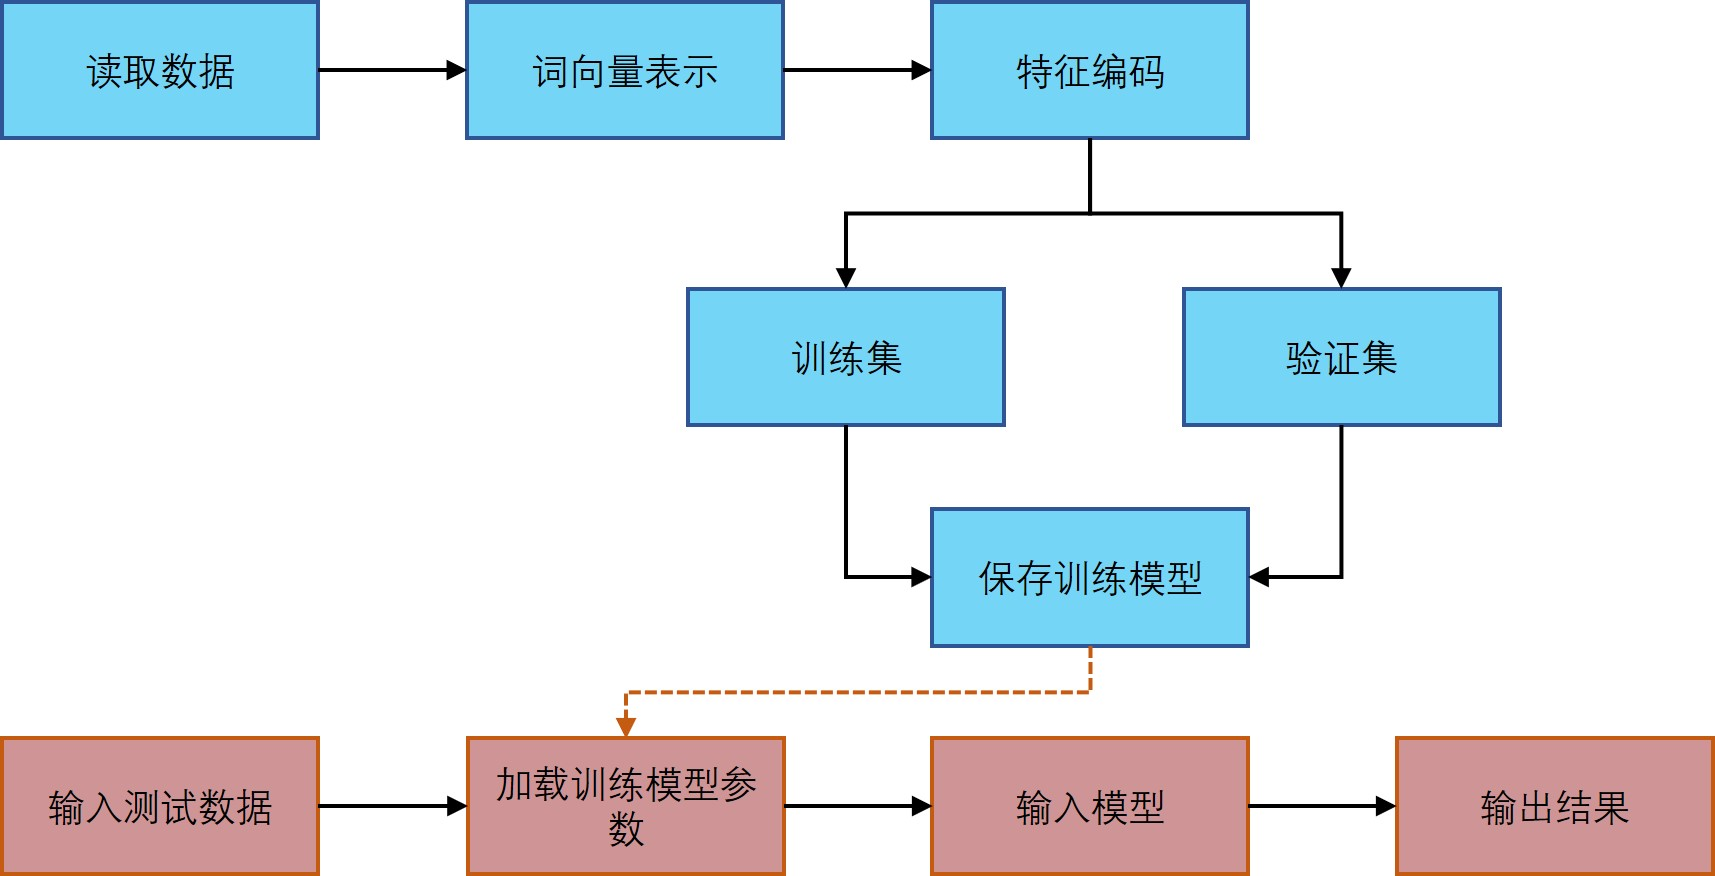
\includegraphics[scale=0.4]{./images/word2vecTrain.jpg}
  \caption{基于词向量模型的实验流程}
  \label{fig:word2vecTrain}
\end{figure}

\subsection{引入预训练的模型}
前文提到的slot-oriented联合识别模型、co-interactive联合识别模型、bert-base联合识别模型、bert-co-interactive联合识别模型均属于结合预训练的模型,实验流程类似。
首先加载预训练模型的参数,输入句子的字序列向量进入网络训练。训练集数据用于模型的拟合以及对预训练模型进行微调(fine-tuning),验证集数据用于对模型超参数的调整以及对模型性能做初步判定,
测试集用来评估模型最终的泛化能力。测试阶段加载训练好的模型参数和预训练参数,数据输入进入网络得到预测结果。
\begin{figure}[htbp]
  \centering
  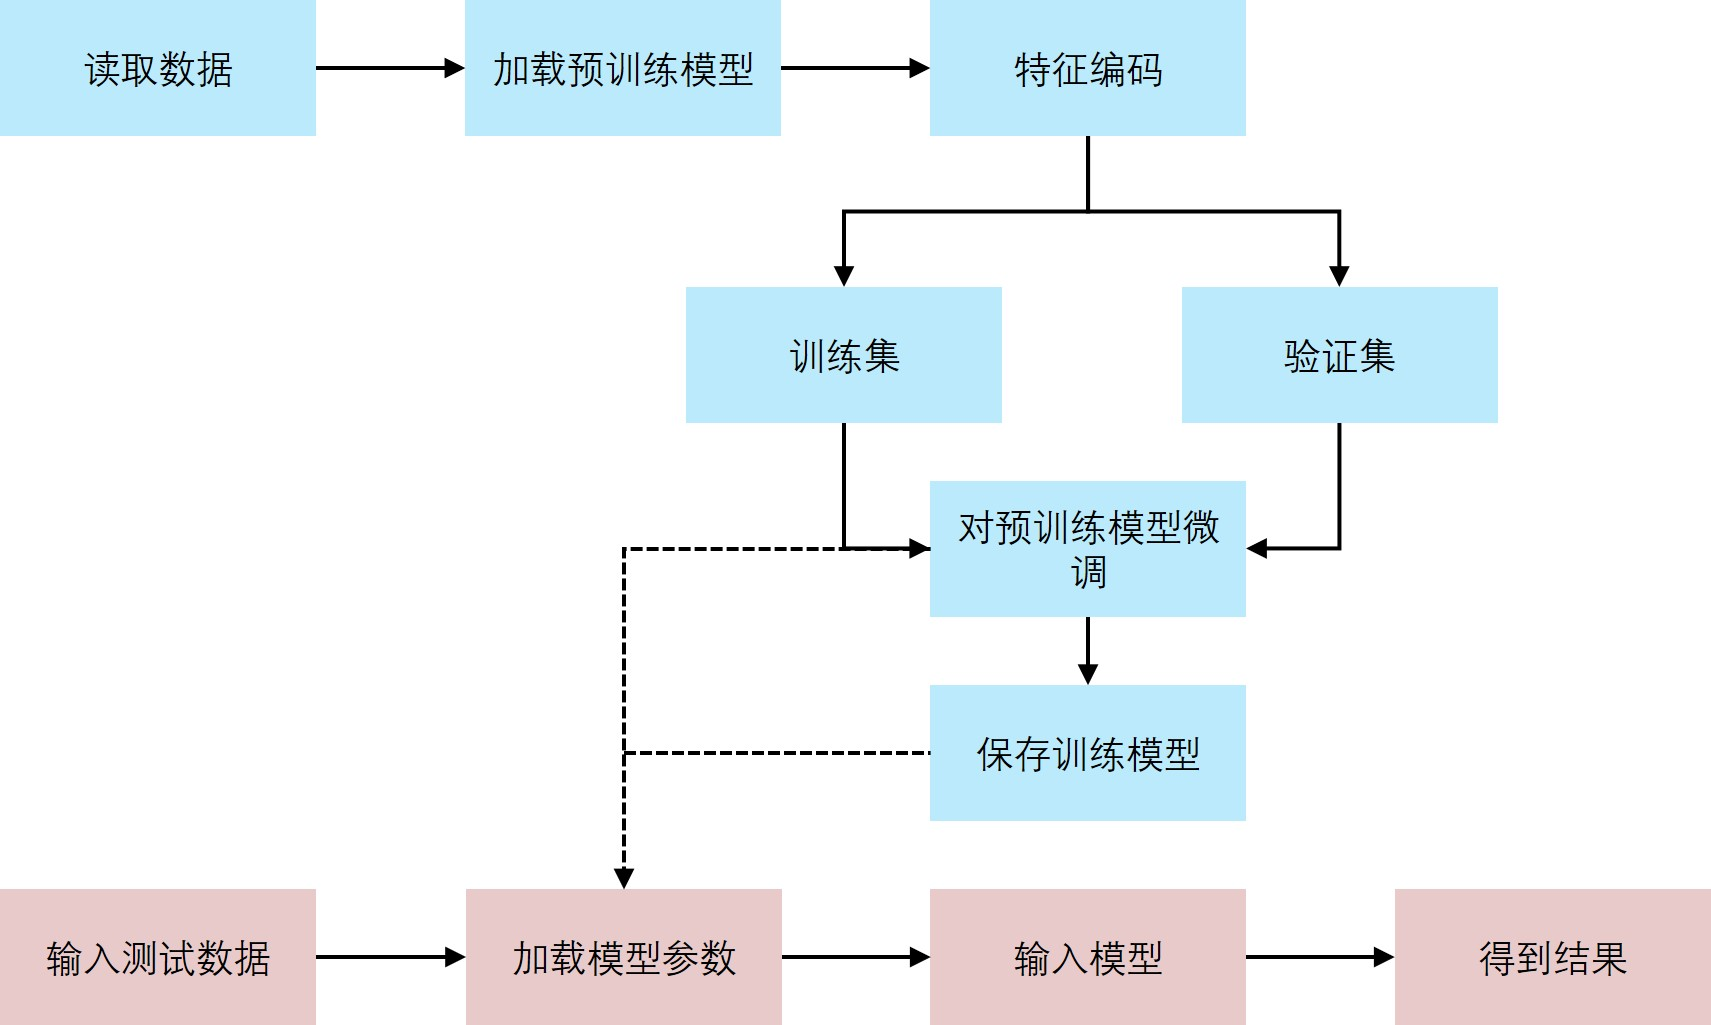
\includegraphics[scale=0.4]{./images/bertTrain.jpg}
  \caption{引入预训练模型的实验流程}
  \label{fig:bertTrain}
\end{figure}


\section{实验结果与分析}

\begin{figure}[htbp]
  % \centering
  % \hspace{-7mm}
  \subfloat[ATT-CLSTM loss值变化曲线]{
  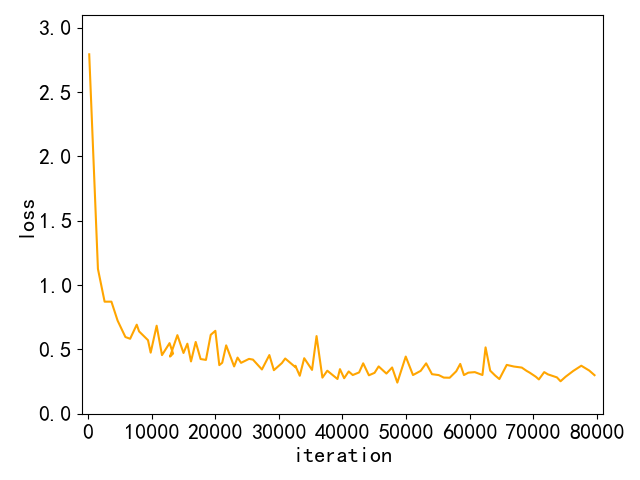
\includegraphics[width=8cm]{./images/bad.png}
  \label{fig:88888}
  }
  % \hspace{5pt}
    % \hspace{+5mm}
  \subfloat[BERT-base loss值变化曲线]{
  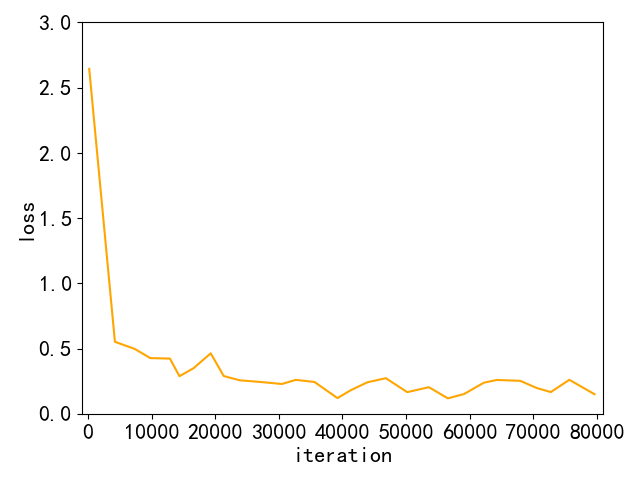
\includegraphics[width=8cm]{./images/good.png}
  \label{fig:88}
  }
  \caption{训练集loss值变化曲线}
  \label{fig:loss}
  \end{figure}

本实验模型较多且多数模型loss曲线走势相近,我们从结果中选择两类
有代表性的曲线走势展开分析,分别是基于词向量模型的ATT-CLSTM和基于bert的BERT-base,它们的损失函数Loss曲线变化如图\ref{fig:loss}所示,
可以看到经过多轮迭代后模型得到充分训练并趋于收敛,但结合了预训练模型的BERT-base相比于词向量的模型loss在收敛时震荡更小,收敛更快,最终结果也更优。

\begin{figure}[htbp]
  % \centering
  % \hspace{-7mm}
  \subfloat[服务Service分类的accuracy曲线]{
  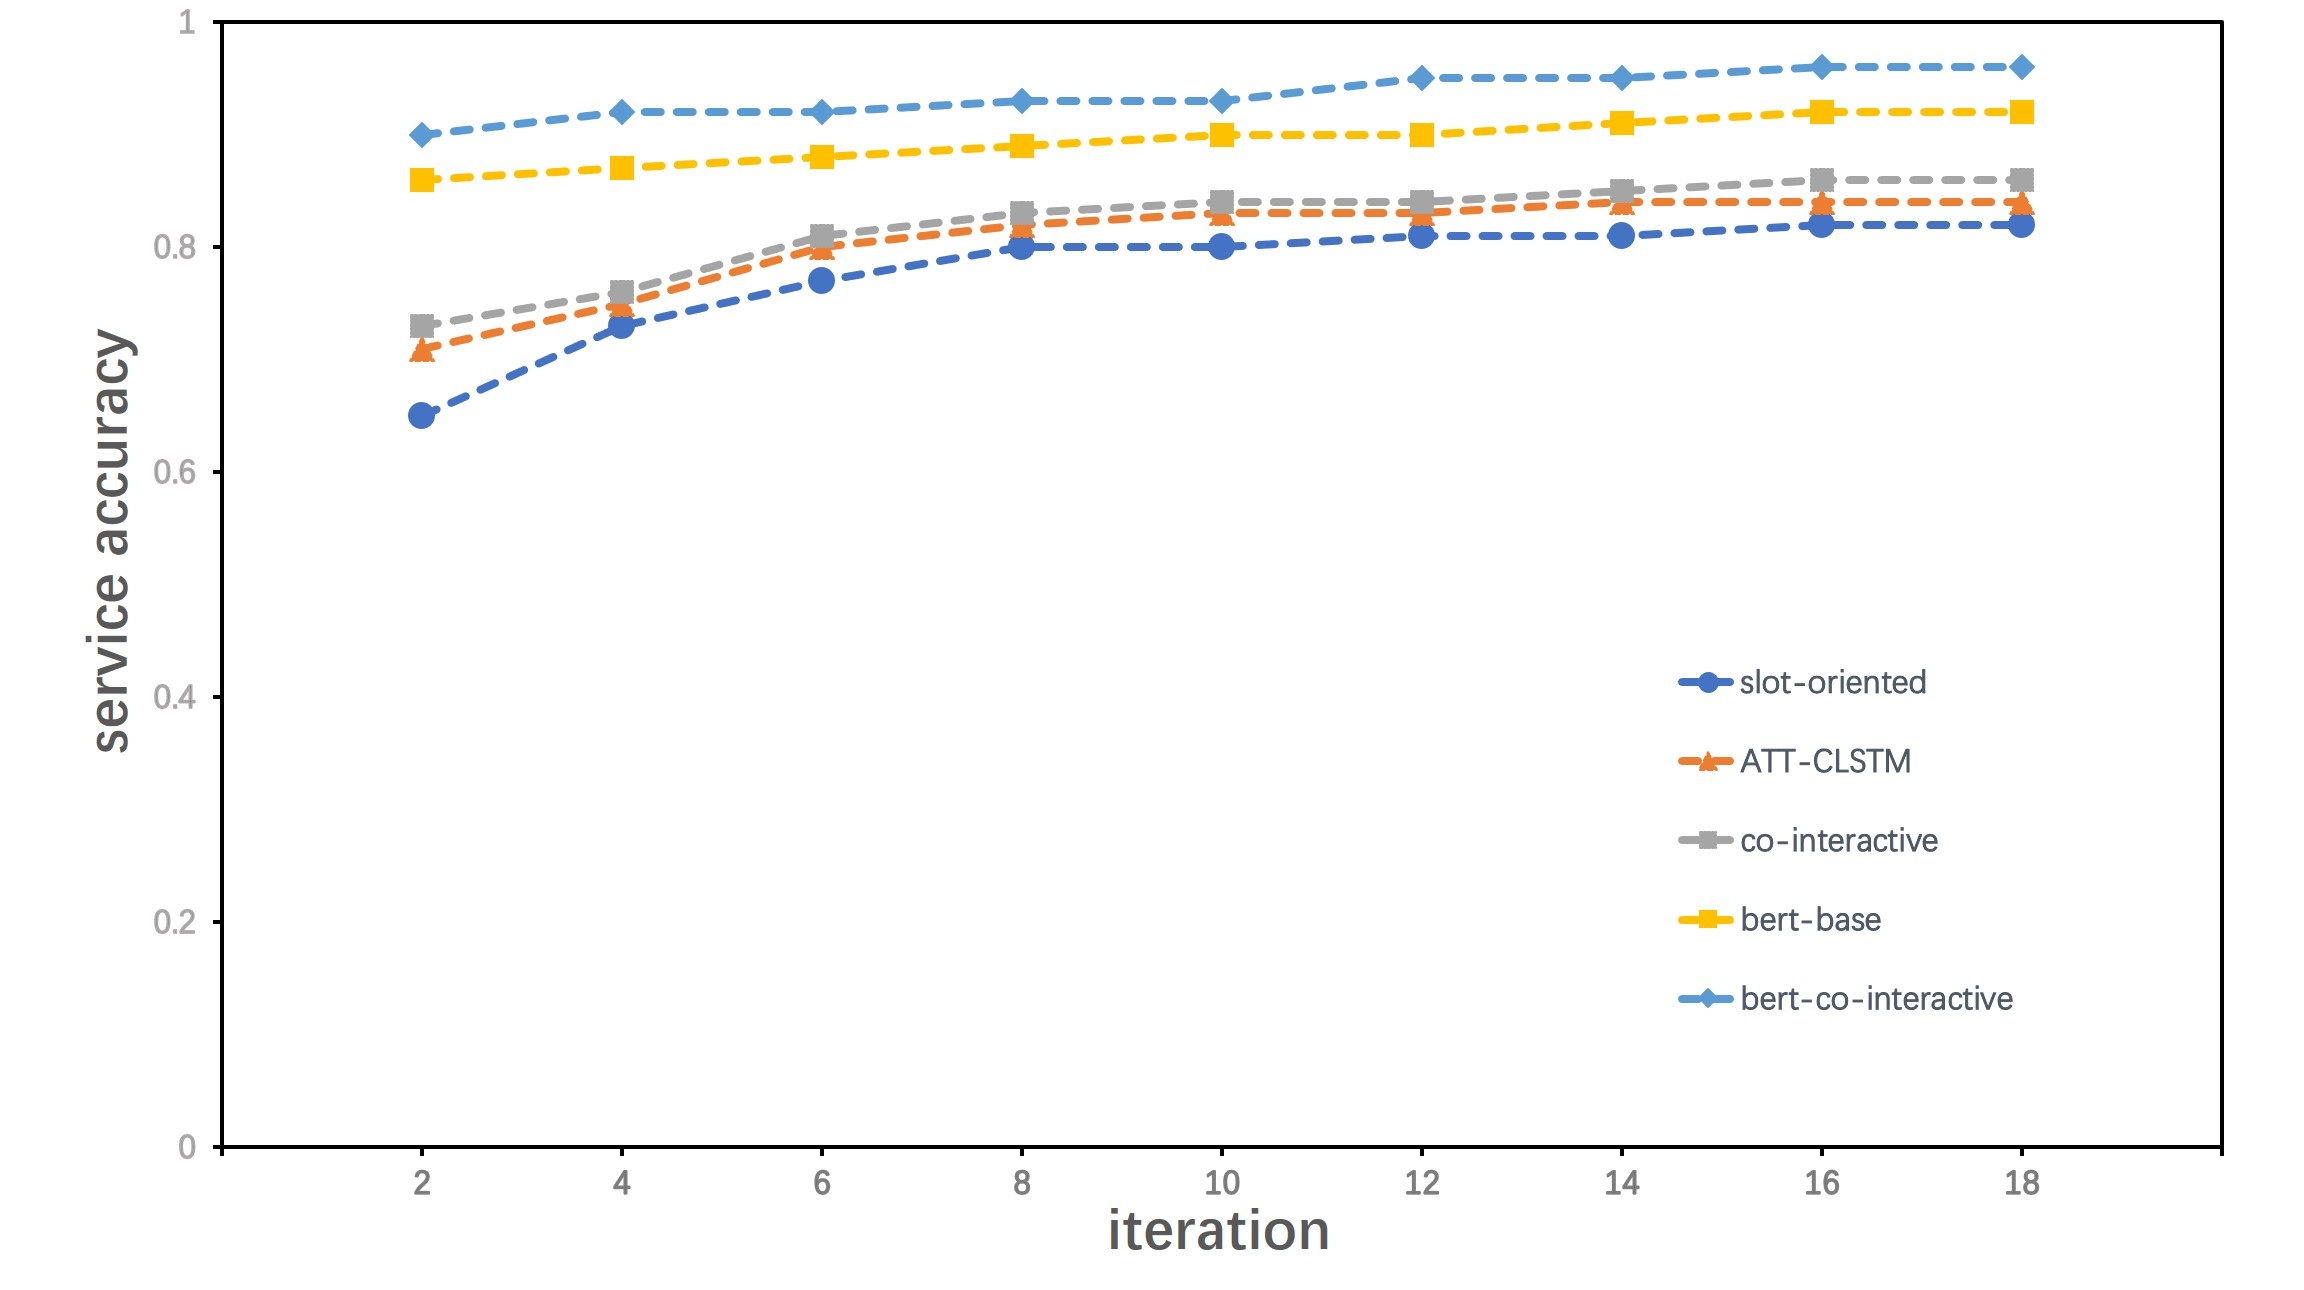
\includegraphics[width=8cm]{./images/serviceAccuracy.jpg}
  \label{fig:serviceAccuracy}
  }
  % \hspace{5pt}
    % \hspace{+5mm}
  \subfloat[接口Interface分类的accuracy曲线]{
  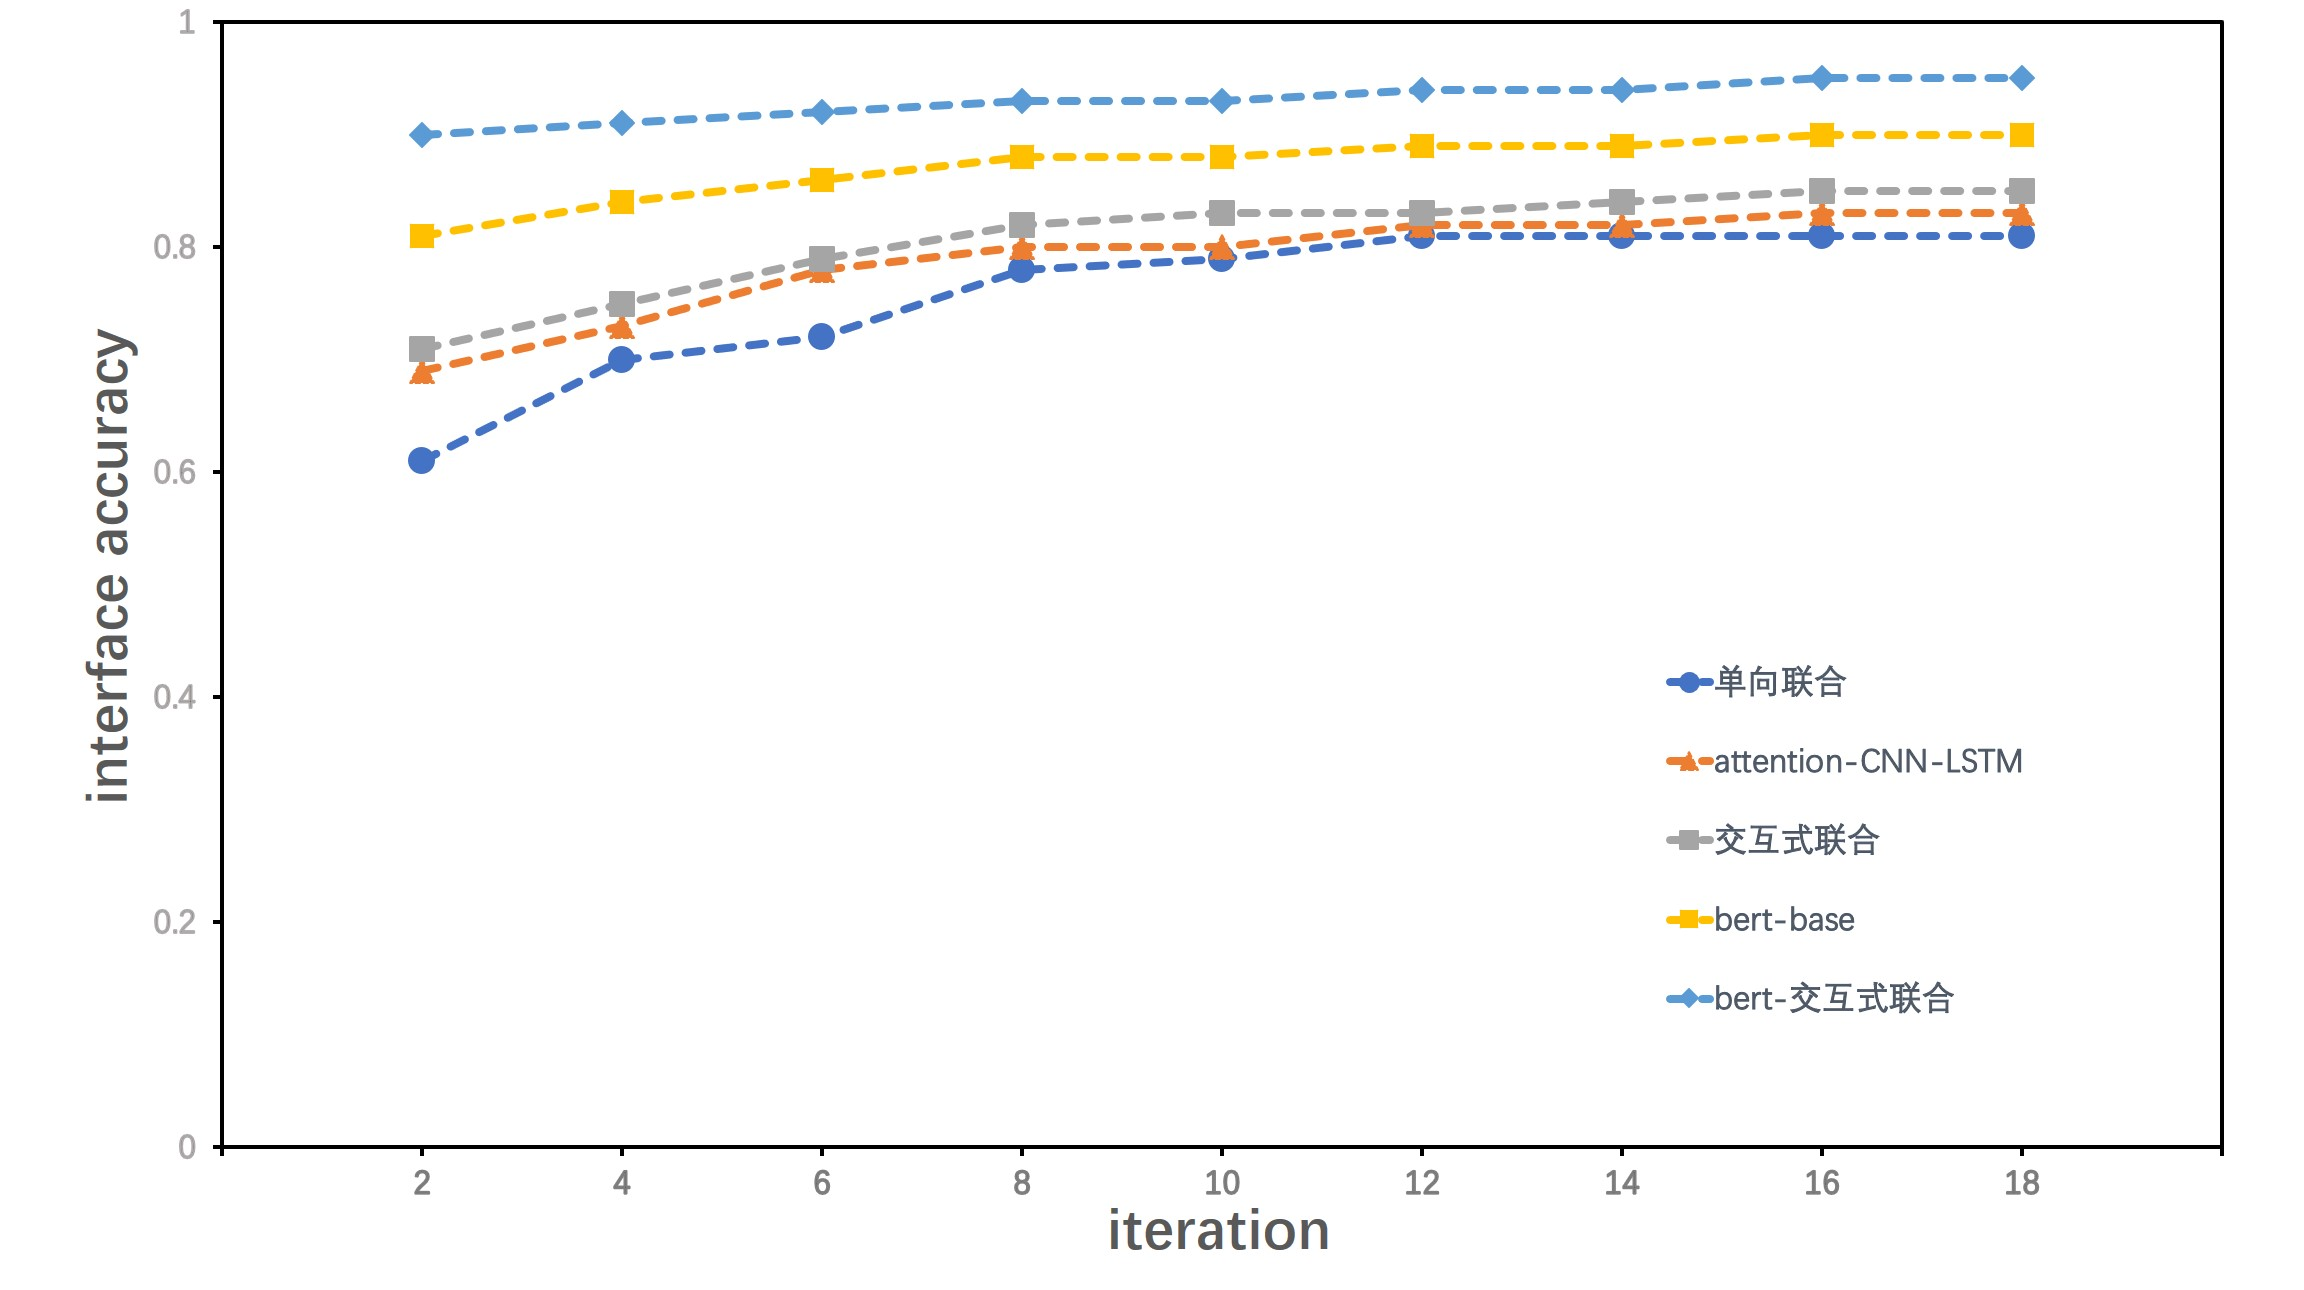
\includegraphics[width=8cm]{./images/interfaceAccuracy.jpg}
  \label{fig:interfaceAccuracy}
  }\\
  % \hspace{5pt}
  %  \hspace{-7mm}
  \subfloat[语义槽填充的$F_1$曲线]{
  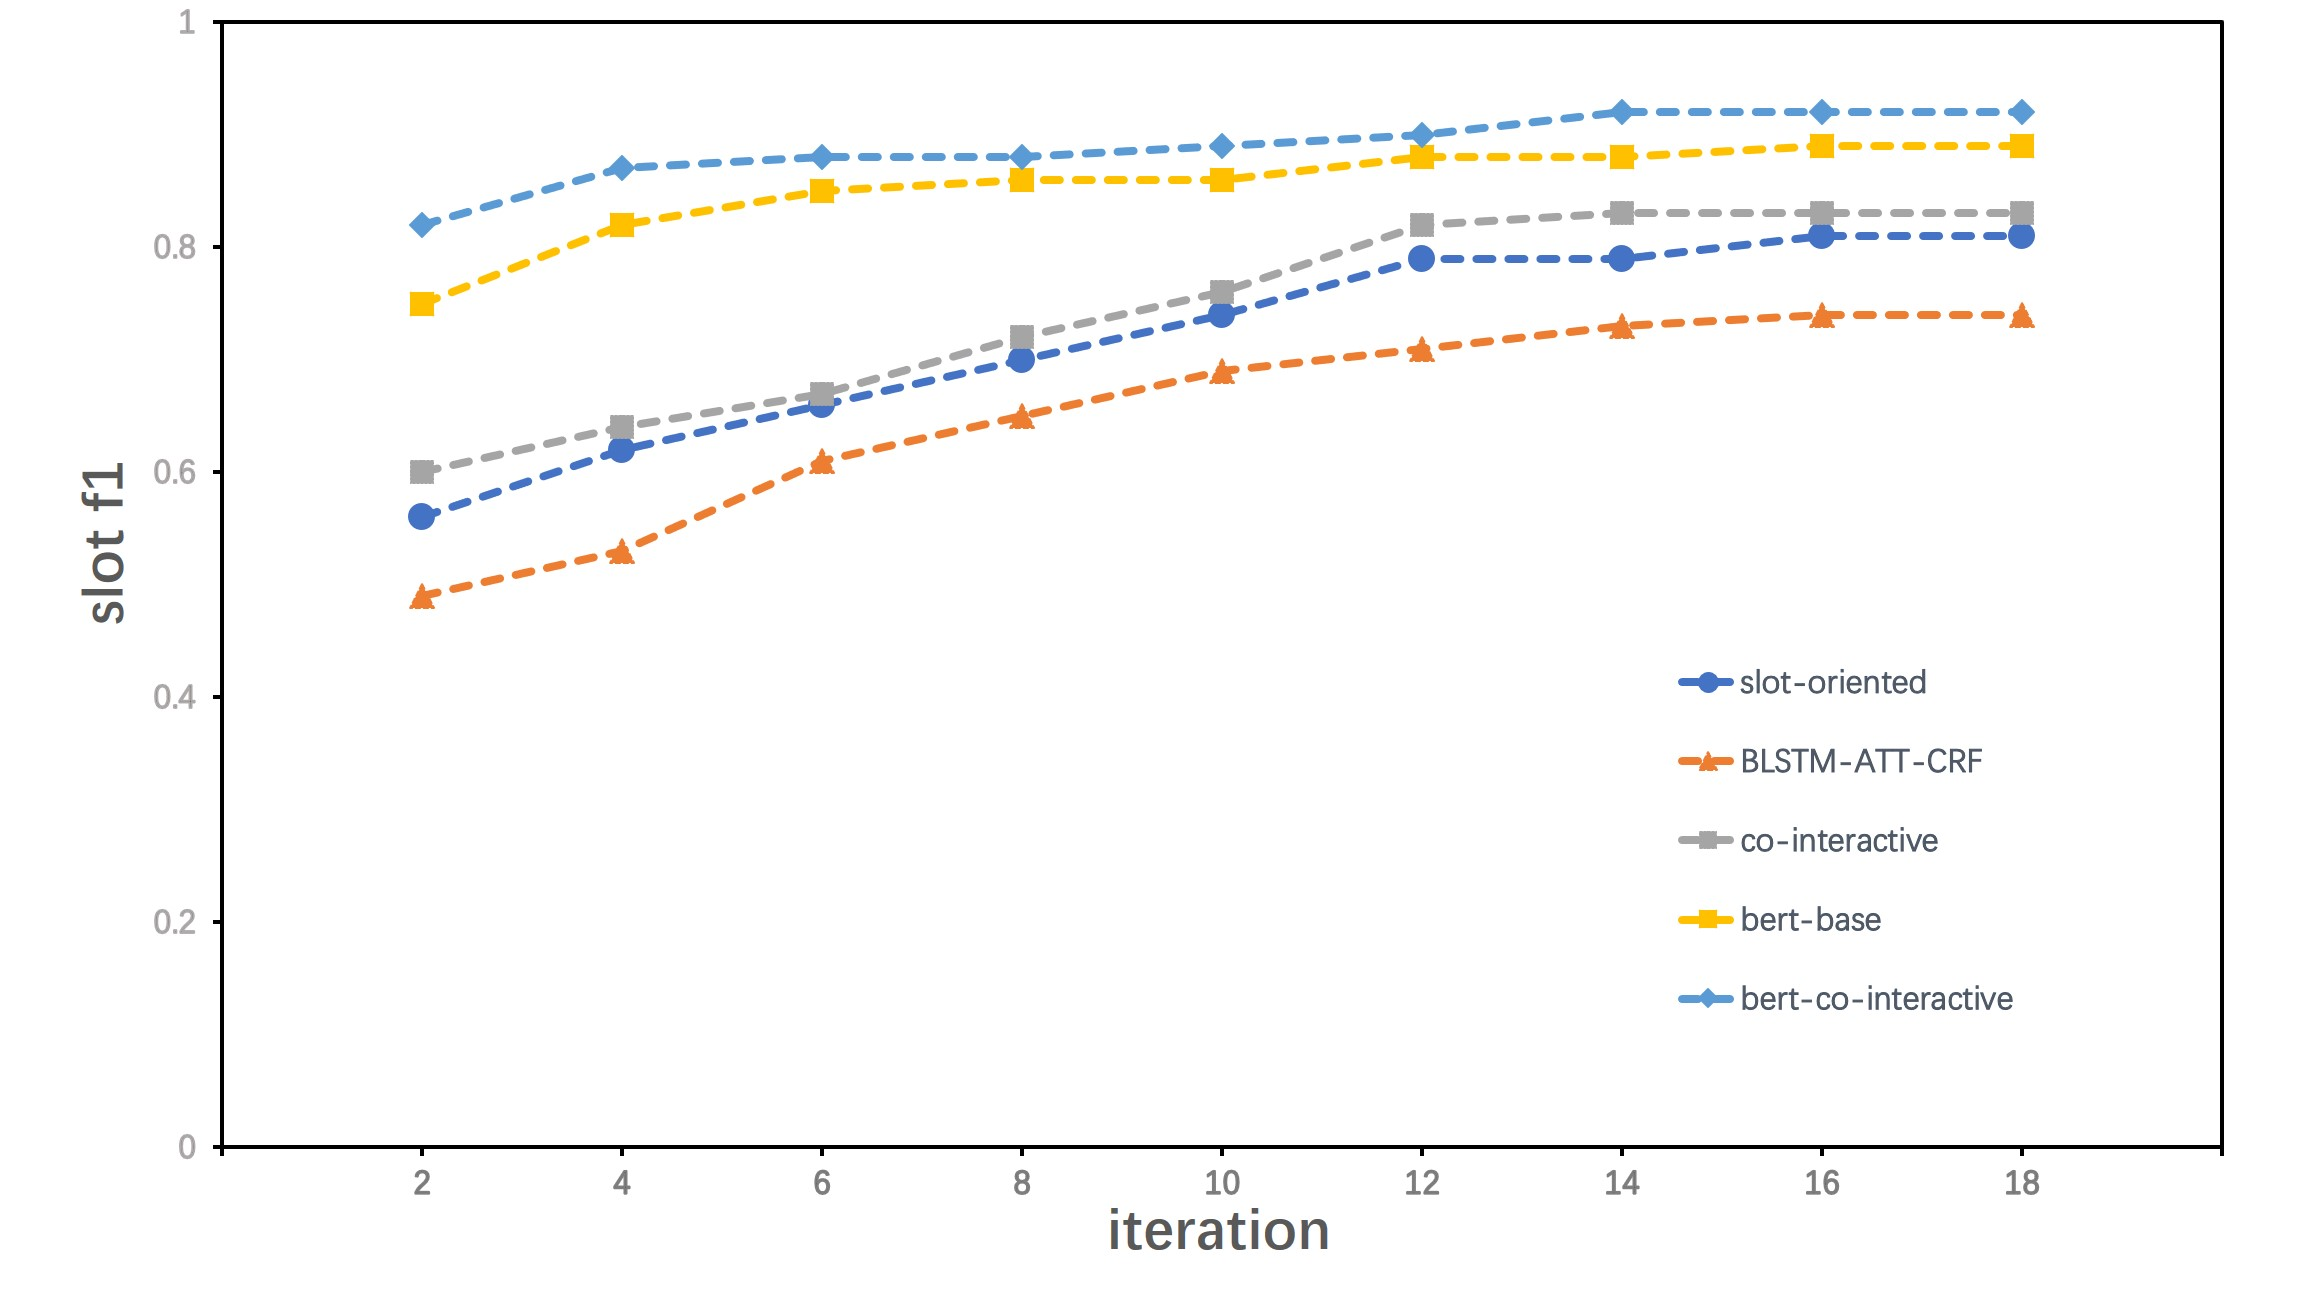
\includegraphics[width=8cm]{./images/slotF1.jpg}
  \label{fig:slotF1}
  }
  % \hspace{5pt}
  %  \hspace{+5mm}
  \subfloat[句子整体的accuracy曲线]{
  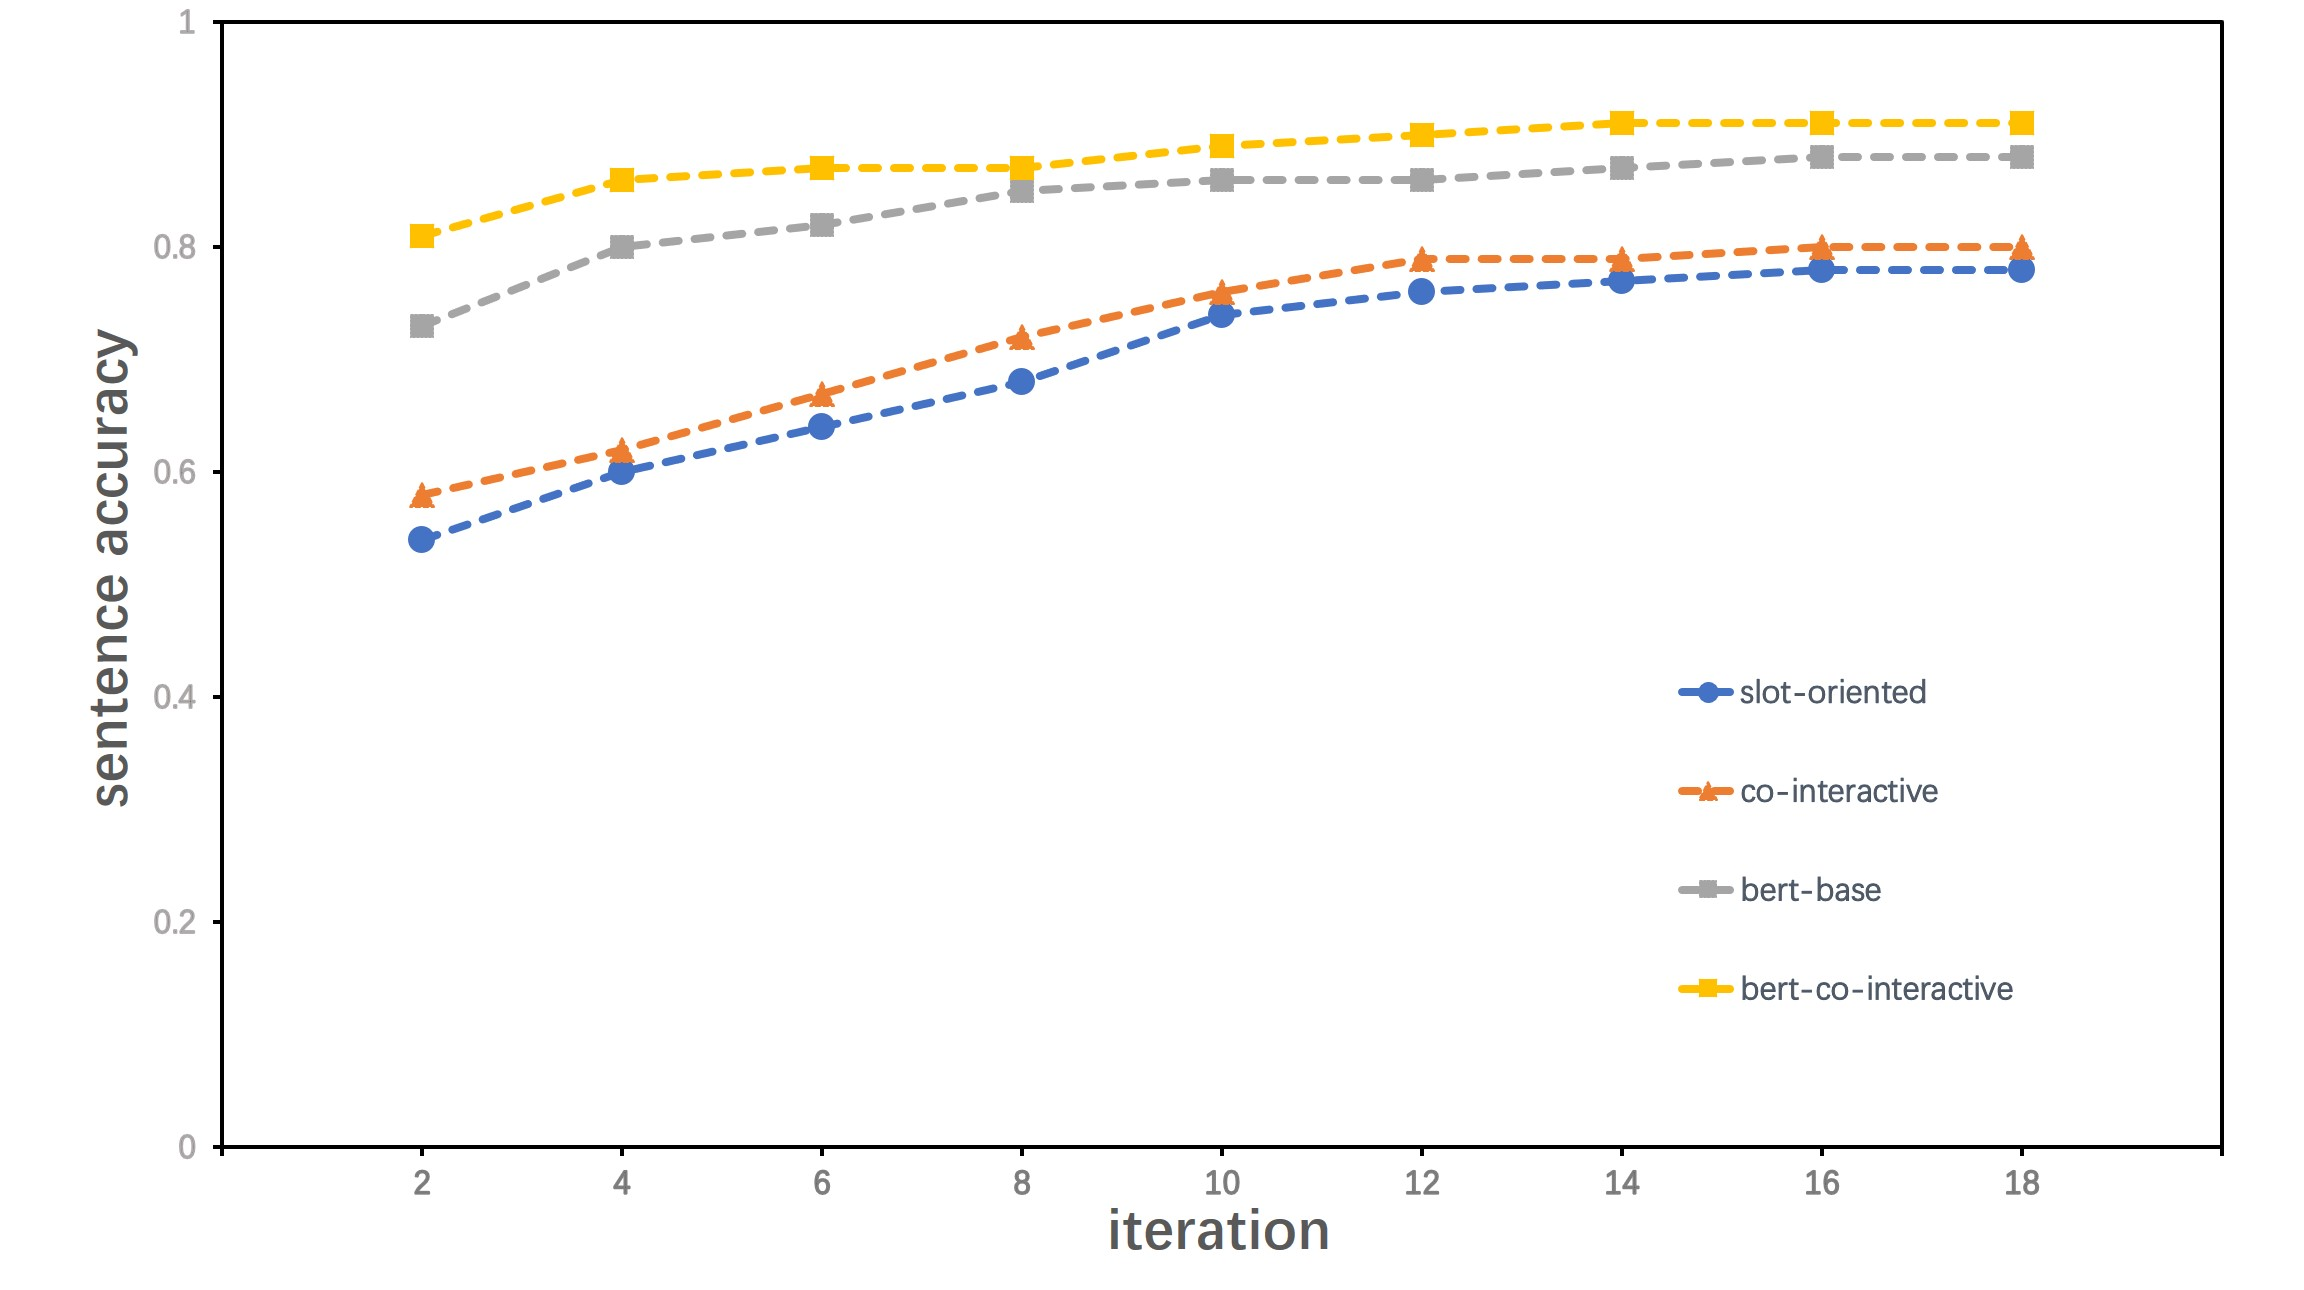
\includegraphics[width=8cm]{./images/sentenceAccuracy.jpg}
  \label{fig:sentenceAccuracy}
  }
  \caption{训练集上各模型指标值的变化}
  \label{fig:4}
  \end{figure}

  实验训练过程中模型的accuracy指标以及$F_1$指标变化如图\ref{fig:4}所示,从图\ref{fig:serviceAccuracy},\ref{fig:interfaceAccuracy}
  可以看到slot-oriented联合识别模型在服务分类和接口分类
  任务中表现不佳,不及ATT-CLSTM模型和Trans-CLSTM模型,原因是slot-oriented模型中信息流是从服务分类
  和接口分类传入语义槽填充,单向的流动并不能对信息源的任务带来增益。虽然如此,图\ref{fig:slotF1}显示,slot-oriented模型在语义槽填充任务上的表现
  优于BiLSTM-attention-CRF,原因在于得到了前两个任务的语义信息补充获得增益。

  预训练模型bert的引入为各项任务的性能带来了显著的提升,一方面,结合预训练的模型在经过较少轮的迭代就可以趋于收敛;
  另一方面,模型最终的指标得分也因为bert的引入而提高。这是由于bert的参数在预训练过程中使用了数据量庞大的语料,
  具有了对许多中文语句很好的理解和编码能力,同时本文的数据集中语料数量有限,导致其他模型不能最大程度的收敛,最终如图\ref{fig:sentenceAccuracy}显示
  结合预训练bert的模型在句子整体的准确率也是最优。

  \begin{table}[htb]
    \centering
    \caption{实验结果表}
    \label{tab:jieguo}
\begin{tabular}{l|cccc}
  \toprule
  \multicolumn{1}{c|}{\centering model}&Service Acc&Interface Acc&Slot $F_1$&Sentence Acc\\
   \hline
   ATT-CLSTM&84.37\%&-&-&-\\
   Trans-CLSTM&-&82.65\%&-&-\\
   BLSTM-ATT-CRF&-&-&74.19\%&-\\
   Slot-oriented&82.13\%&82.09\%&81.83\%&78.31\%\\
   Co-interactive&86.54\%&85.53\%&83.62\%&80.13\%\\
   BERT-base&93.72\%&91.26\%&88.01\%&87.63\%\\
   BERT-co-interactive&$\mathbf{95.18\%}$&$\mathbf{94.91}\%$&$\mathbf{92.23}\%$&$\mathbf{91.47}\%$\\
  \bottomrule
  \end{tabular}
\end{table}

本文所有模型的实验结果如表\ref{tab:jieguo}所示,以下是对结果数据的展开分析。
在多个任务中,对比结合预训练的模型和传统深度学习模型,“bert+”模式的结构对性能有很大的提升,这也证明了bert在语义理解任务中的作用和重要意义。
传统的深度学习方法不及“bert+”模式的原因在于训练的数据集有限,模型训练不充分,导致泛化能力较弱,而bert已在大规模语料训练中对下游任务有了初步的建模。

对于服务分类、接口分类和参数提取(语义槽填充)这三项强相关的任务,从其他任务中获得决策信息对当前任务的预测大有裨益,实验结果也验证了这一猜想,
slot-oriented联合识别模型由于获得了服务类别和接口类别信息,在参数提取(语义槽填充)任务上的$F_1$值相较于BiLSTM-attention-CRF有所提升,前两项任务表现
不佳是由于服务和接口的分类预测时并没有获得其他任务的决策信息增益,相反的,单向联合在前两项任务中设计的十分简单,
co-interactive联合识别模型则在三项任务中都有超过传统深度学习模型的表现。
\begin{table}[htb]
  \centering
  \caption{消融分析}
  \label{tab:xiaorongjieguo}
\begin{tabular}{l|cccc}
  \toprule
  \multicolumn{1}{c|}{\centering model}&Service Acc&Interface Acc&Slot $F_1$&Sentence Acc\\
 \hline
 删除bert&86.54\%&85.53\%&83.62\%&80.13\%\\
 删除service attention层&94.55\%&94.52\%&92.01\%&91.03\%\\
 删除interface attention层&95.02\%&93.51\%&91.99\%&91.12\%\\
 删除slot attention层&94.98\%&94.47\%&91.13\%&90.27\%\\
 (service,interface)-to-slot&93.47\%&93.85\%&91.99\%&90.46\%\\
 (service,slot)-to-interface&93.52\%&93.77\%&91.08\%&90.31\%\\
 (interface,slot)-to-service&94.53\%&93.81\%&91.12\%&90.02\%\\
 bert-co-interactive&$\mathbf{95.18\%}$&$\mathbf{94.91}\%$&$\mathbf{92.23}\%$&$\mathbf{91.47}\%$\\
\bottomrule
\end{tabular}
\end{table}
从bert-base和bert-co-interactive联合识别两组模型的对比中可以看出,相较于基础的softmax分类,在预训练模型上增加针对于语义理解的特定结构,模型效果会有所提升。
其中语义槽填充任务效果提升最为明显,原因是该任务相比于分类更为复杂,要求模型对语义理解的精度更高,因此模型之间在此任务之上表现的区分度很高。

\begin{figure}[htbp]
  % \centering
  % \hspace{-7mm}
  \subfloat[服务Service分类的accuracy曲线]{
  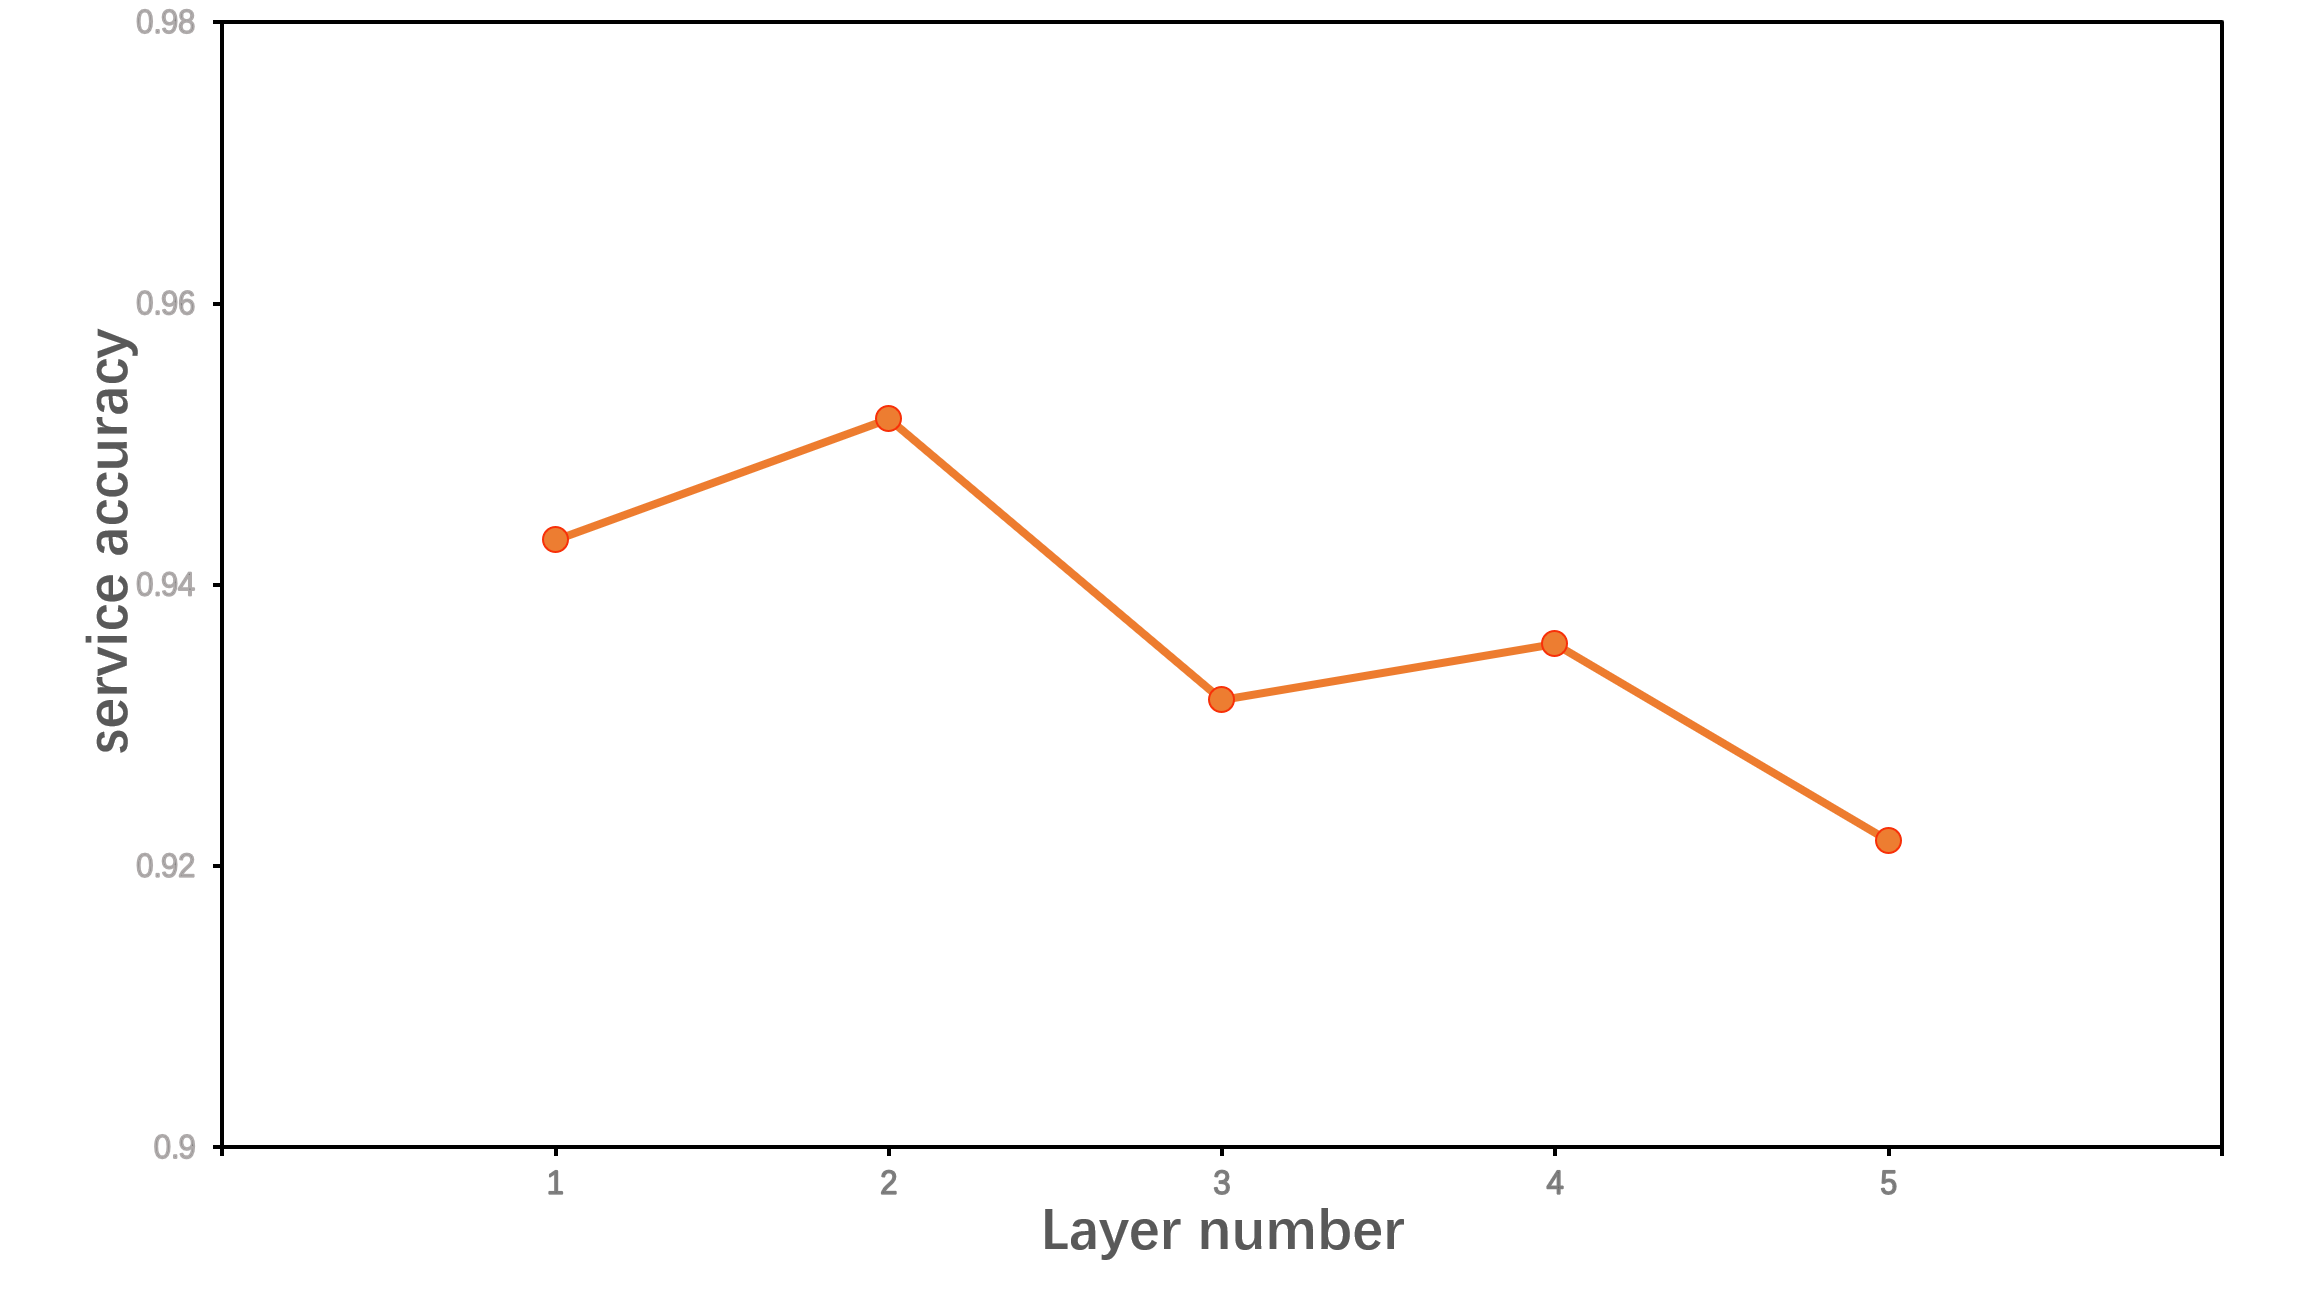
\includegraphics[width=8cm]{./images/layerService.png}
  \label{fig:serviceAccuracy2}
  }
  % \hspace{5pt}
    % \hspace{+5mm}
  \subfloat[接口Interface分类的accuracy曲线]{
  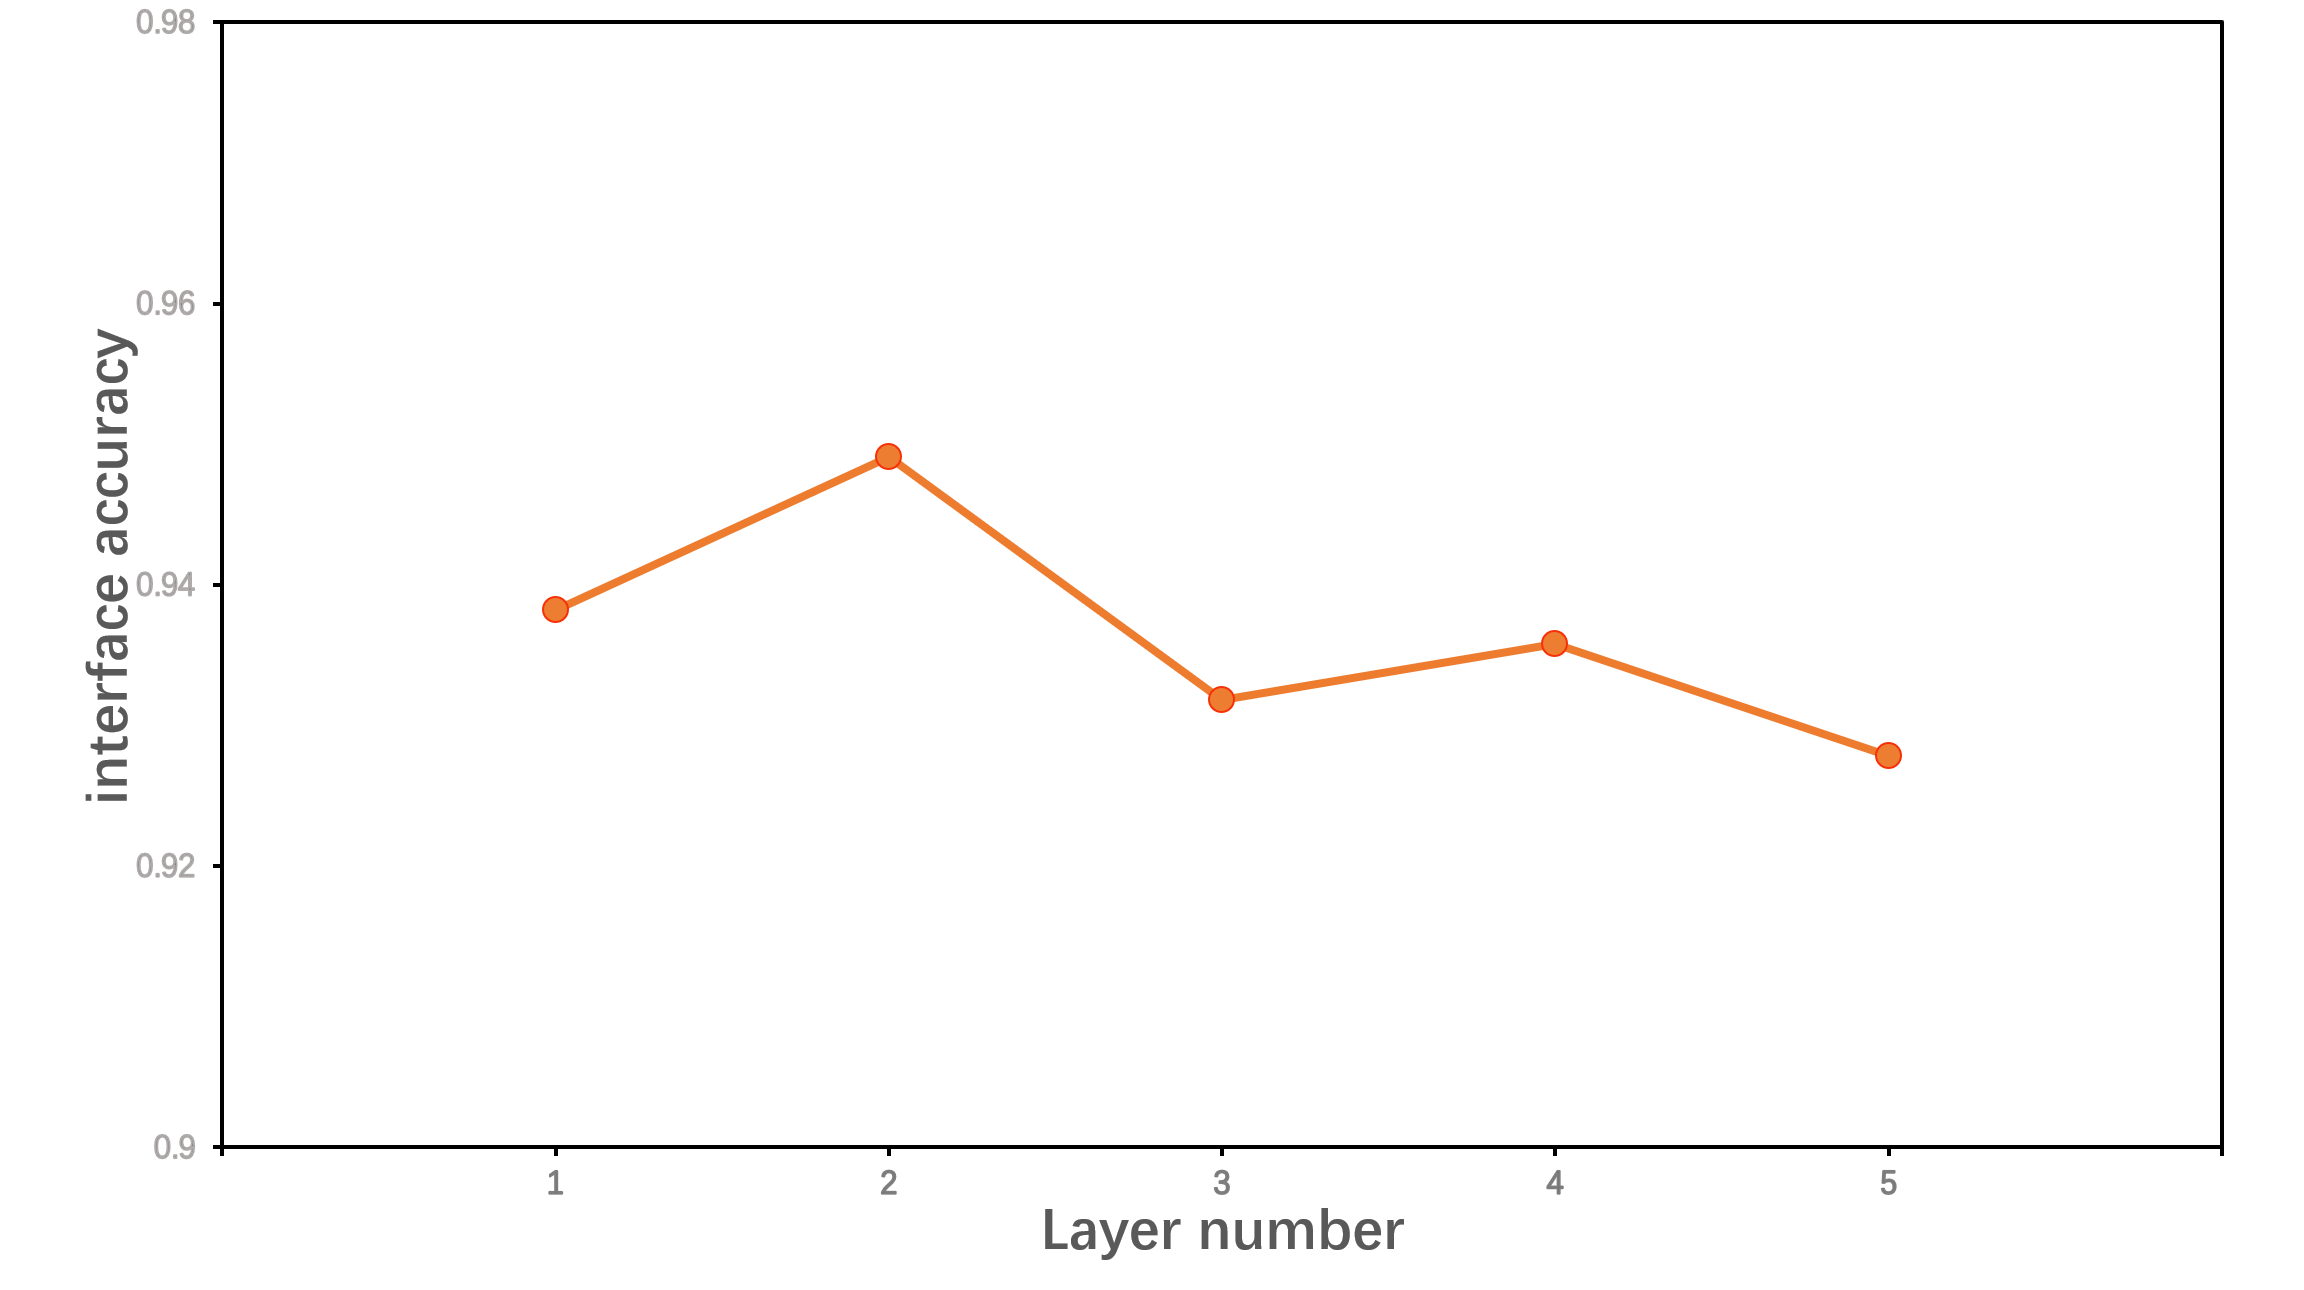
\includegraphics[width=8cm]{./images/layerInterface.png}
  \label{fig:interfaceAccuracy2}
  }\\
  % \hspace{5pt}
  %  \hspace{-7mm}
  \subfloat[语义槽填充的$F_1$曲线]{
  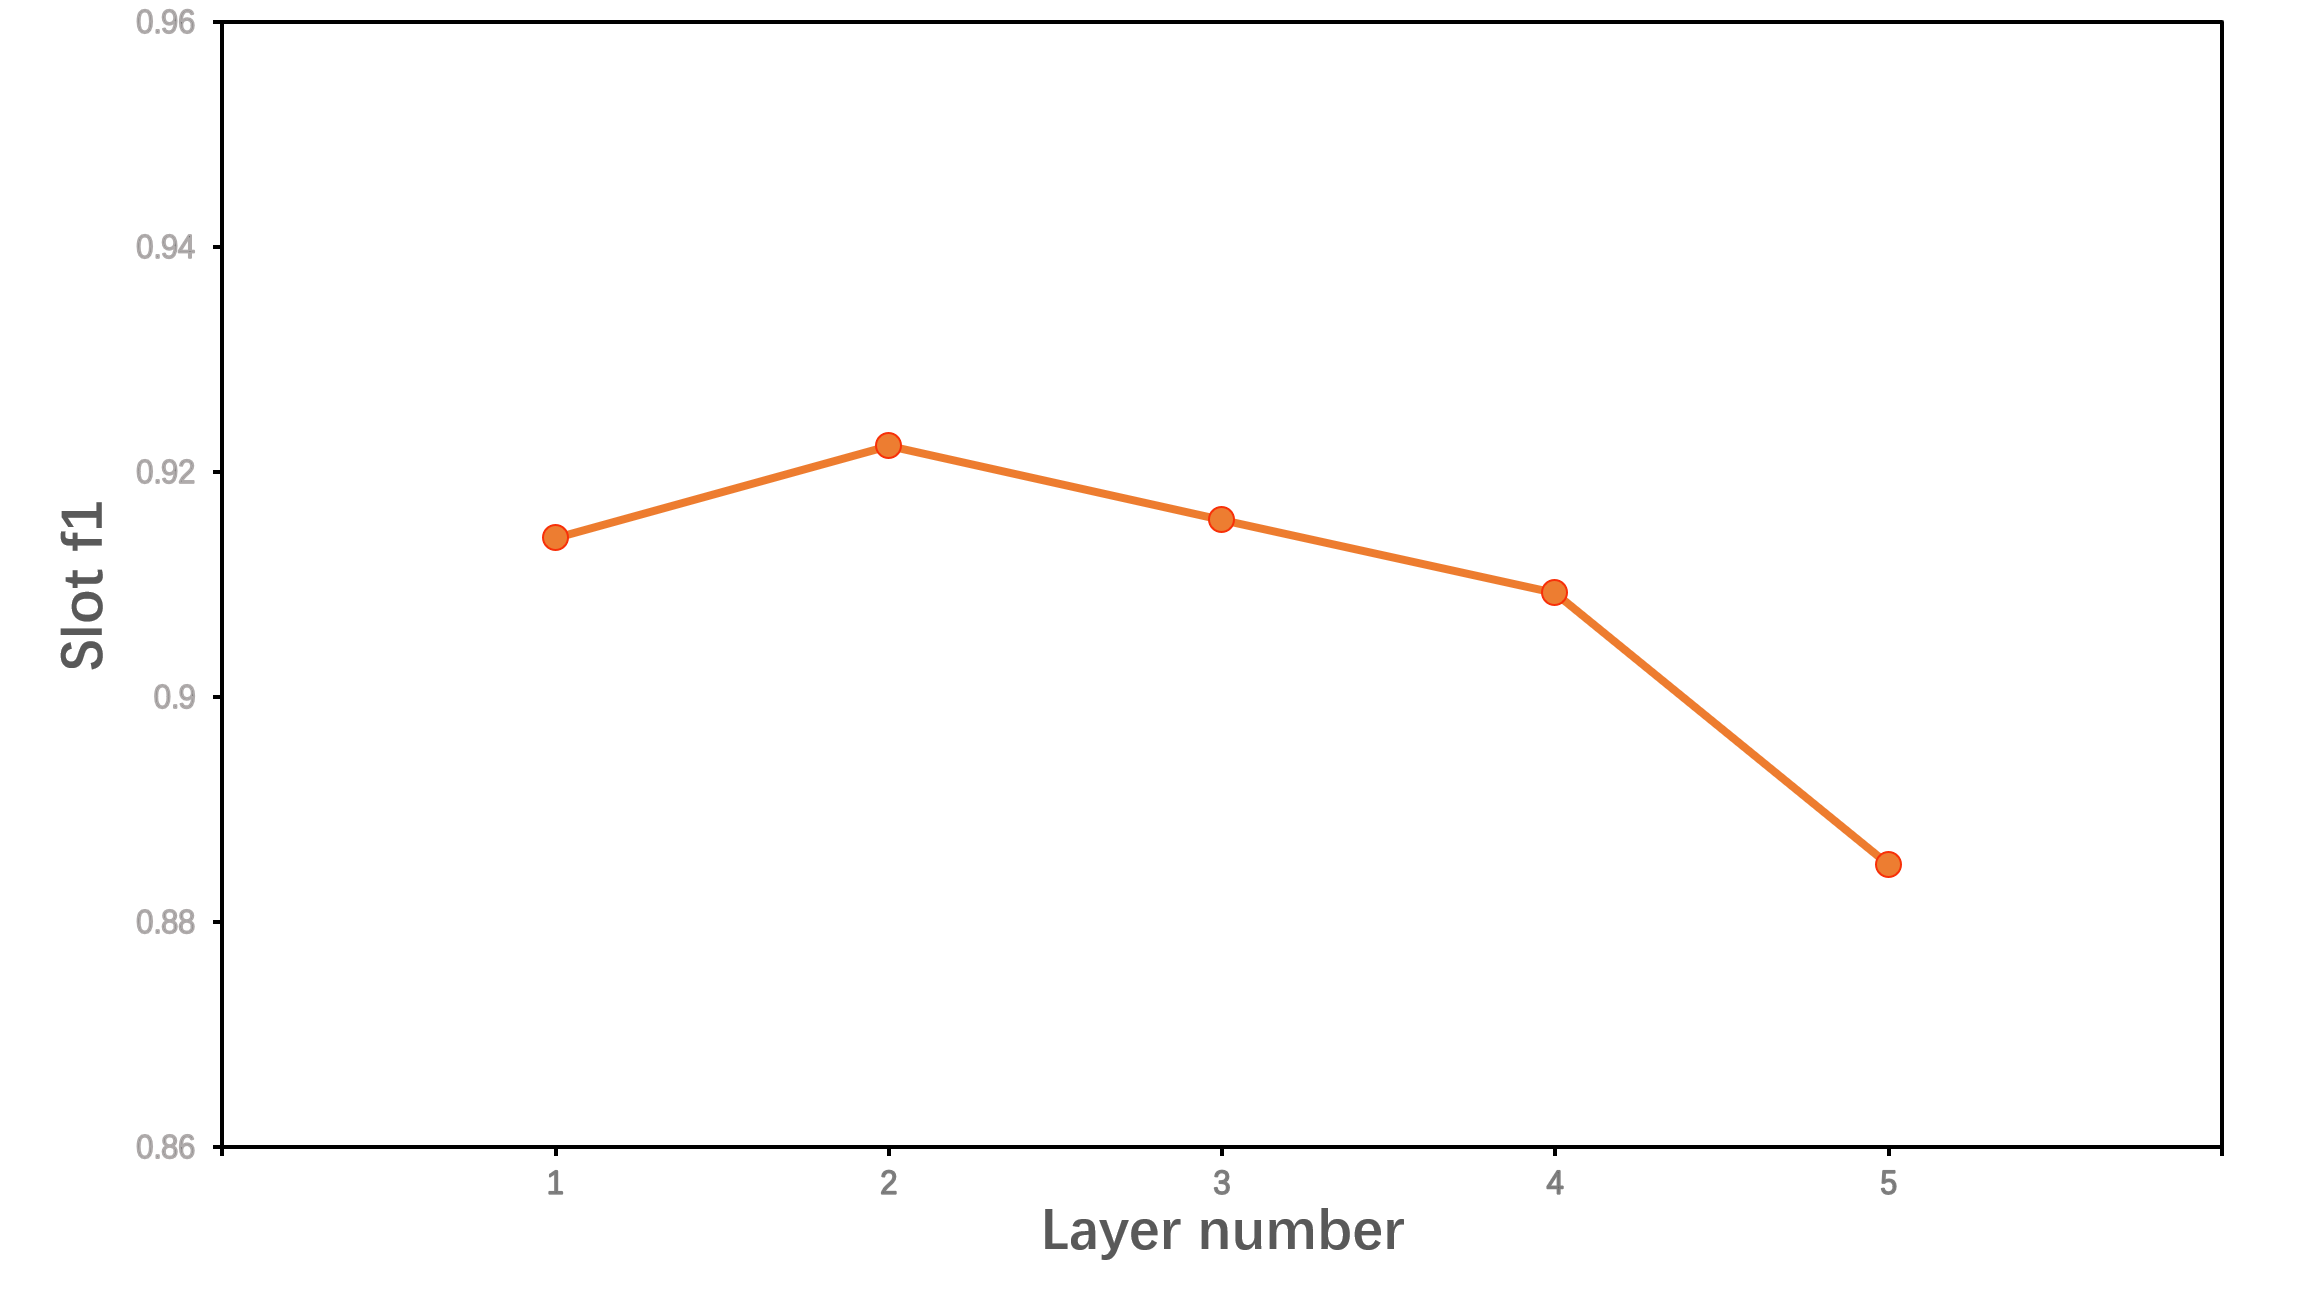
\includegraphics[width=8cm]{./images/layerSlot.png}
  \label{fig:slotF12}
  }
  % \hspace{5pt}
  %  \hspace{+5mm}
  \subfloat[句子整体的accuracy曲线]{
  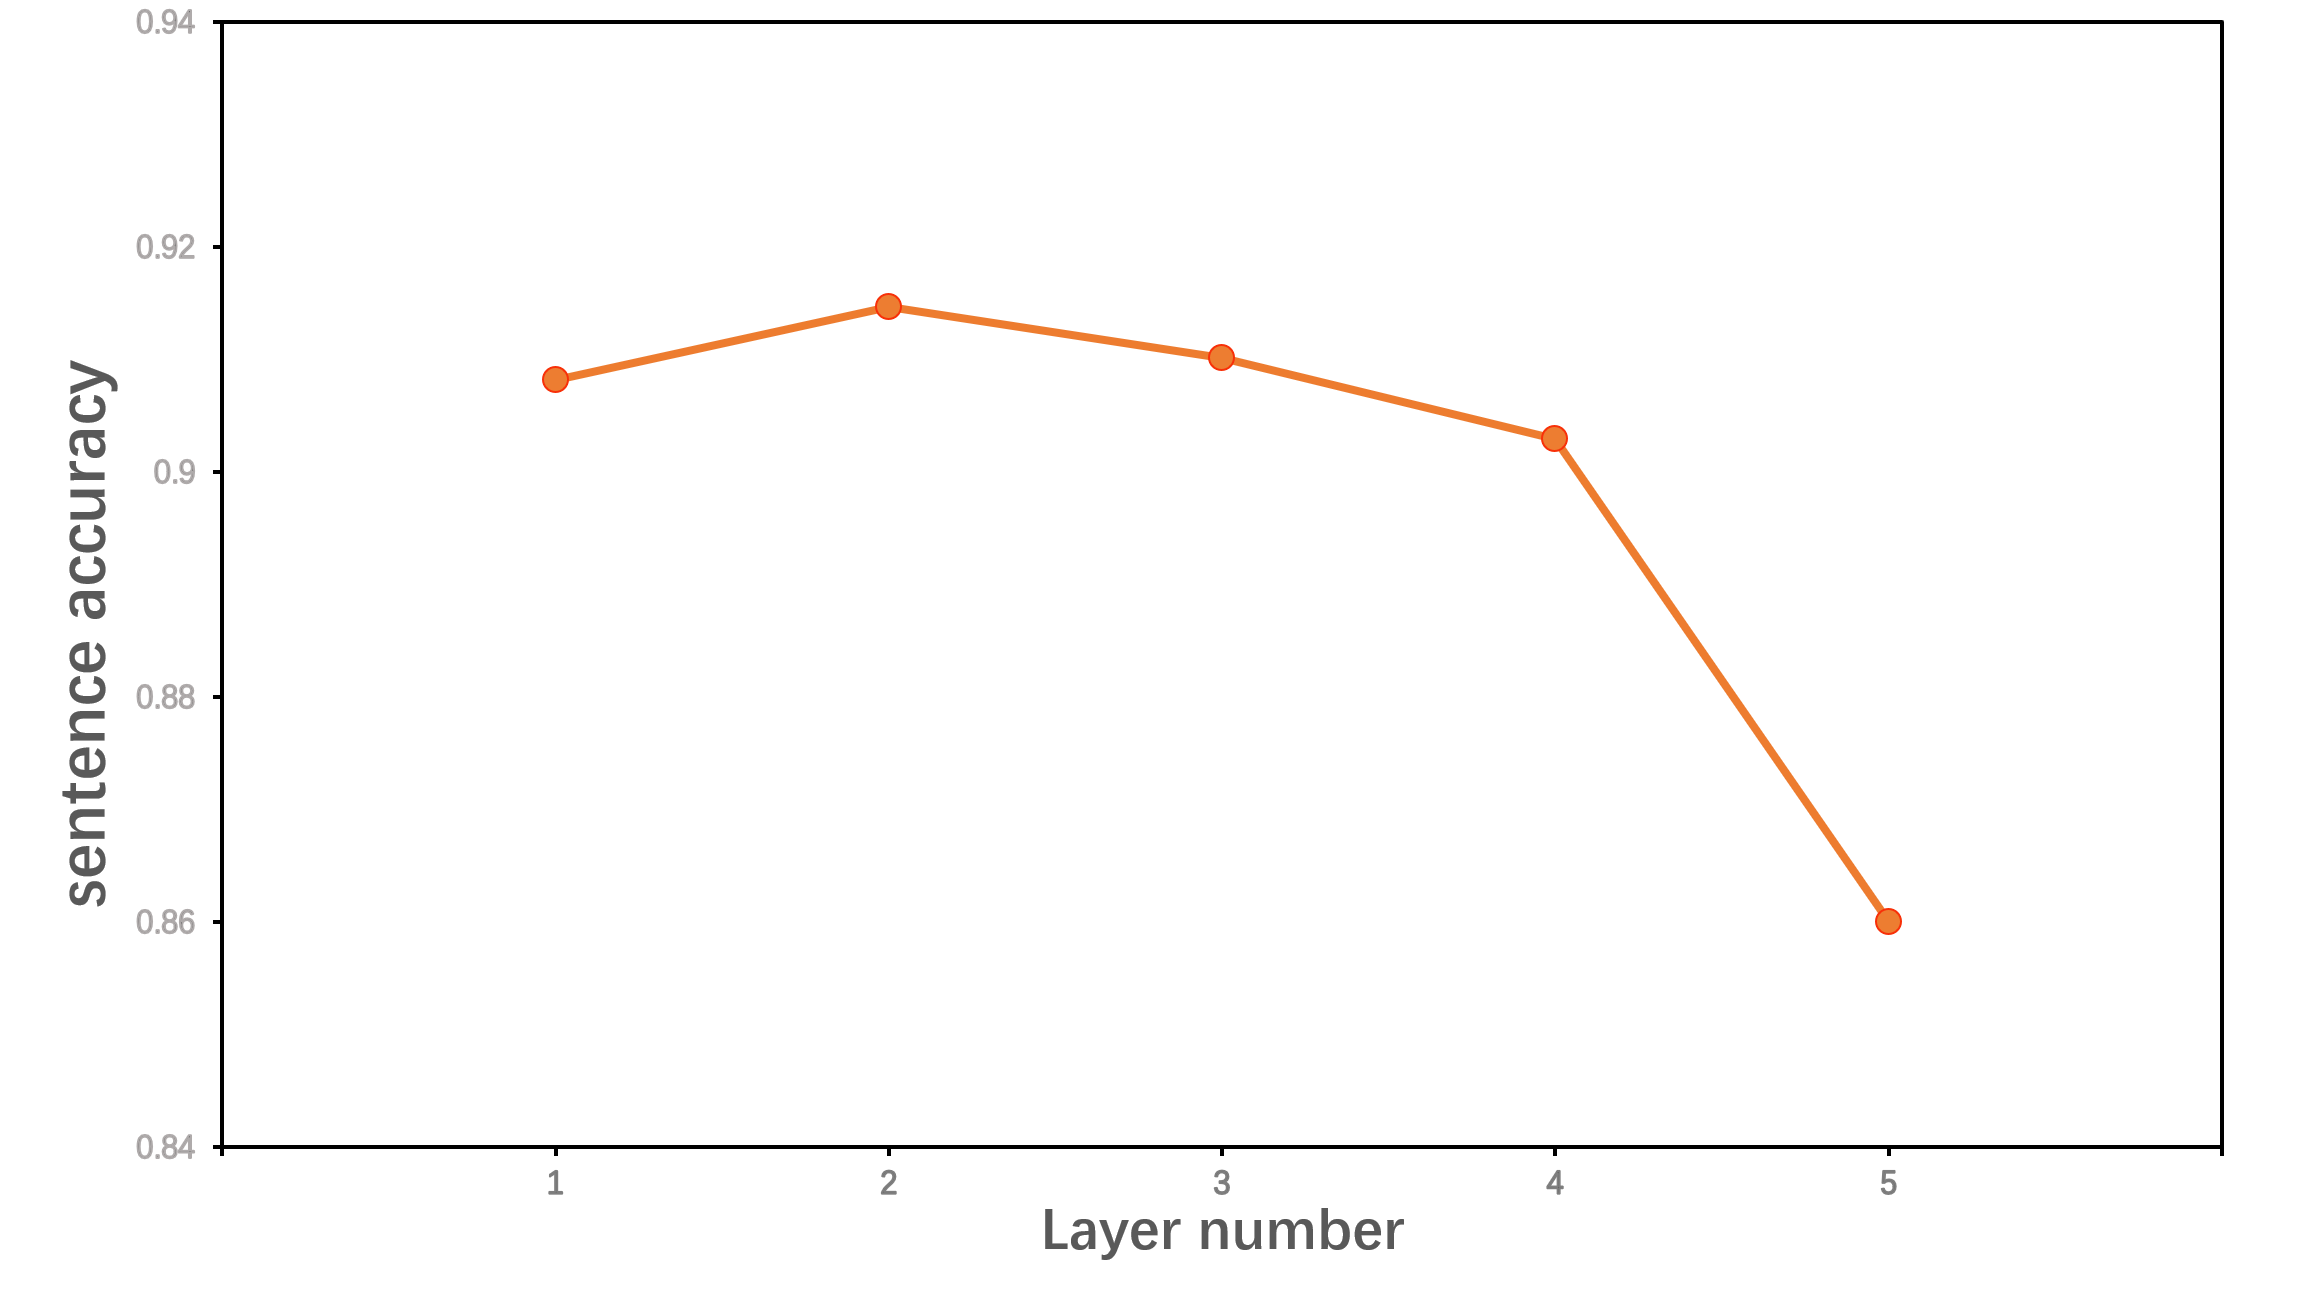
\includegraphics[width=8cm]{./images/layerSentence.png}
  \label{fig:sentenceAccuracy2}
  }
  \caption{bert-co-interactive不同堆叠层数模型性能比较}
  \label{fig:layerCompare}
  \end{figure}
对于测试集表现最优的bert-co-interactive联合识别模型,我们进行了进一步消融分析。消融分析直白的解释就是将模型视作pipeline,在模型整体性能较好的前提下,
我们希望分析出pipeline中结构A,B,C等对性能的影响,逐个剔除A,B,C做控制变量法的对比实验,探索模型中各模块对性能的影响和贡献,
消融分析实验结果如表\ref{tab:xiaorongjieguo}所示。

首先bert预训练层的移除对实验结果影响巨大,各指标断崖式下跌,可见bert的引入对结果至关重要。
之后我们分别剔除了service attention层,interface attention层和slot attention层,将共享编码层的输出$\mathbf{H}$=[$h_{1}$,$h_{2}$,\dots,$h_{n}$]直接
输入到交互层,三次实验结果显示,分类的准确率以及语义槽$F_1$值均有所下降,表明对编码层向量做初步的attention处理增强语义表示,对于多个任务之间的协同交互有帮助。
然后我们修改了交互层的结构,由原来的信息多向交互共享转为单向的信息传递,三次实验分别是服务、接口信息流向语义槽填充任务((service,interface)-to-slot),
接口、语义槽填充信息流向服务分类任务((interface,slot)-to-service),服务、语义槽填充信息流向接口分类任务((service,slot)-to-interface),我们
只保留了信息的单向流通,实验结果显示单向的信息流动相比于交互式的互相增强,会对准确率造成影响,均有所下降,这表明
对服务分类、接口分类和参数提取(语义槽填充)之间的交互建模可以以一种相互增强的方式来增强这三项任务。相反,如果仅考虑信息流的单个方向作用,而忽略另一个任务信息
的反哺能力,则不能带到更优的结果。


对于bert-co-interactive联合识别模型,我们也探讨了协同交互模块的堆叠层数量对性能的影响,对比实验如图\ref{fig:layerCompare}所示。
可以看到,N的值从1增加到2时各指标均有所提升,说明使用一定深度的层次堆叠可以带来更好的性能,
这是因为协同交互模块堆叠在一起形成层次结构,使任务之间能够进行多次交互,从而实现增量捕获交互信息来达到彼此丰富,
进而更好地为任务之间交互建模,并学习相互间的知识。 
但是当堆叠的层数超过三层时,模型性能会变差,
这其中的原因可能是随着整个网络的深入,出现梯度消失或过度拟合问题。
最终模型超参数N被定为2。

  为了更好地了解模型学到了什么,让模型的设计更具可解释性,我们将co-interactive联合识别模型的协同交互层中部分矩阵做了可视化处理\ref{fig:visual}。
  对于参数提取(语义槽填充)任务,在co-interactive联合识别模型的协同交互层中进行信息交互时,主要做了
  将参数填充向量视为查询$Q_S$,服务分类向量视为键$K_D$以及值$V_D$,以获取可感知参数填充信息的服务分类向量表示信息并反馈给参数填充任务;
接口分类向量视为键$K_I$以及值$V_I$,以获取可感知参数填充信息的接口向量表示信息并反馈给参数填充任务。
  为此,我们将$Q_S$,$K_D$,$V_D$计算后的矩阵可视化,它表示了服务分类向量指导下各语义槽受到的注意力分布,
  从图中可以观察到:(1)我们的模型在服务类别向量$K_D$(包含有train的语义)指导下将注意权重集中在正确的语义槽(“成都”和“杭州”)上,
  这表明协同交互层任务间注意力机制可以指导模型学习。
  (2)使用更深的层(第二层\ref{fig:77777})可以更好地帮助模型捕获相关的语义槽,与第一层\ref{fig:777}相比,注意力着色更暗(表明得分高),
  这是因为协同交互模块堆叠在一起形成层次结构,使任务之间能够进行多次交互,从而实现增量捕获交互信息来达到彼此丰富。

  \begin{table}[htb]
    \centering
    \caption{引入知识库实验结果表}
    \label{tab:kbjieguo}
\begin{tabular}{l|cccc}
  \toprule
  \multicolumn{1}{c|}{\centering model}&Service Acc&Interface Acc&Slot $F_1$&Sentence Acc\\
   \hline
   BERT-co-interactive&$95.18\%$&$94.91\%$&$92.23\%$&$91.47\%$\\
   BERT-kb-co-interactive&$\mathbf{95.31\%}$&$\mathbf{95.22}\%$&$\mathbf{94.01}\%$&$\mathbf{92.03}\%$\\
   删除C-T attention&$95.22\%$&$94.95\%$&$92.86\%$&$91.53\%$\\
  \bottomrule
  \end{tabular}
\end{table}

\begin{figure}[htbp]
  \centering
 % \hspace{-7mm}
 \subfloat[第一层]{
 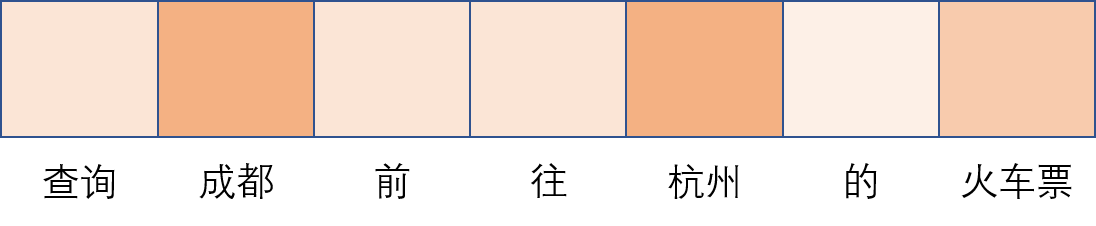
\includegraphics[width=8cm]{./images/first.png}
 \label{fig:777}
 }
 % \hspace{5pt}
   % \hspace{+5mm}
   \centering
 \subfloat[第二层]{
 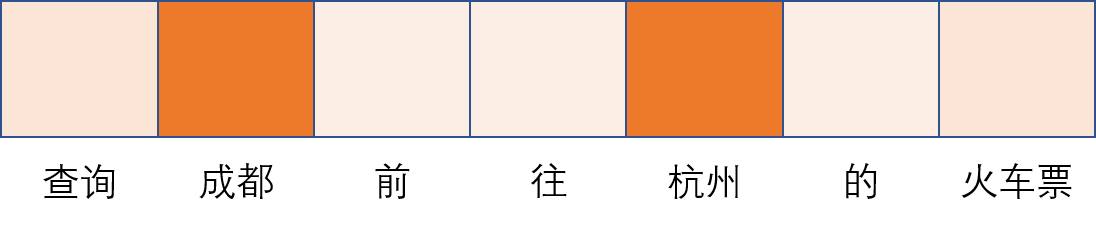
\includegraphics[width=8cm]{./images/second.png}
 \label{fig:77777}
 }
 \caption{协同交互层slot向量可视化}
 \label{fig:visual}
 \end{figure}
最后,我们对BERT-co-interactive编码层做了改进,引入了知识图谱,对比实验结果如表\ref{tab:kbjieguo}所示,
可以发现,知识库的引入能够给模型性能带来提升。短文本输入做为信息源相对较模糊,它没有足够的上下文信息,
从外部知识源中检索知识,将概念性信息视为一种知识传入神经网络,可以增强短文本的语义表示。
模型编码层借助知识库(KB)丰富了短文本的信息,将知识库中的先验知识作为显式特征纳入DNN中,这对短文本分类有很大贡献。
与传统的DNN相比,引入知识模型能够基于观察力(机器的训练数据)和现有知识做出决策。
如表中第三行所示,我们对BERT-kb-co-interactive中C-T attention模块做了消融实验,发现删除C-T attention模块后实验指标有所下降,
这是因为失去C-T attention模块的模型在引入知识概念是不会考虑概念是否与文本相关,很可能会带来不相关的概率从而造成数据噪声影响了模型的判断。
如图\ref{fig:ctattention}所示,以文本“播放林俊杰的江南”为例,我们将C-T attention模块的权值进行了可视化,
可以看到模型成功将注意力集中在歌手和歌名上,避开了噪声概念,这正是引入C-T attention的初衷。
此外,由于注意力机制,我们的模型能够更加关注重要的知识
但是四项指标的提升并不明显,可能是因为测试集数量有限,其中并没有太多需要引入外部知识的测试样例。
\begin{figure}[htbp]
  \centering
  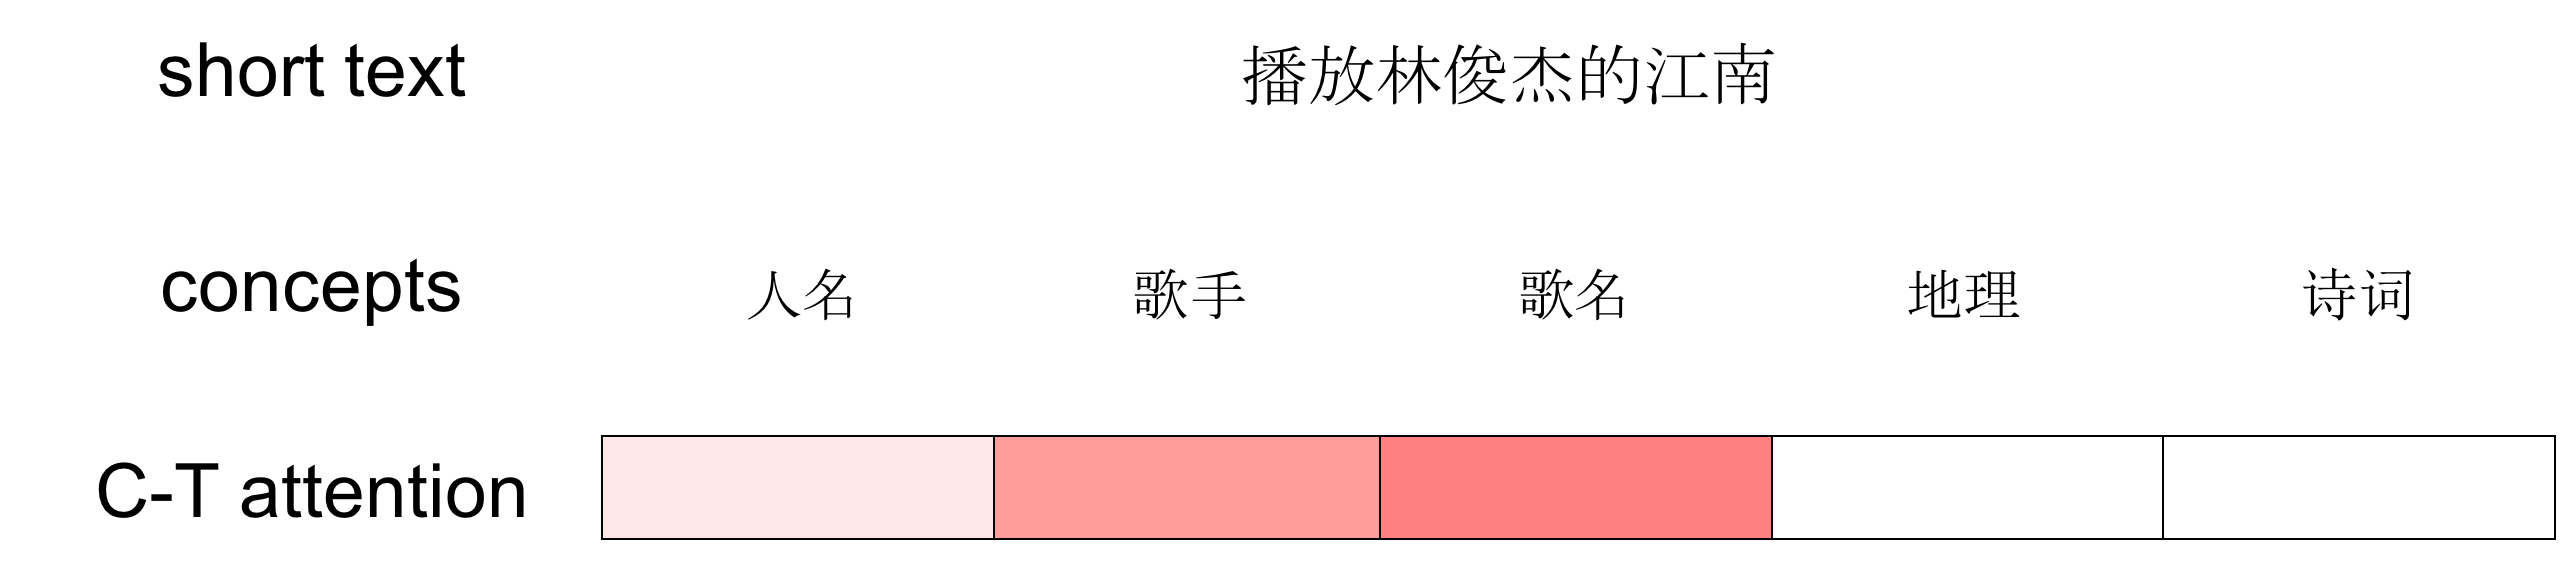
\includegraphics[scale=0.3]{./images/ctattention.png}
  \caption{C-T attention权值可视化}
  \label{fig:ctattention}
\end{figure}

  \section{本章小结}
  本章介绍了跨界服务领域数据集的构建,对数据集的预处理划分和实验结果的评价指标,
对前两章提出的模型进行了实验,其中进行了多组对照得出bert-co-interactive具有更好的性能,同时对bert-co-interactive
做了消融实验分析各结构对性能的影响。

\chapter{系统设计与架构}
本文在之前已详细介绍了用户语义理解模型的算法部分,为将算法与应用相结合,利用现有的跨界服务
网络系统JTangYdrail,设计了服务智能调用引擎的系统架构。本章将相对跨界服务
网络系统架构做简要介绍,之后展开讨论与语义理解相关的系统模块。

\section{跨界服务网络系统}
本文作者所在的课题组系统性地研究了跨界服务相关理论,并形成了跨界服务原型系统,
本节主要介绍系统整体架构以及跨界服务系统中两个核心模块服务交换机和服务路由器\cite{zheng2020service}。

  跨界服务系统是针对跨界服务运行时呈现高维异构、复杂动态、开放分布的特点,解决跨界服务网络管理中高效接入、安
  全交换、智能路由等关键技术,形成的跨界服务集成工程化方法,研制软硬件结合的跨
  界服务集成及运行支撑载体,包括跨界服务集成设计软件套件、服务交换机与路由器硬
  件环境。

  海量跨界服务分布于服务网络中,不同服务之间相互操作,通过服务交换及路由技术,实现跨界服务的查找、调用
  及跨界服务间的交互,同时利用基于认证授权的开放服务安全交换技术,保证交换
  过程中的数据安全。服务交换机和服务路由器是支撑载体的关键,采用软硬结合
  的设计方案来实现,如图\ref{fig:system}所示,服务交换机实现跨界服务的高效接入、访问控制、消
  息映射、认证授权等功能,实现域内企业服务的安全可靠的开放,其架构包括设施层(机
  柜、电源、接口等)、设备层(计算服务器、存储服务器)、网络层(虚拟路由器、虚拟
  防火墙)、应用层(服务接入、访问控制、服务缓存等)\cite{刘皇敏2019跨界服务网络关键技术研究}。服务路由器提供服务聚合、
  服务查找、服务路由等能力,把异构服务联成网络,是跨界服务互联的基础设施,其架
  构包括设施层(机柜、电源、接口等)、设备层(计算服务器、存储服务器)、网络层(状
  态感知、消息路由等功能)、应用层(服务索引、服务查找、服务路由等)。

  \begin{figure}[htbp]
    \centering
    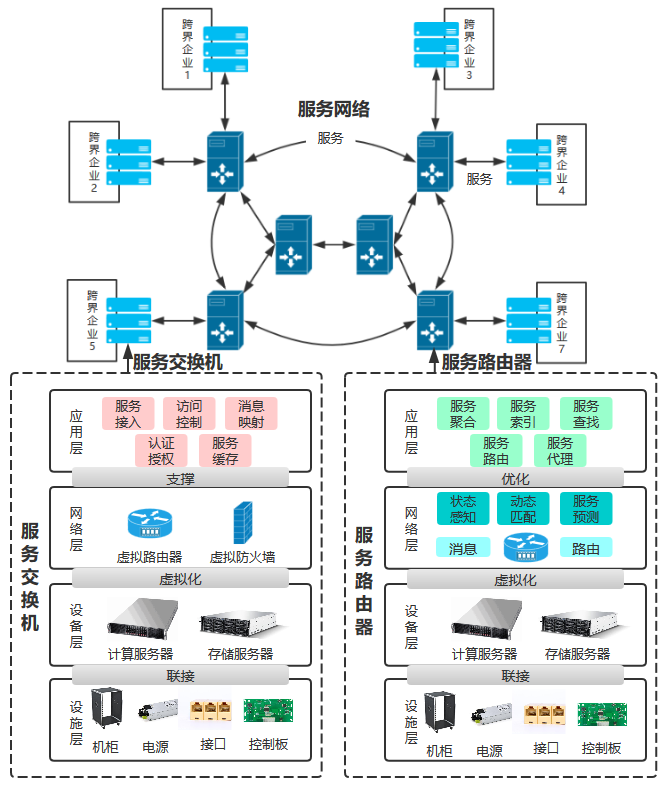
\includegraphics[width=10cm]{./images/system.png}
    \caption{JTangYdrail系统架构\cite{zhanghuan}}
    \label{fig:system}
  \end{figure}

  服务交换机是跨界服务网络上最下层节点,
  使用服务地址在交换层接收并转发服务相关的数据,与实际服务直接相关,
  是服务的拥有者以及一次服务远程调用的发起者。
    服务路由器是在服务网络中转发服务元信息的网络设备,一方面,服务路由器从服务交换机收集服务信息,并在整个网络中广播数据。 
    另一方面,如果用户调用服务,则服务路由器会将请求转发到相应的服务节点。 
    % 如图\ref{fig:switchboard}所示,主要包含以下几个模块:

% 1)注册模块:维护企业的服务信息和业务数据,
% 服务成功注册后,服务信息将存储在本地,并且其元数据将通过泛洪或其他方式广播到整个网络。
% 此后不久,其他服务交换机即可搜索和使用该服务交换机上服务。

% 2)适配器模块:旨在支持环境异构,AdM提供了各种适配器,可以通过不同的语言实现这些适配器,以实现与异构服务的通信。
% 在语义上兼容前提下,尽管硬件和软件平台,语言和API不同,但连接到不同适配器的各种服务在跨界服务系统仍将被连接和集成。

% 3)策略模块:使用多种策略来提高性能,代理策略使用户可以通过代理调用服务,服务交换机的负载平衡策略通过增加进程数来实现可伸缩性和负载平衡,
% 服务缓存策略使某些节点可以缓存服务调用的结果,从而可以充分利用网络中边缘节点的资源。 

% 4)映射模块:旨在为用户带来便利,以特定格式调用服务或接收结果。
%  提供了直观的图形界面,供用户生成规则文件。 
 
% 5)权限模块:是基于密钥加密技术设计的,并使用基于角色的访问控制策略来保护数据的安全性。

  % \begin{figure}[htbp]
  %   \subfloat[JTangYdrail 服务交换机软件架构\cite{zhanghuan}]{
  %     \centering
  %     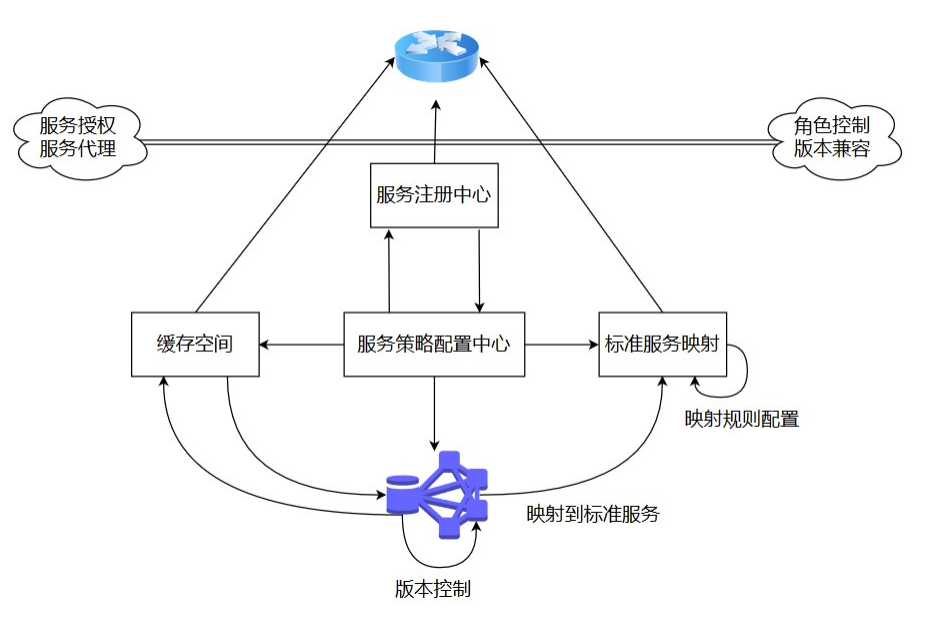
\includegraphics[width=8cm]{./images/switchboard.png}
  %     \label{fig:switchboard}
  %   }
  %   \subfloat[JTangYdrail 服务路由器软件架构\cite{zhanghuan}]{
  %     \centering
  %     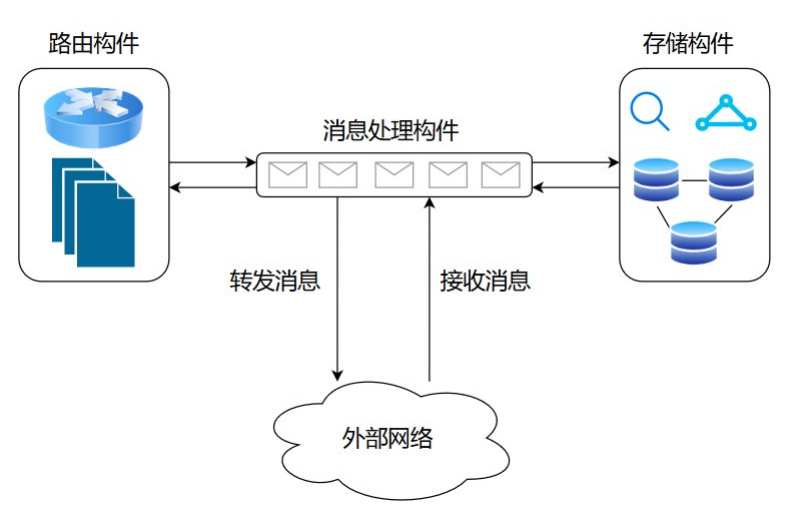
\includegraphics[width=8cm]{./images/router.png}
  %     \label{fig:router}
  %   }
  %   \caption{服务交换机和服务路由器架构}
  %   \label{fig:switchboardAndRouter}
  %   \end{figure}
    
    % 服务路由器的结构如图\ref{fig:router}所示,其中包含路由组件,存储组件,处理器组件等:

    % 1)存储模块:由三部分组成:服务缓存,包括一些服务元数据和一些查询结果;
    % 路由信息,这是整个网络的基础,以及服务网络的结构信息。
    
    % 2)路由模块:功能是根据服务ID转发服务请求,该服务ID与传统网络中的IP地址完全不同。
    
    % 3)处理器模块:提供内部和外部资源之间的通信机制。消息有两种类型:服务消息和路由消息。
    % 一旦收到消息,它将由PrC进行预处理,然后传输到路由组件或存储组件。
    
    % 4)标准服务模块:标准化服务组件设计用于服务网络中功能相似的同类服务,
    % 当发现Web服务的任何故障时,它可以通过使用标准化服务动态地将服务替换为合适的服务,从而大大提高了服务的可用性和可靠性。


  
  
  
\section{智能服务调用引擎}

上一节介绍了跨界服务网络系统,是本文主要依托的平台,随着系统的运行平台内部的服务由于不断接入会累积增多,
对于大型跨界服务网络,服务数量会非常庞大。
用户在进入系统后面对如此量级的服务,在服务检索时无法快速定位到自己想要的服务,需要花费大量成本,
因此如何提升用户检索服务时的体验成为问题。借助对话系统的思想,本节在系统中提出了以语义理解模块为核心的智能服务调用引擎,
用户进入相应前端以后,可以输入带有自己意图的语句传给后台暴露的接口,智能服务调用引擎接受语句以后进行语义理解,
识别并找出系统内部与之匹配的服务,从句子中提取参数完成调用返回结果,从而解决了用户检索服务困难的问题,
简化了用户操作,提升了用户体验,让系统更加智能化。

在跨界服务网络中,所有的服务都部署在服务交换机上,因此智能服务调用引擎也运行在服务交换机系统内。
引擎集成在服务交换机系统内运行在跨界服务网络中,因此智能调用的能力是在后端的,与用户使用的终端系统解耦,最终在服务端暴露智能调用的接口供
跨界服务网络的使用者选择。

\begin{figure}[htbp]
  \centering
  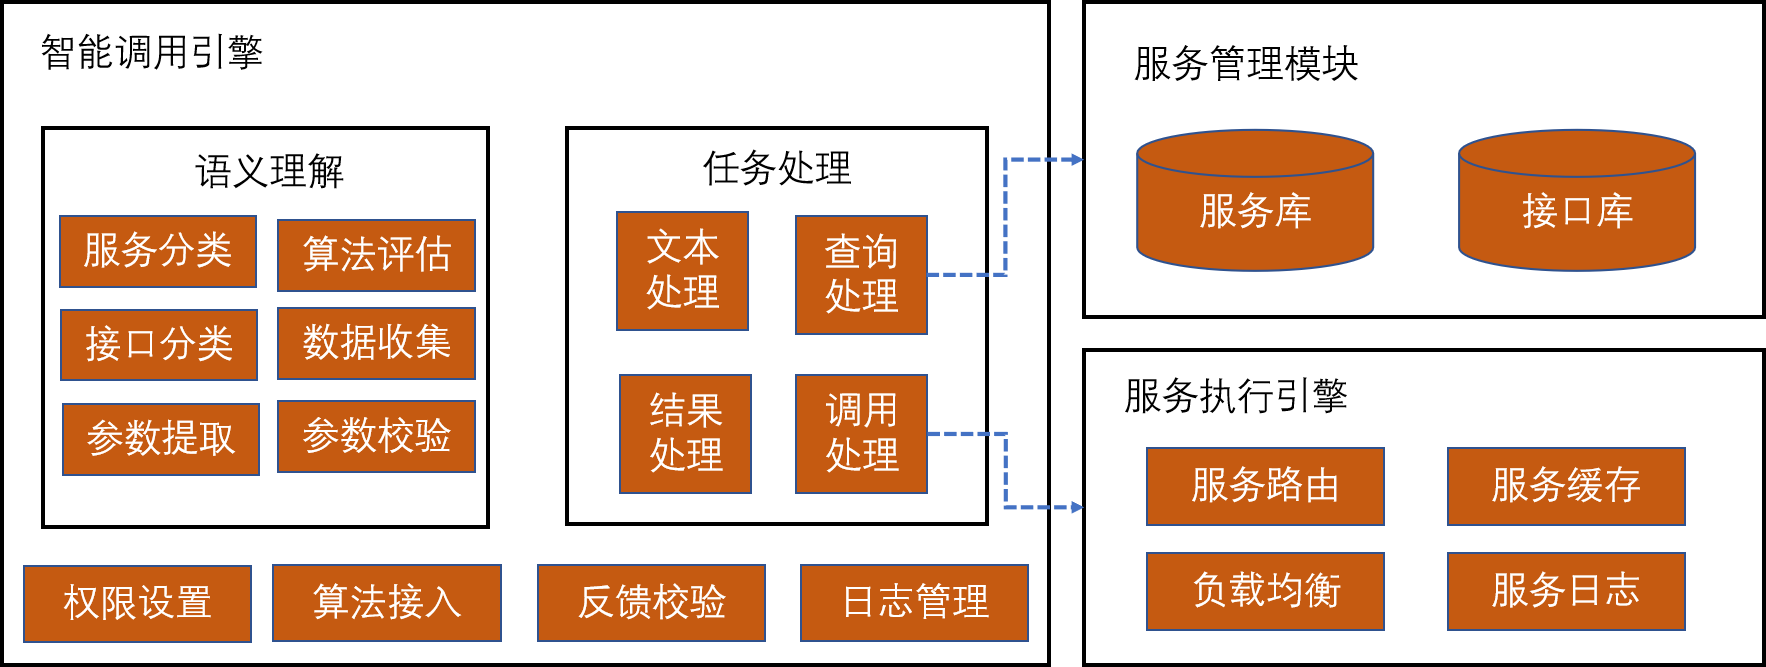
\includegraphics[width=15cm]{./images/yinqing.png}
  \caption{服务智能调用引擎架构}
  \label{fig:yinqing}
\end{figure}

如图\ref{fig:yinqing}所示,智能服务调用引擎可以抽象为语义理解和任务调度两个模块:

(1)语义理解:核心任务是本文一直在讨论的三项任务服务分类、接口分类和参数填充,接收的是用户输入的一句有目的性的话,识别用户的意图,根据
用户意图匹配相应的服务以及匹配该服务要执行的操作,找到匹配的服务以后,从用户输入的语句中提取在服务执行前需要
的执行参数,该模块算法采用的是实验性能最优的BERT-co-interactive模型。此外我们增加了数据收集模块,在每次调用之后,引擎会自动收集本次输入的语句作为数据保存,
以此来丰富平台的数据集,同时我们计划定期人工评估算法准确率进而优化模型。

(2)任务调度:该模块主要是智能调用需要解决的工程问题,使引擎能与跨界服务网络系统结合。文本处理器主要做了边界字符和停用词过滤处理,处理好的语句传入模型输入层,模型识别
出本次服务调用需要的服务、接口和参数信息后,会首先通过查询处理器向系统中服务管理模块按关键字查询得到被调用服务在系统中的执行逻辑,这里会有一个校验逻辑,校验
内容包括调用者的权限合法性以及参数信息是否有误等,校验通过以后,调用处理器会带着必要的各项参数向服务执行引擎发送请求,在跨界服务网络中找到服务源完成本次
服务的调用并返回结果到结果处理器,经结果处理器封装的最终结果会返回给用户。

如图\ref{fig:yinqingliucheng}所示,描述了智能服务调用引擎运行流程,流程大致可分为三个部分:

第一部分是交互模块。交互模块主要将用户传来的语句进行预处理传入智能解析模块,同时将系统执行服务调用
后的结果进行封装返回给前台调用者。

第二部分是智能解析模块。这其中主要逻辑就是本文重点研究的语义理解算法,包括服务分类、接口分类和参数提取,同时
也包含了必要的服务调用权限校验、参数校验和对话管理等逻辑。

第三部分是服务执行模块。该模块根据解析用户意图以后得到的信息在跨界服务网络中查询到相应服务的位置,完成服务调用后
返回执行结果到输入输出模块。

\subsection{交互模块}
交互模块是与前台距离最近的一层,因此需要在后端暴露相应的接口供前端调用。在课题组已有的JTangYdrail系统中,后端采用java语言springboot框架实现,因此
交互模块使用相同的方式,至于用户实际使用的前台产品,可以是网页或者客户端,这与跨界服务网络本身解耦。

以http请求为例,用户在前端输入带有意图的语句通过http传入交互模块的后台接口,解析出数据以后得到用户语句,
首先会进行用户权限的校验以及安全信息(如token等)的校验以验明用户身份和权限。
然后会进入输入处理模块进行文本预处理。
文本的预处理特别重要,如果句子中包含了太多无关词(这些词被称作停用词),算法性能会受影响,因此本文
在文本预处理时引用了停用词过滤。比较常见的中文停用词如“的”、“在”以及语气词等,他们的存在对语义理解没有贡献,相反如果分词工具使用他们错误的分词,
会降低模型准确率,本文利用网上已有的中文停用词词典在结巴分词工具处理前对用户语句做了停用词过滤。处理好之后的用户语句被传入智能解析模块进行语义理解分析。

在后台系统完成服务智能调用以后,交互模块会对本次服务调用进行postprocess,包括异常处理和数据封装等。异常的产生是由于跨界服务网络环境在不断动态变化,
上传在服务交换机的服务可能由于内部原因变得无法使用,同时节点信息在网络中更新有延迟,因此引擎可能检索出已不存在的服务从而产生服务调用异常,除此之外,
网路中服务路由器连接不可达导致服务调用请求无法被接受等原因也可能导致异常。如若服务成功调用并返回,由于服务种类众多返回结果的数据类型也是形态各异,
因此需要交互模块做统一的数据封装对外返回httpResponse结果。

\subsection{智能解析}
智能解析是智能服务调用引擎的核心,解决的是任务型对话系统的核心诉求,即识别用户的意图,根据
用户意图匹配相应的服务以及匹配该服务要执行的操作,找到匹配的服务以后,从用户输入的语句中提取在服务执行前需要
的执行参数,此模块由以下几个小模块组成:

(1)服务库、接口库。

(2)语义理解。 

(3)对话状态。

(4)响应逻辑。

\subsection{服务调用}


\section{原型系统展示}
在跨界服务理论基础上,实现了跨界服务网络平台的原型系统,系统被命名为JTangYdrail(图\ref{fig:logo})。
跨界服务网络与支撑载体系统依托于课题《跨界服务集成方法与支撑载体》,包含跨界服务交换机子系统、跨界服务路由器子系统和
跨界服务网络子系统。通过跨界服务交换机子系统,可以实现企业服务的包装、开放、部署和管理,并提供相关原生工具;通过跨界服务路由器
子系统,可以实现服务路由器的管理与可视化监控,实时掌握当前路由器的运行情况;通过跨界网络子系统,可以实现对全局
所有自网络及其关联的服务交换机和服务路由器的动态监控,并可对子网络进行管理。

\begin{figure}[htbp]
  \subfloat[JTangYdrail 首页]{
    \centering
    
\includegraphics[width=8cm]{./images/ketisan.png}
    \label{fig:ketisan}
  }
  \subfloat[JTangYdrail logo]{
    \centering
  
\includegraphics[width=8cm]{./images/jianmu.jpg}
  \label{fig:logo}
  }
  \caption{JTangYdrail总览}
  \end{figure}
  如图所示,JTangYdrail系统主要包含服务交换机管理、服务交换机工具和服务智能调用三个模块\ref{fig:sangemokuai}。
  服务交换机管理模块是系统的核心部分,主要包括服务管理,流程管理,申请管理和用户管理等功能,管理跨界服务网络中与服务相关
  的所有信息;服务交换机工具工具模块包括标注服务映射,物联网服务,服务包装等功能,这些功能均以工具形式嵌入JTangYdrail系统,
  是系统的附加能力;服务智能调用是与本文相关的模块,在跨界服务网络中暴露智能调用的能力,对用户输入的语句识别后智能执行相应的服务。

  \begin{figure}[htbp]
    \centering
    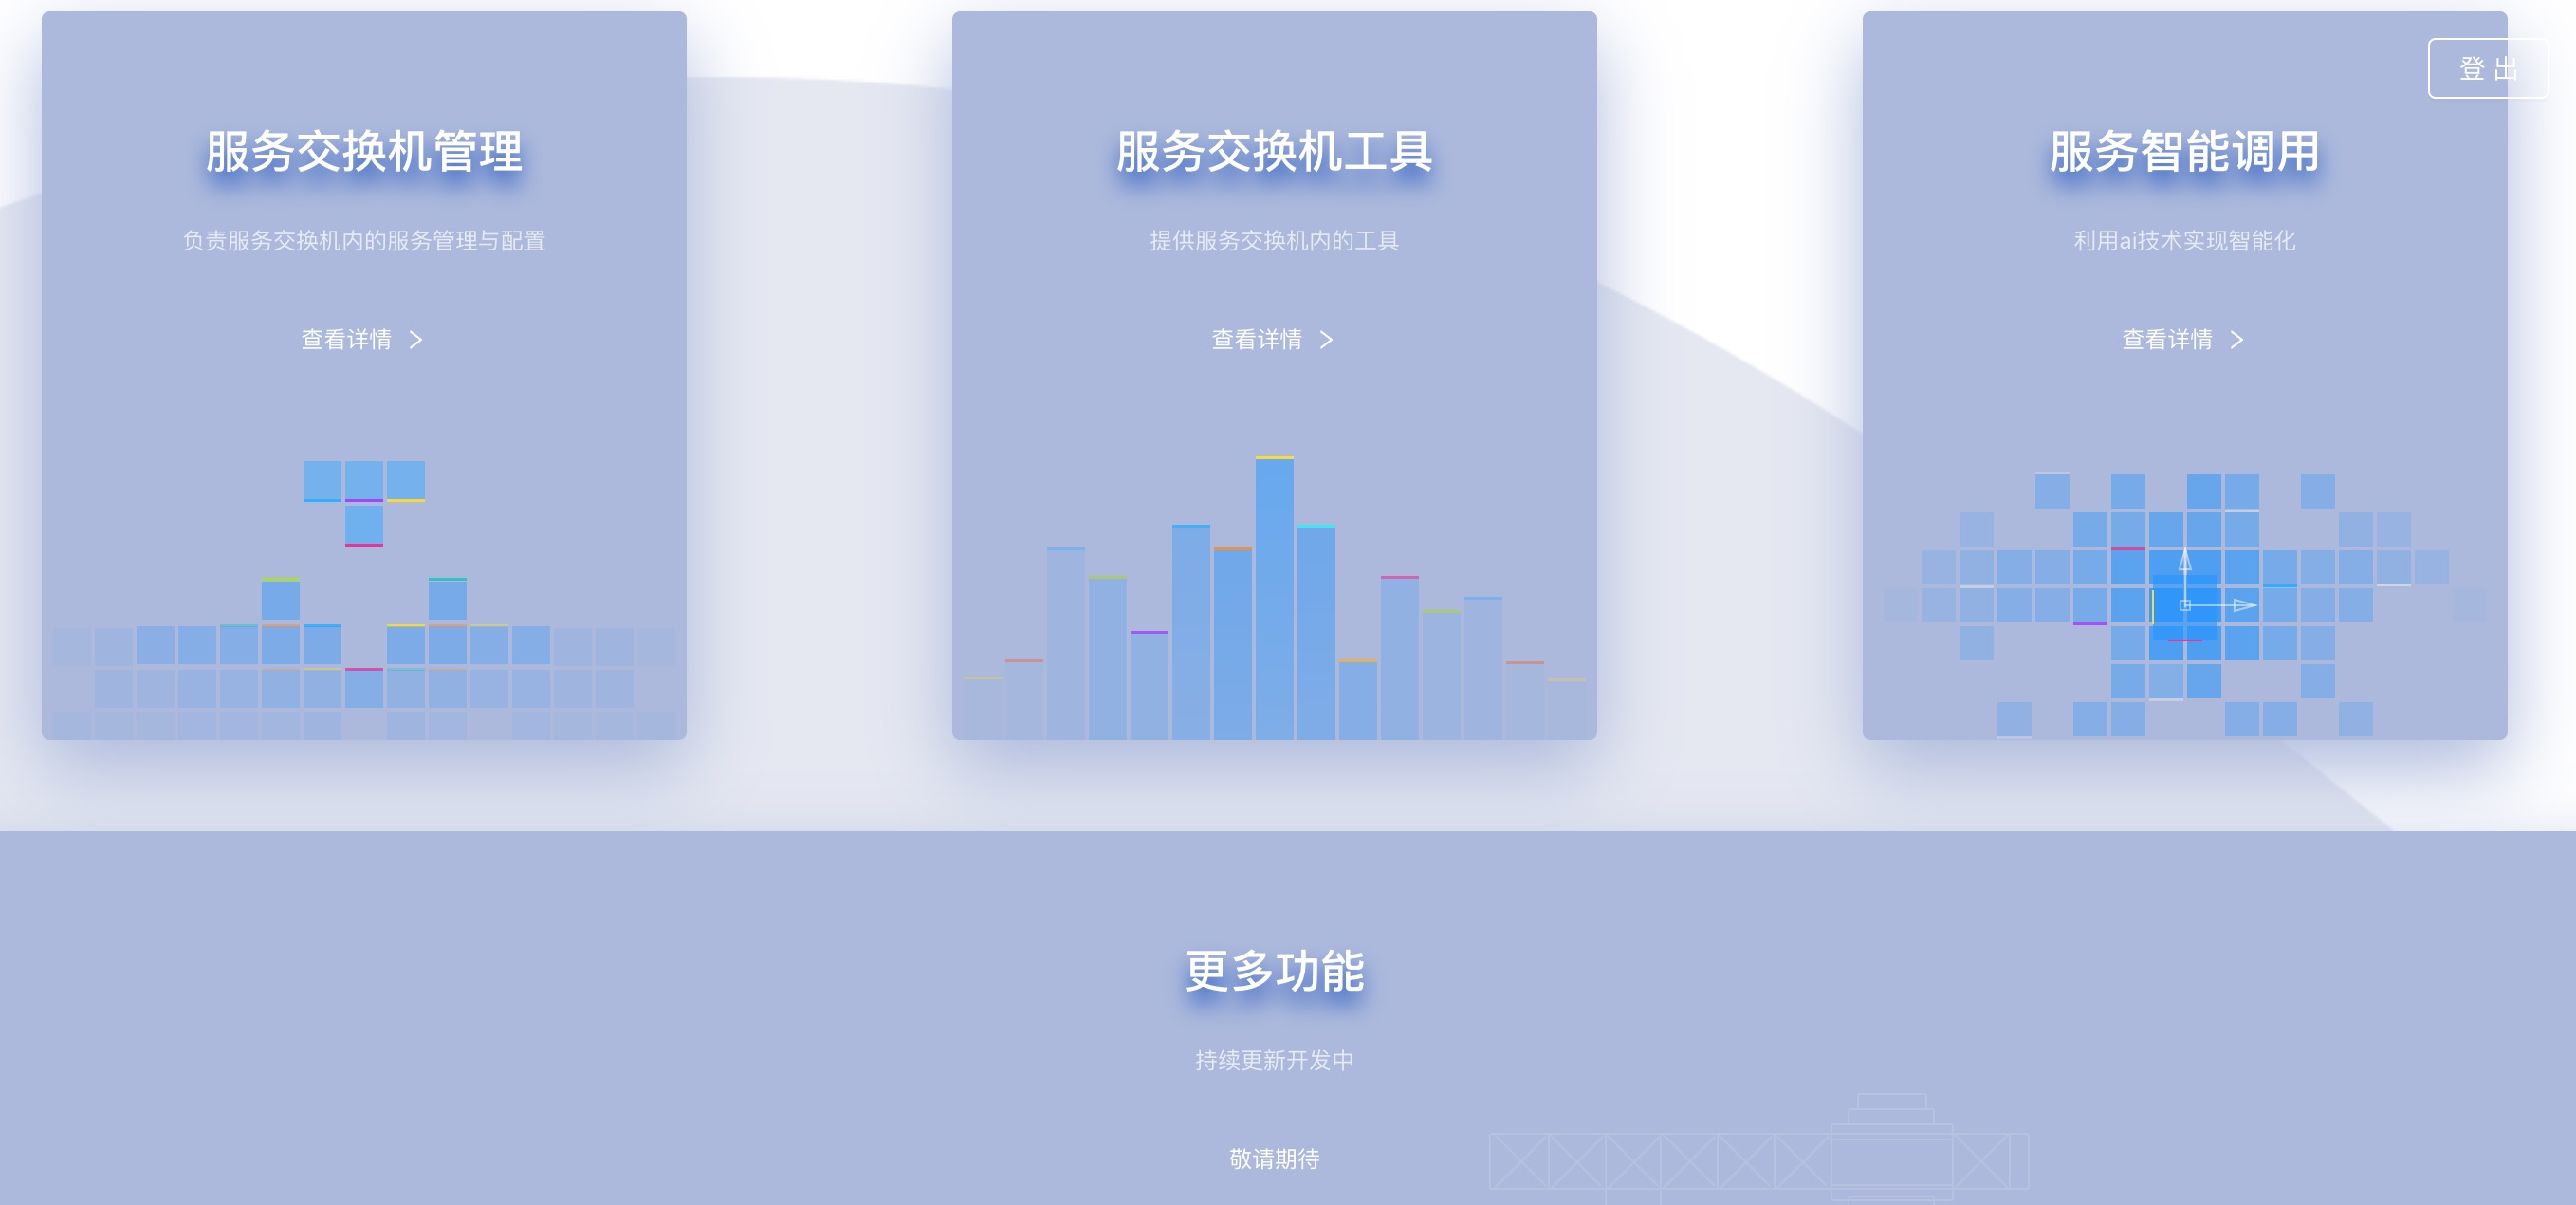
\includegraphics[width=17cm]{./images/sangemokuai.png}
    \caption{JTangYdrail 主要模块}
    \label{fig:sangemokuai}
  \end{figure}

本模块是系统的核心部分,进入系统后,点击服务详情页面对服务做CRUD,mapping,api management,test等一系列相关管理操作,
以及查看服务API的interface信息,parameter信息和SDK信息等。

如图\ref{fig:fuwuguanli}为服务管理模块的展示,服务管理的主要功能为: 
总览当前交换机内部所有服务的信息和实现对服务的增删改以及设置服务启用状态,
流程管理的主要功能为总览当前交换机内部所有流程的信息和实现对流程的增删改以及设置流程状态,
服务申请管理主要包含
企业对外进行服务申请需要的界面,可以申请其他服务交换机上的服务并实时反馈对方的审核信息,
部门管理的主要功能为
管理服务交换机中的各个部门,包括对部门信息的增删改查以及查看挂载在部门下的服务,
外部服务审批管理的主要功能为审核外部服务申请。
\begin{figure}[htbp]
  \subfloat[服务管理]{
    \centering
    \includegraphics[width=8.3cm]{./images/fuwuguanli1.png}
    \label{fig:fuwuguanli1}
  }
  \subfloat[服务详情]{
    \centering
  \includegraphics[width=8cm]{./images/fuwuguanli2.png}
  \label{fig:fuwuguanli2}
  }
  \caption{服务交换机管理模块}
  \label{fig:fuwuguanli}
  \end{figure}

%   \subsection{服务交换机工具模块}
%   本模块包括标准服务映射,物联网服务,服务包装等功能,其中标准服务映射是核心。
%   标准服务映射围绕在研究跨界服务集
%   成和交互过程中发现的 Web API 描述文档缺乏、描述方式不一致等导致的集成困难、难以
%   交互,以及服务使用者使用 Web API 过程中遇到的门槛较高、难以上手,需要根据自身需
%   求进行包装和定制操作,同类服务难以选择,以及 Web API 演化导致的应用失败等实际问
%   题进行了深入的研究和分析,提出了一套以服务映射为基础的自定义服务的解决方案,不但能够有效解决跨系统的 Web API 集成问题,而且提出了以用
%   户为中心的 Web API 的使用方式,能够大大简化和改善用户使用 Web API 的流程和体验,
% 还能够避免 Web API 演化带来的应用失败的问题。
%   \begin{figure}[htbp]
%     \subfloat[标准服务映射]{
%       \centering
%       \includegraphics[width=8cm]{./images/fuwugongju1.png}
%       \label{fig:fuwugongju1}
%     }
%     \subfloat[物联网服务]{
%       \centering
%     \includegraphics[width=8cm]{./images/fuwugongju2.png}
%     \label{fig:fuwugongju2}
%     }
%     \caption{服务交换机工具模块}
%     \label{fig:fuwugongju}
%     \end{figure}
\section{本章小结}
本章首先介绍了跨界服务网络的系统架构以及其核心组件服务交换机和服务路由器,之后介绍了智能服务调用引擎的系统架构,
最后展示了课题组目前跨界服务网络平台的原型系统JTangYdrail。


% \chapter{假的}

\section{课题背景}

九齿钉耙学名{\kaishu 上宝沁晶耙},是俺的武器。九齿钉耙并非普通的农具,而是由太上老君\footnote{太上老君,三清之第三位。又称“道德天尊”、“混元老君”、“降生天尊”、“太清大帝”等。}用神冰铁亲自锤炼,借五方五帝、六丁六甲之力锻造而成,有诗为证:

7777

% \begin{tabbing}
% \hspace{20mm} \= \hspace{20mm} \= \hspace{80mm} \kill\\
%  \> 字体      \>  \hspace{26mm} 示例 \\
%  \> fangsong \> \fangsong 老君自己动钤锤,荧惑亲身添炭屑。 \\
%  \>          \> \fangsong 五方五帝用心机,六丁六甲费周折。 \\
%  \>          \> \fangsong 造成九齿玉垂牙,铸就双环金坠叶。 \\
%  \> heiti    \> \heiti 身妆六曜排五星,体按四时依八节。 \\
%  \>          \> \heiti 短长上下定乾坤,左右阴阳分日月。 \\
%  \>          \> \heiti 六爻神将按天条,八卦星辰依斗列。 \\
%  \> kaishu    \> \kaishu 名为上宝沁金钯,进与玉皇镇丹阙。 \\
%  \>          \> \kaishu 因我修成大罗仙,为吾养就长生客。 \\
%  \>          \> \kaishu 敕封元帅号天蓬,钦赐钉钯为御节。 \\
%  \> lishu    \> \kaishu 举起烈焰并毫光,落下猛风飘瑞雪。 \\
%  \>          \> \kaishu 天曹神将尽皆惊,地府阎罗心胆怯。 \\
%  \>          \> \kaishu 人间那有这般兵,世上更无此等铁。 \\
%  \> songti   \> \songti 随身变化可心怀,任意翻腾依口诀。 \\
%  \>          \> \songti 相携数载未曾离,伴我几年无日别。 \\
%  \>          \> \songti 日食三餐并不丢,夜眠一宿浑无撇。 \\
%  \> youyan    \> \kaishu 也曾佩去赴蟠桃,也曾带他朝帝阙。 \\
%  \>          \> \kaishu 皆因仗酒却行凶,只为倚强便撒泼。 \\
%  \>          \> \kaishu 上天贬我降凡尘,下世尽我作罪孽。 \\
%  \> default  \> 石洞心邪曾吃人,高庄情喜婚姻结。 \\
%  \>          \> 这钯下海掀翻龙鼍窝,上山抓碎虎狼穴。 \\
%  \>          \> 诸般兵刃且休题,惟有吾当钯最切。 \\
%  \>          \> 相持取胜有何难,赌斗求功不用说。 \\
%  \>          \> 何怕你铜头铁脑一身钢,钯到魂消神气泄!
% \end{tabbing}

\section{各种示例}

没有规定英文字体,将中、英文统一设置为仿宋。

当存在连续多个表格、图片时,\LaTeX 的排版效果不佳,所以这里不时插播些王勃的《腾王阁序》,有空的话也看两眼。

《腾王阁序》第一段:豫章故郡,洪都新府。星分翼轸,地接衡庐。襟三江而带五湖,控蛮荆而引瓯越。物华天宝,龙光射牛斗之墟;人杰地灵,徐孺下陈蕃之榻。雄州雾列,俊采星驰。台隍枕夷夏之交,宾主尽东南之美。都督阎公之雅望,棨戟遥临;宇文新州之懿范,襜帷暂驻。十旬休假,胜友如云;千里逢迎,高朋满座。腾蛟起凤,孟学士之词宗;紫电青霜,王将军之武库。家君作宰,路出名区,童子何知,躬逢胜饯。

《腾王阁序》第二段:时维九月,序属三秋。潦水尽而寒潭清,烟光凝而暮山紫。俨骖騑于上路,访风景于崇阿。临帝子之长洲,得天人之旧馆。层台耸翠,上出重霄;飞阁翔丹,下临无地。鹤汀凫渚,穷岛屿之萦回;桂殿兰宫,即冈峦之体势。披绣闼,俯雕甍:山原旷其盈视,川泽纡其骇瞩。闾阎扑地,钟鸣鼎食之家;舸舰迷津,青雀黄龙之轴。云销雨霁,彩彻区明。落霞与孤鹜齐飞,秋水共长天一色。渔舟唱晚,响穷彭蠡之滨;雁阵惊寒,声断衡阳之浦。

\subsection{图片示例}

附上照片一张,来源 Wikipedia。

\begin{figure}[htbp]
  \centering
  \includegraphics[scale=0.5]{./images/zhubajie.png}
  \caption{玉照,玉做的照片,通常会令人联想到浴照。}
  \label{fig:example}
\end{figure}

我来插两张并排的图像,其实\LaTeX 支持jpg, png, 以及eps格式的图片,图\ref{fig:tangseng}是我的师傅,帅吧!

\begin{figure}[htbp]
\centering
\subfloat[师傅]{
\includegraphics[width=6cm]{./images/tangseng.jpg}
\label{fig:tangseng}
}
\hspace{60pt}
\subfloat[大师兄]{
\includegraphics[width=6cm]{./images/sunwukong.png}
\label{fig:sunwukong}
}
\caption{你挑着担,我写代码...}
\end{figure}

\subsection{表格示例}

\LaTeX 中的表格不是很好搞,看起来很不直观,不过我们一般不会用太高端的表格,更多关于表格的请看\texttt{Helin Gai}的\textsf{\LaTeX Manual}\cite{gaiart}以及
\texttt{Alpha Huang}的\textsf{lnotes}\cite{lnotes}

先看一个简单表格 \ref{tab:simple-table}:

\begin{table}[htb]
  \centering
  \caption{模板中的表格宏包}
  \label{tab:simple-table}
    \begin{tabular}{ll}
      \toprule
      \multicolumn{1}{m{20mm}}{\heiti\centering 宏包} & \multicolumn{1}{m{80mm}}{\heiti\centering 描述} \\
      \midrule
      longtable & 绘制跨页的表格。 \\
      booktabs & 三线表中的那三条线的命令来自这里。\\
      caption2 & 用于设置标题很方便,已经 obsolated,不过 \TeX Live 中还有。\\
      multirow & 跨行的单元格用这个宏包。\\
      dcolumn  & 想让表格小数点对齐吗?用这个宏包吧。\\
      \rowcolor[gray]{.9} colortbl & 表格上色。自己看着爽而已,打印出来都是黑白的。 \\
      threeparttable & 用来给表格添加脚注啥的很方便。 \\
      array & 忘了用来做什么了,但似乎很重要。 \\
      \bottomrule
    \end{tabular}
\end{table}


\subsection{公式示例}

我公式用非常少,所以公式的情况并不了解,这部分示例也完全照搬 。如果有什么问题或要求,可以贴到 88 \TeX 版。

贝叶斯公式如式 (\ref{equ:chap1:bayes}),其中 $p(y|\mathbf{x})$ 为后验;$p(\mathbf{x})$ 为先验;分母 $p(\mathbf{x})$ 为归一化因子。

\begin{equation}
\label{equ:chap1:bayes}
p(y|\mathbf{x}) = \frac{p(\mathbf{x},y)}{p(\mathbf{x})}=
\frac{p(\mathbf{x}|y)p(y)}{p(\mathbf{x})} 
\end{equation}

论文里面公式越多,\TeX 就越 happy。再看一个 \textsf{amsmath} 的例子:

\newcommand{\envert}[1]{\left\lvert#1\right\rvert} 

\begin{equation}\label{detK2}
\det\mathbf{K}(t=1,t_1,\dots,t_n)=\sum_{I\in\mathbf{n}}(-1)^{\envert{I}}
\prod_{i\in I}t_i\prod_{j\in I}(D_j+\lambda_jt_j)\det\mathbf{A}
^{(\lambda)}(\overline{I}|\overline{I})=0.
\end{equation} 

大家在写公式的时候一定要好好看 \textsf{amsmath} 的文档,并参考模板中的用法:

\begin{multline*}\tag{[b]} % 这个出现在索引中的
\int_a^b\biggl\{\int_a^b[f(x)^2g(y)^2+f(y)^2g(x)^2]
 -2f(x)g(x)f(y)g(y)\,dx\biggr\}\,dy \\
 =\int_a^b\biggl\{g(y)^2\int_a^bf^2+f(y)^2
  \int_a^b g^2-2f(y)g(y)\int_a^b fg\biggr\}\,dy
\end{multline*}

其实还可以看看这个多级规划:

\begin{equation}\label{bilevel}
\left\{\begin{array}{l}
\max\limits_{{\mbox{\footnotesize\boldmath $x$}}} F(x,y_1^*,y_2^*,\cdots,y_m^*)\\[0.2cm]
\mbox{subject to:}\\[0.1cm]
\qquad G(x)\le 0\\[0.1cm]
\qquad(y_1^*,y_2^*,\cdots,y_m^*)\mbox{ solves problems }(i=1,2,\cdots,m)\\[0.1cm]
\qquad\left\{\begin{array}{l}
    \max\limits_{{\mbox{\footnotesize\boldmath $y_i$}}}f_i(x,y_1,y_2,\cdots,y_m)\\[0.2cm]
    \mbox{subject to:}\\[0.1cm]
    \qquad g_i(x,y_1,y_2,\cdots,y_m)\le 0.
    \end{array}\right.
\end{array}\right.
\end{equation}

\subsection{定理示例}

THUThesis定义了很多定理格式,THUThesis下面都是从来的例子。我自己只用到了“假设”,对于公式、证明之类的格式完全无知,你如有其他需要可以在 88 \TeX 版上提出来,我再添加。

\begin{hypo}
  
\begin{eqnarray}
  \label{eq:eqnxmp}
  c & = & a^2 - b^2\\
    & = & (a+b)(a-b)
\end{eqnarray}
\end{hypo}

\begin{defin}
子曰:「道千乘之国,敬事而信,节用而爱人,使民以时。」
\end{defin}

\begin{theo}
犯我强汉者,虽远必诛。\hfill —— 陈汤(汉)
\end{theo}

\begin{pro}
天不言自高,水不言自流。
\begin{gather*}
\begin{split} 
\varphi(x,z)
&=z-\gamma_{10}x-\gamma_{mn}x^mz^n\\
&=z-Mr^{-1}x-Mr^{-(m+n)}x^mz^n
\end{split}\\[6pt]
\begin{align} \zeta^0&=(\xi^0)^2,\\
\zeta^1 &=\xi^0\xi^1,\\
\zeta^2 &=(\xi^1)^2,
\end{align}
\end{gather*}
\end{pro}

\subsection{算法示例}

大家有时候还需要写一些算法的伪代码,不用蛋疼,模板里面已经有支持了,看看算法\ref{alg:put-into-refri},具体的实用还需要参考CTAN上的关于{\textsf{algorithmicx}}宏包的文档,包括自定义关键字等等。

\begin{algorithm}
\caption{把猪八戒放进冰箱}
\label{alg:put-into-refri}
\begin{algorithmic}[1]
\Require N头动物,不知道是不是猪八戒  \Comment{我是注释} 
\Ensure 你造吗,这个程序木有输出,想怎样?
\State 先热热身:)
\For{$i=1,\dots ,N$} \Comment{我是个For循环}
\If {是猪八戒}
	\State 打开冰箱门,把第$i$个放进冰箱,关上冰箱门
\Else 
	\State 下一个
\EndIf
\EndFor
\end{algorithmic}
\end{algorithm}

\subsection{参考文献}

参考文献建议使用 BiB\TeX 。

参考文献的例子:书籍文献\cite{tex,companion};杂志文章,单独的\cite{article1},并列的\cite{article2,article3},合并的\cite{article1,article2,article3};硕士论文\cite{master},俺的旧文一篇;博士论文\cite{doctor},沙师弟的大作;论文集或 Handbook\cite{collection},会议论文集\cite{proceeding},会议论文\cite{conference};带页码脚标的\cite[123]{tex}。




% \chapter{假的}

这是第二章,目的是占个位置。你知道《浙大同学爱占坐》这首歌吗?


\ZJUbackmatter
%%%%%%%%%%%%%%%%%%%%%%%%%%%%%%
%% 参考文献
%%%%%%%%%%%%%%%%%%%%%%%%%%%%%%
\ZJUthesisbib{thesisbib}

%%%%%%%%%%%%%%%%%%%%%%%%%%%%%%
%% 发表论文目录
%%%%%%%%%%%%%%%%%%%%%%%%%%%%%%
\begin{publications}

% \textbf{已发表论文}
% \begin{itemize}


% \end{itemize}



\noindent \textbf{\large {1.已发表论文}}

Meng Xi, Jianwei Yin, Yongna Wei, Maolin Zhang, et al. A Scenario-based Modeling Method for Crossover Services.
IEEE International Conference on Services Computing (SCC),2020.
$\\$

\noindent \textbf{\large 2.发明专利}

一种基于交互式联合识别模型的跨界服务平台内服务智能调用的方法(提交中)
$\\$

\noindent \textbf{\large 3.主要参与项目}

跨界服务融合理论与关键技术,国家重点研发计划,课题编号:SQ2017YFB140121-03


\end{publications}


%%%%%%%%%%%%%%%%%%%%%%%%%%%%%%
%% 致谢页
%%%%%%%%%%%%%%%%%%%%%%%%%%%%%%
\begin{thanks}
感谢导师唐三藏的温柔和慈爱,不计时间给予俺无微不至地教诲,让俺在如雨般的唾沫星下滋润成长。

感谢师兄孙悟空的肢体教育,让俺成功减肥,俺和俺身上的每一块青紫都会记住你的。

感谢师弟沙悟净的任劳任怨,得失无争。

感谢高小姐的一片真情,可叹俺已遁入空门、修成正果。当年你在情人坡娇怨俺没貌没地位,现在俺终于位列仙班,可却注定要永远分离,缘何俺们总是“错位”……

\begin{flushright}
{\kaishu{
  \large{猪悟能}\hspace{0.5in}

  \large{2013年1月于大雷音寺}\hspace{0.18in}
}}

\end{flushright}

\end{thanks}



\end{document}
